\documentclass[a4paper,11pt]{book}

%\usepackage[breakable]{tcolorbox}
\usepackage{parskip} 
   \providecommand{\tightlist}{\setlength{\itemsep}{0pt}
                               \setlength{\parskip}{0pt}}                              
\usepackage{geometry} % Used to adjust the document margins
    \geometry{verbose,tmargin=1in,bmargin=1in,lmargin=1in,rmargin=1in}
\usepackage{amsmath} % Equations
\usepackage{amssymb} % Equations
\usepackage{titling} % Toglie spazi esagerati ai titoli
\usepackage{graphicx}  % Per immagini
\usepackage[Export]{adjustbox} % Constrain images to a maximum size
    \adjustboxset{max size={0.9\linewidth}{0.9\paperheight}}
\usepackage{float}
    \floatplacement{figure}{H}
\usepackage{xcolor}
  \definecolor{mygreen}{rgb}{0,0.6,0}
  \definecolor{mygray}{rgb}{0.95,0.95,0.95}
  \definecolor{mymauve}{rgb}{0.58,0,0.82}  
  \definecolor{urlcolor}{rgb}{0,.145,.698}
  \definecolor{linkcolor}{rgb}{.71,0.21,0.01}
  \definecolor{citecolor}{rgb}{.12,.54,.11}
\usepackage{hyperref}
    \hypersetup{
      breaklinks=true,  % so long urls are correctly broken across lines
      colorlinks=true,
      urlcolor=urlcolor,
      linkcolor=urlcolor,
      citecolor=citecolor,
      }    
\usepackage{listings} % per il codice

\lstset{ 
  backgroundcolor=\color{mygray},  
  basicstyle=\footnotesize,       
  breakatwhitespace=false,        
  breaklines=true,                
  captionpos=b,                   
  commentstyle=\color{mygreen},   
  escapeinside={\%*}{*)},        
  extendedchars=true,            
  firstnumber=1,               
  frame=single,	
  language=java,                  
  keepspaces=true,                
  basicstyle=\footnotesize\ttfamily,           
  numbers=left,                  
  numbersep=5pt,                 
  numberstyle=\tiny\color{black}, 
  rulecolor=\color{black},                        
  stepnumber=1,                        
  tabsize=2,	                      
}
   
% ===============================================================
\graphicspath{
              {../1_premises/img/},
              {../2_instruments/img/},
              {../3_fixed/img/},
              {../4_cmusic/img/}
              }

\begin{document}

\author{Andrea Vigani}
\title{Electroacoustic composition}
\maketitle

%\begin{abstract}
%In this Chapter bla bla bla.
%\end{abstract}

\tableofcontents

\chapter{Premises}

\section{Preliminary reflections}\label{preliminary-reflections}

Music composition

What does it mean?

To compose, to assemble, to put together something.

Let's tackle some basic concepts about in no particular order.

\subsection{Concrete things}\label{concrete-things}

Before producing any sound we must choose or assemble a physical object.

\begin{center}
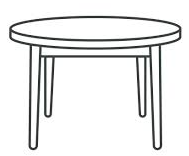
\includegraphics[scale=0.45]{../img/tavolo.png}
\end{center}

Pyhsical object with elestic characteristics can be exited in some way producing sound waves.

\begin{center}
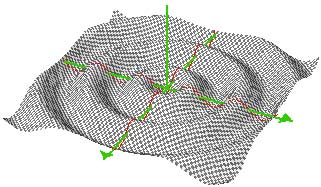
\includegraphics[scale=0.55]{../img/pelle.png}
\end{center}

Sound waves are a form of energy that propagates in time and space through an elastic medium.

Sound waves simply exist in our world.

When a sound wave reaches our ears it is perceived as an acoustic information by our brain.

\begin{center}
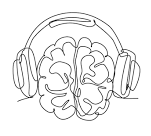
\includegraphics[scale=0.5]{../img/percezione.png}
\end{center}

It's a concrete thing.

When it was choosen or assembled:

\begin{itemize}
\tightlist
\item we can interact with it (touch it, move it, etc.).
\item we can make a copy (a model).
\item we can modify it (improve it).
\item we can destroy (or forgot) it.
\item it does not require linguistic representation, it simply be.
\item it exist in space and not necessary in time.
\end{itemize}

This has to do with the physical world.

We live immersed in sound waves.

We listen to music more or less daily but\ldots is music always sound waves?

No.

We can think and organize sounds inside our mind without producing them as sound waves.

\begin{center}

\includegraphics[scale=0.65]{../img/musicervice.png}
\end{center}

Sound waves have to do with physical world and human perception.

Music is a complex thing that has to do with both perceptual and cognitive human systems.

\subsection{Pre-linguistic}\label{pre-linguistic}

We can compose ideas or instinctive sequences of sounds.

Putting thoughts together in a pre-linguistic manner.

\begin{center}
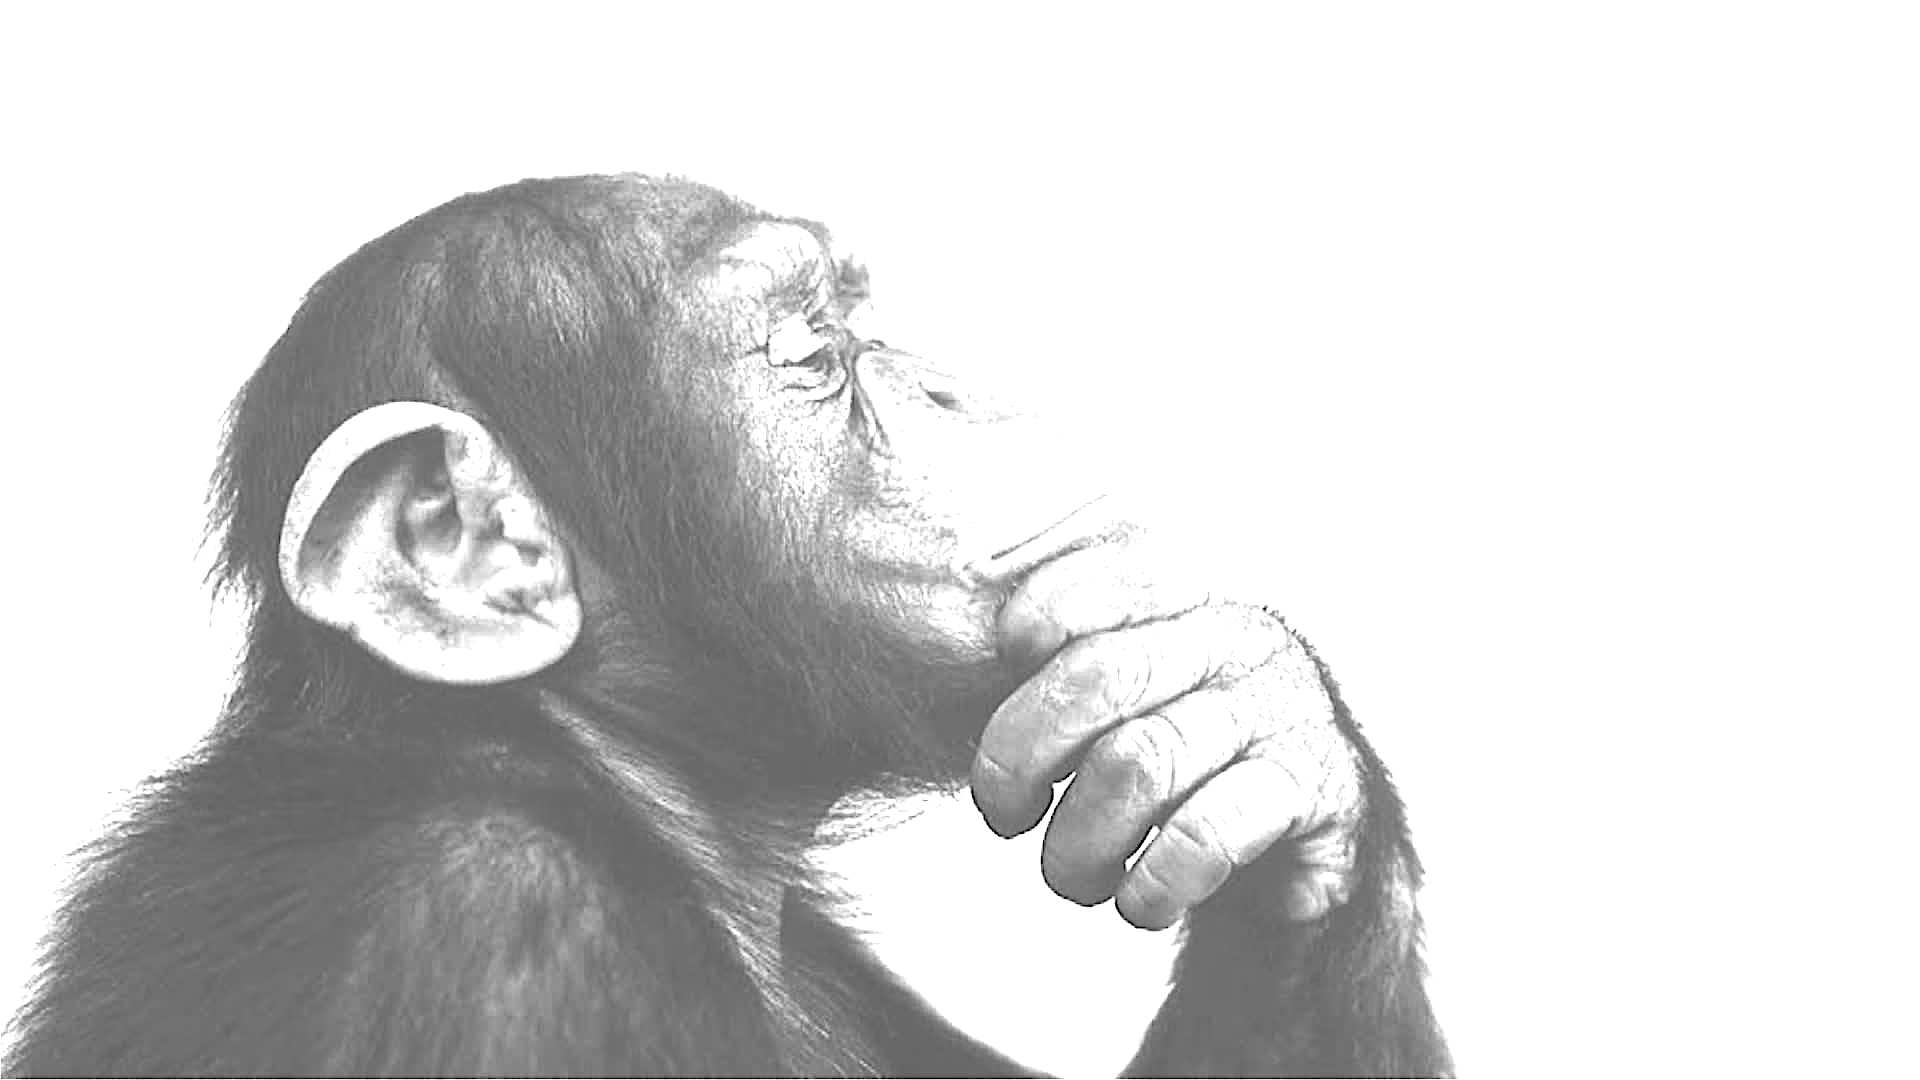
\includegraphics[scale=0.35]{../img/pensiero.png}
\end{center}

An abstract thing.

When we thinked it:

\begin{itemize}
\tightlist
\item we can't interact with it (touch it, move it, etc.).
\item we can do a copy (replicate pattern structure).
\item we can reproduce it but only in its physical forms (kinds of matter):
   \begin{itemize}
   \tightlist
   \item declaiming it (sound waves).
   \item writing it on a paper using symbolic representations.
   \end{itemize}
\item we can modify it.
\item we can't destroy it (we can only destroy its representation in physical world - book, recordings, etc. - not in our memory).
\item it does not require linguistic representation.
\item it exists in the space of consciousness (our mind) but when we
  reproduce it in the physical world it exist both in space and time.
\end{itemize}

This has to do with mind, consciousness and human expression.

Let's explore this concept through a comparison between natural language and musical language because they: 
\begin{itemize}
\tightlist
\item are universal (present in all human cultures). 
\item belong exclusively to our species. 
\item ensure the cohesion of a social group. 
\item share formal and functional characteristics.
\end{itemize}

\subsubsection{Natural language}\label{natural-language}

Psycholinguistic studies say that at a deep level all natural languages have the same structure and this can tell us something universal about the human intellect (our brain).

The form of human thought is innate and common to all members of the species.

The function of language is to express it.

\begin{center}

\includegraphics[scale=0.5]{../img/linguaggio.png}
\end{center}

The deep structure of an expression is closely related to the thought it represents.

If pre-linguistic thoughts have the same type of form for everyone the linguistic structures that represent them must also have the same type of form.

\begin{center}
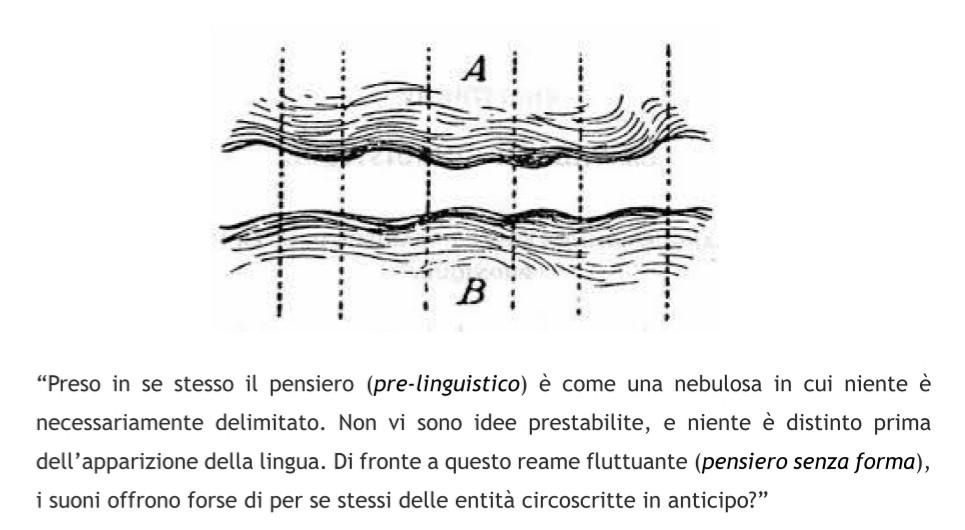
\includegraphics[scale=0.4]{../img/prelinguistico.png}
\end{center}

If we want to transform a deep thought structure into a statement we assemble it together into a linear sequence of sounds.

This sequence must convey to the listener the necessary informations for its comprehension.

Thought itself cannot be considered a linguistic sequence because it exists independently of language.

\subsubsection{Musical language}\label{musical-language}

About music there exist forms of mental activity independent of any musical language such as \href{http://www.musicaecodice.it/gitmedia/emc/1_media/bimbi.mp3}{children's nursery rhymes} or \href{http://www.musicaecodice.it/gitmedia/emc/1_media/tibet.mp3}{tibetan songs}.

Pre-linguistic musical thought must be an abstract scheme that includes exclusively the characteristics common to all musics.

If both music language and natural language are universal characteristics of the human specie this means that humans have a natural capacity to acquire both linguistic and musical skills.

Natural language and musical language expressions are conveyed in the real world in the form of sound waves.

The sound waves common basic physical parameters are: 

\begin{itemize}
\tightlist
\item frequency \(\rightarrow\) interval, pitch, intonation. 
\item amplitude \(\rightarrow\) dynamic. 
\item time \(\rightarrow\) rhythm. 
\item timbre \(\rightarrow\) instrumental techniques, vocal expressions, orchestration.
\end{itemize}

Even though surface forms differ from culture to culture we can find these universal elements not only in physical parameters but also in the subdivision into multiple levels of the languages.

\subsection{Compose a phone number}\label{compose-a-phone-number}

\begin{center}

\includegraphics[scale=0.4]{../img/telefono.png}
\end{center}

Defining a code.

\begin{itemize}
\tightlist
\item a sequence of numbers (or letters or sounds) that represents a thought.
\item we can't modify it.
\item it requires encoding and decoding.
\item to understand it we need to know its linguistic structure.
\item it follow precise and shared rules.
\item if we don't know them, the sequence of numbers or sounds makes no sense to us.
\item it require linguistic representation.
\item it can be: 
  \begin{itemize}
  \tightlist
  \item in space \(\rightarrow\) if you write it in a phone directory.
  \item in time \(\rightarrow\) if you digit it on a phone keyboard.
  \end{itemize}
\end{itemize}

This has to do with language and its representations.

Let's start again with the comparison between natural and musical language.

Leaving aside the first common level represented by the physical parameters of sound both are built on further different levels.

Simplifying, we can identify four levels:

\begin{itemize}
\tightlist
\item phonetic-phonological \(\rightarrow\) phonetics and prosody - individual notes, pitches, scales, tunings, etc.
\item morphosyntactic \(\rightarrow\) combination of phonemes into morphemes and morphemes into words - rhythm, chords, etc.
\item syntactic \(\rightarrow\) rules defining the relationships between words - counterpoint, harmony, twelve-tone system, asides, phrases, etc.
\item semantic \(\rightarrow\) access to meaning.
\end{itemize}

\subsubsection{Phonetic-phonological level }\label{phonetic-phonological-level}

It is present in all languages.

Every linguistic output can be broken down into phonemes which are a small set of sound classes.

For example the word `ape' is made up of three phonemes one for each letter.

Phonemes have two distinctive features: 

\begin{itemize}
\tightlist
\item they are not characterized by absolute values but by a set of sounds within a certain range. 
\item the continuum of sounds is divided differently in different languages (two sounds that constitute two phonemes in one language form a single phoneme in another).
\end{itemize}

\begin{center}
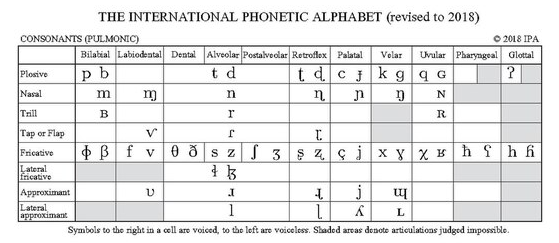
\includegraphics[scale=0.9]{../img/fonemi_2.png}
\end{center}

In western musical languages the fundamental phoneme could be considered the note with its various types of expression (staccato, tenuto, accentato, legato, etc.).

\begin{center}
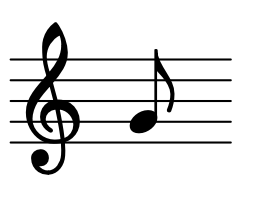
\includegraphics[scale=0.22]{../img/nota.png}
\end{center}

Let us remember that in both languages they are characterised by frequency, duration, amplitude and timbre.

\subsubsection{Morphosyntactic level }\label{morphosyntactic-level}

Phonemes can join together to form morphemes.

Morphemes can join together to form words.

Words are basic elements of language that: 

\begin{itemize}
\tightlist
\item carries meaning. 
\item can be used on its own.
\item are uninterruptible.
\end{itemize}

In music we could consider them as a short melodic pattern (inciso).

\begin{center}
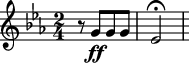
\includegraphics[scale=0.7]{../img/inci.png}
\end{center}

A vocabulary (lexicon) is a set of words in a given language.

In music we could consider it as a set of rhytmic and melodic patterns.

Substantial differences between the two languages:

\begin{itemize}
\tightlist
\item in natural language a word has a general function (the word `table' represent a table).
\item in music a specific word exist only within a piece (we can consider Beethoven's fifth symphony incise a word only in this symphony).
\end{itemize}

\subsubsection{Syntactic level }\label{syntactic-level}

Syntax or formal grammar \(\rightarrow\) a closed system of rules that serves exclusively to generate the set of sequences considered grammatical.

Every natural language like every musical language has its own syntax (Italian, French, German, counterpoint, harmony, twelve-tone, etc.).

We have previously defined that music is not necessarily conveyed through sound waves but\ldots are sound waves always music?

No, again.

In order to be defined music language requires a codification of sounds in vocabularies and systems of rules.

\begin{center}
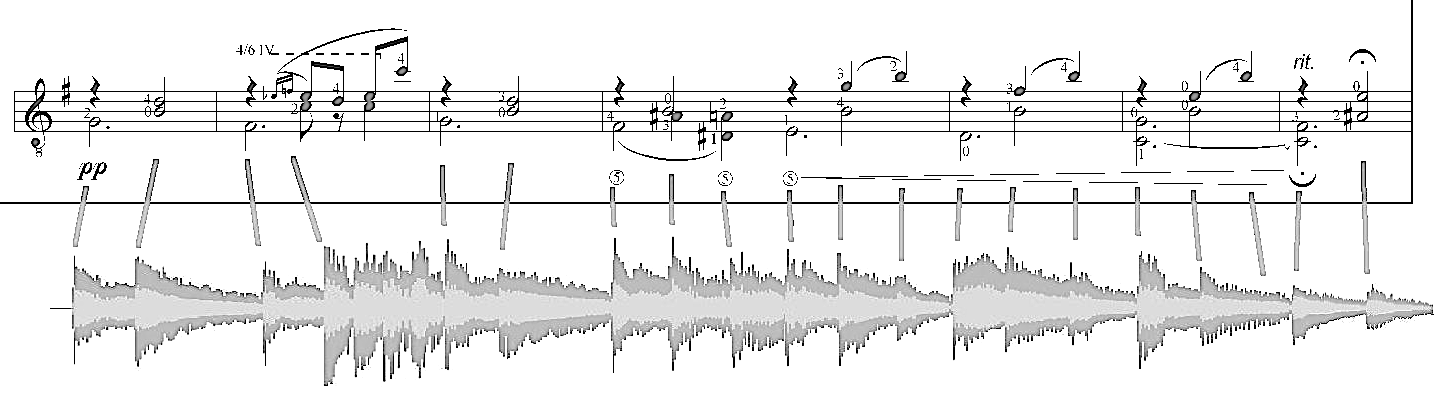
\includegraphics[scale=0.9]{../img/ondenote.png}
\end{center}

In all musical cultures the physical parameters of sound are organized in symbols.

These symbols can become independent from sound waves.

\begin{center}
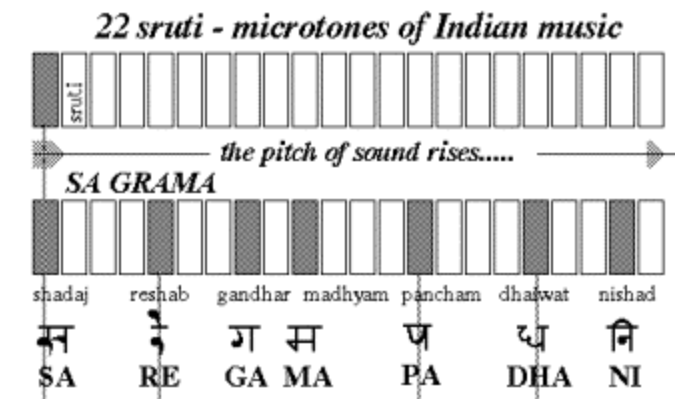
\includegraphics[scale=0.4]{../img/india.png}\break
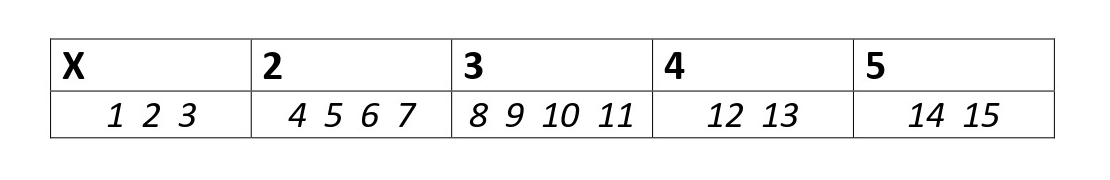
\includegraphics[scale=0.3]{../img/rtmoindia.png}
\end{center}

In Western musical tradition, from psamody until around 1940 these parameters have maintained more or less the same vocabulary over the centuries (diatonic and chromatic intervals, metric and subdivision of beat, musical instruments, etc.).

\begin{center}
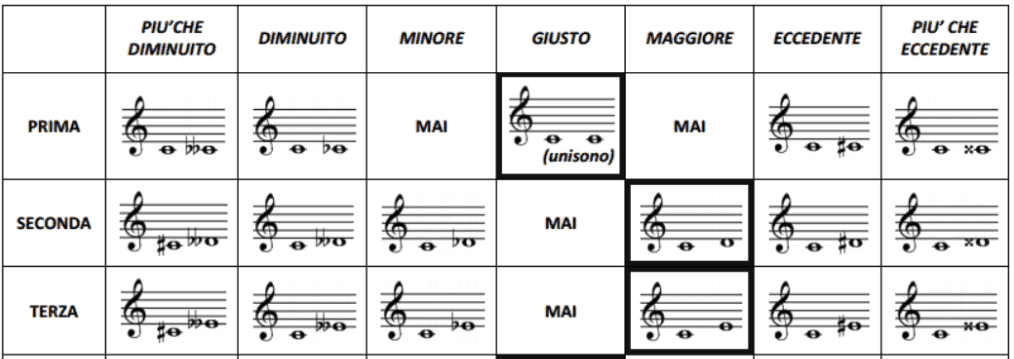
\includegraphics[scale=0.85]{../img/intervalli.png}
\end{center}

The systems of rules through which the vocabulary terms were organized (syntax), however, were different (modality, counterpoint, harmonic systems, dodecaphony, stocastic systems, alea, etc.).

\begin{center}
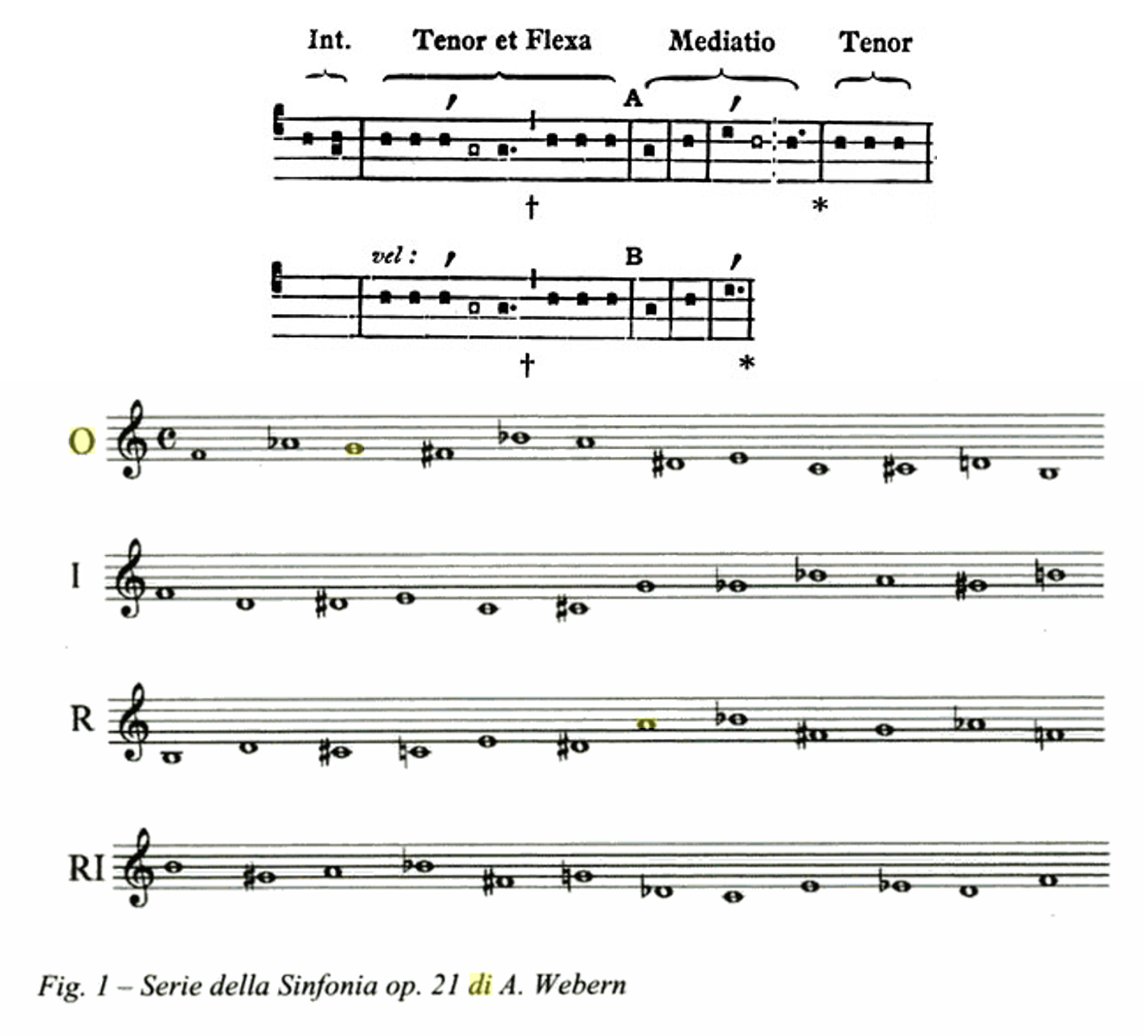
\includegraphics[scale=0.75]{../img/greg.png}
\end{center}

For this reason we cannot define western music as a single language but as a set of languages \hspace{0pt}\hspace{0pt}that use the same vocabulary (classical music, baroque music, pop music, jazz music, etc.).

Even more so if we talk about music from different cultures.

On this level the differences underlined at the end of the previous paragraph regarding musical words disappear.

Musical grammars are a meta-reflection that deals with symbolic forms.

These can be abstracted to the point of taking on a meaning of their own that goes beyond the perception of the work.

\begin{center}
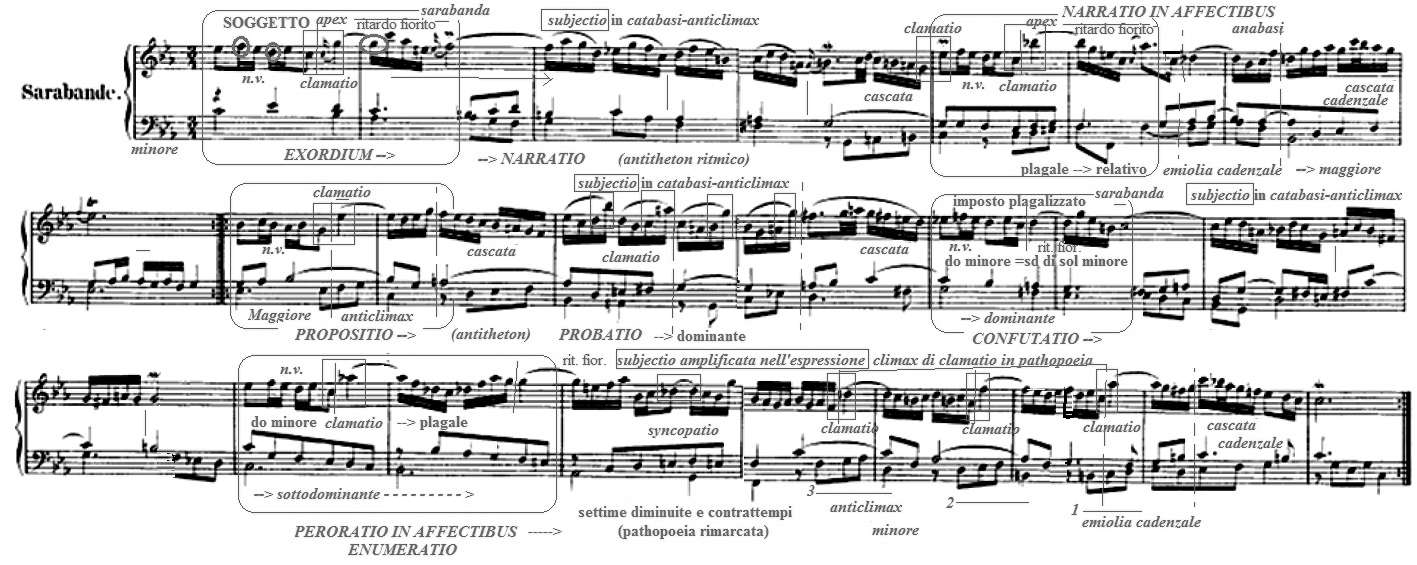
\includegraphics[scale=1.1]{../img/analisische.png}
\end{center}

\subsubsection{Semantic level}\label{semantic-level}

The branch of linguistics and logic concerned with meaning.

In musical language there are several starkly contrasting theories on this subject none of which can be assumed to be universal.

The one that summarizes the two main positions was proposed by the American musicologist L.B.Meyer who distinguishes between two forms of meaning in music:

\begin{itemize}
\tightlist
\item designative meaning \(\rightarrow\) which refers to something extramusical (G.Malher \href{http://www.musicaecodice.it/gitmedia/emc/1_media/malher.mp3}{Symphony n 10} - extract).
\item embodied meaning \(\rightarrow\) the meaning a piece has for the listener in terms of:

  \begin{itemize}
  \tightlist
  \item Internal syntactic structure.
  \item Interactions between this structure and the listener's musical knowledge and expectations. Musical structure can create expectations that can be disappointed or fulfilled generating a dynamic flow of tensions and resolutions that influence the listener's emotional and aesthetic responses. These are aesthetic emotions that have nothing to do with the emotions experienced in real life (F.Schubert \href{http://www.musicaecodice.it/gitmedia/emc/1_media/schubert.mp3}{Trio} - extract).
  \end{itemize}
\end{itemize}

Can we express in words what emotions listening to this Schubert trio arouses in us?

We will delve deeper into this last topic in the \hyperref[meaning]{Music’s meaning} section.

These levels enable common phenomena that help us understand the difference between sound waves and language.

\begin{itemize}
\tightlist
\item categorical perception \(\rightarrow\) a continuous linguistic or musical sound is segmented into discrete categorized units (phonemes, notes, words). If we repeat the same phrase or melody several times they will always be recognized as the same despite variations in acoustic parameters sometimes even significant ones (\href{http://www.musicaecodice.it/gitmedia/emc/1_media/pollini.mp3}{exemple 1}, \href{http://www.musicaecodice.it/gitmedia/emc/1_media/kissin.mp3}{exemple 2}, \href{http://www.musicaecodice.it/gitmedia/emc/1_media/sokolov.mp3}{exemple 3}).
\item phonemic restoration \(\rightarrow\) replacing part of the linguistic signal with noise simultaneously with the word or music does not affect the perception of the whole. Semantic-lexical or musical expectations prevail over acoustic analysis (\href{http://www.musicaecodice.it/gitmedia/emc/1_media/buchi.mp3}{musical},  \href{http://www.musicaecodice.it/gitmedia/emc/1_media/vian.mp3}{natural}).
\item expectations \(\rightarrow\) the syntactic construction of a sentence leads us to expect one word rather than another within it, just as happens within a sequence of chords in tonal terms (\href{http://www.musicaecodice.it/gitmedia/emc/1_media/analisi.mp3}{words}, \href{http://www.musicaecodice.it/gitmedia/emc/1_media/accordi.mp3}{chords}).
\end{itemize}

\subsection{Perceive and process }\label{perceive-and-process}

The ability to perceive and process musical information (not exclusively acoustic) is also common to all cultures.

Listening to music from one's own culture provides the listener with additional implicit information.

The simplest musical competence requires the activation of numerous cognitive abilities, including: 

\begin{itemize}
\tightlist
\item memory \(\rightarrow\) short-term recognition of melodic rhythmic patterns.
\item maintenance of attention \(\rightarrow\) active listening.
\item analysis of the temporal structure \(\rightarrow\) continuous comparison between present and short-term memory.
\end{itemize}

These abilities are part of a body of knowledge acquired through more or less conscious implicit learning that occurs through two modalities:

\begin{itemize}
\tightlist
\item universal cognitive mechanisms \(\rightarrow\) experimental psychology studies have shown that even prenatally the fetus responds to sounds and noises that activate phonological priming processes. For example, infants have been found to prefer sounds or stories frequently reproduced by their mothers after the third month of pregnancy over
those they have never heard. Even in adulthood, some research has highlighted the existence of perceptual mechanisms independent of cultural context.

\item environmental and cultural interaction \(\rightarrow\) constant, quantitatively preponderant, continuous and more or less conscious perception of sounds organized according to the reference syntax of the cultural environment of reference.
  
\begin{center}
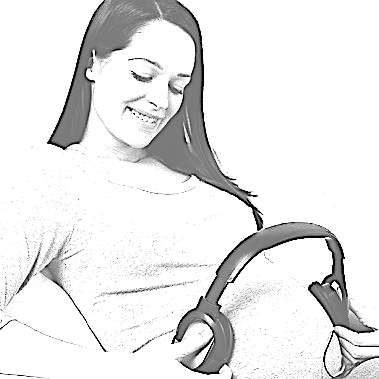
\includegraphics[scale=0.28]{../img/prenatale.png}
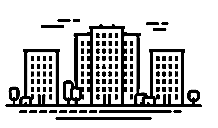
\includegraphics[scale=0.55]{../img/metro.png}
\end{center}
\end{itemize}

An example of the dichotomy just described can be found in analyzing the pitches of a melody.

To accomplish this we must activate several cognitive mechanisms which, in their simplest form are:

\begin{itemize}
\tightlist
\item processing the melodic profile (the progression of the ups and downs)  \(\rightarrow\) occurs more easily in both children and adults, with or without musical experience or literacy.
\item processing musical intervals (the distance between pitches) \(\rightarrow\) occurs less easily in general and to a greater extent in individuals with more experience or musical literacy (\href{http://www.musicaecodice.it/gitmedia/emc/1_media/veloso.mp3}{melody}).
\end{itemize}

\subsection{Re-compose a puzzle}\label{re-compose-a-puzzle}

\begin{center}
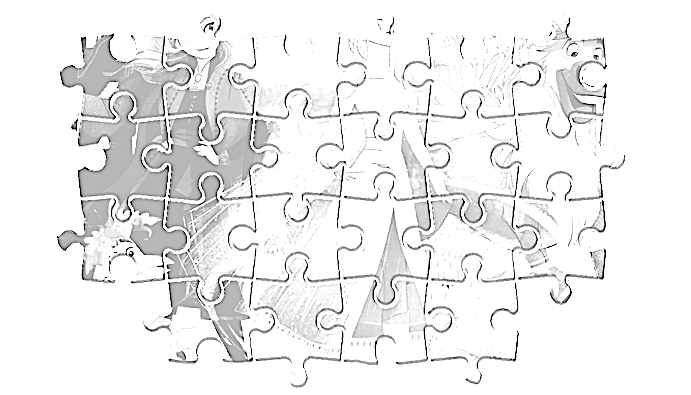
\includegraphics[scale=0.3]{../img/puzzle.png}
\end{center}

Re-constructing an image.

An abstract thing reconstructed in the physical world through a sequence of actions.

\begin{itemize}
\tightlist
\item we continuously interact between abstract and real world through attempts to correctly reproduce the original image.
\item we can reproduce the process many times but we cannot consider them copies.
\item we can't modify it.
\item it does not require necessary linguistic representation but cognitive skills.
\item during the re-composition process it need time and space but when the process is ended it need only space (in the case of a musical reproduction a space in our memory and consciousness).
\end{itemize}

This has to do with music representations, interpreters, players and performers.

Up to now we have thought about sound, music and their perception but not about the actors involved in the process of making music.

\begin{itemize}
\tightlist
\item composer.
\item interpreter.
\item listener.
\end{itemize}

We will delve deeper into these concepts in a dedicated paragraph \textit{Forms of human expression}.

\section{Music's meanings }\label{musics-meanings}

When we talked about the semantic level we mentioned the meaning but\ldots what is the meaning of music and what does music represent for humans?

We start again with sound waves \(\rightarrow\) it represent music in the physical world like clouds or mountains.

This has to do with both perceptual and cognitive processes.

By abstraction we can consider sound waves as \href{http://www.musicaecodice.it/gitmedia/emc/1_media/segno1.mp4}{signs}.

Let's think on these topics: 

\begin{itemize}
\tightlist
\item their production, transmission and interpretation. 
\item the ways in which something is communicated and signified. 
\item the production of symbolic objects.
\end{itemize}

\subsection{Signs and sounds }\label{signs-and-sounds}

\begin{center}

\includegraphics[scale=0.45]{../img/montagne.png}
\end{center}

\begin{itemize}
\tightlist
\item let's go hiking
\item we're driving on a mountain road.
\item we see cars parked on the side of the road.
\item we realize that the mountain path we're looking for probably starts there.
\end{itemize}

We can consider the many parked cars a sign that indicated the beginning of the trail.

Our intentions, the context, and the tracks we encountered along the way activated within us an action-reaction mechanism made up of perceptions, expectations, emotions, interpretations, etc.

We can define:

\begin{itemize}
\tightlist
\item the sight of the group of cars \(\rightarrow\) the signifier (plane of expression) --- what made us understand something.
\item the presence of the beginning of the trail \(\rightarrow\) the signified (plane of content) --- what we understood.
\end{itemize}

Speaking semiotically the union of these two elements gives rise to a sign that generates an increase in knowledge.

Having found the beginning of the trail is what we can call the paradigmatic effect of the sign (we were looking for something and we found it).

Listen (\href{http://www.musicaecodice.it/gitmedia/emc/1_media/uccellini.mp3}{exemple 1}, \href{http://www.musicaecodice.it/gitmedia/emc/1_media/bach_1.mp3}{exemple 2}, \href{http://www.musicaecodice.it/gitmedia/emc/1_media/berio.mp3}{exemple 3}) and answer.

\begin{enumerate}
\def\labelenumi{\arabic{enumi}.}
\tightlist
\item what kind of information do they provide us?
\item what is the signified content of these acoustic expressions?
\item what kind of increase in knowledge was achieved after listening to them?
\end{enumerate}

These short sound texts could refer to three classic genres of electroacoustic music: soundscape composition, computer music and tape music.

All are carried by sound waves but have profoundly different signified contents that cannot be deduced (or composed) starting from the acoustic parameters of the sound.

\subsection{Composers, players and listeners }\label{composers-players-and-listeners}

\begin{center}

\includegraphics[scale=0.6]{../img/nuvole.png}
\end{center}

Come back to the mountain path.

\begin{itemize}
\tightlist
\item we're walking on the path.
\item the clouds are gathering \(\rightarrow\) signifier.
\item we understand that it's about to rain \(\rightarrow\) signified.
\item we decide to come back to the car \(\rightarrow\) practical effect.
\end{itemize}

Signs often have a practical effect.

Sounds often have a practical effect (hearing thunder is like seeing clouds).

Have music pratical effect?

Signs connect: 
\begin{itemize}
\tightlist
\item something perceptual \(\rightarrow\) the sight of cars or clouds with 
\item something cognitive \(\rightarrow\) the presence of the path or impending rain.
\end{itemize}

Signs are not signifiers \(\rightarrow\) their perception by someone is.

A sign is not something that represents something else.

It represent the relationship someone establishes between two elements:

\begin{itemize}
\tightlist
\item a perceptible dimension (the view of the clouds). 
\item  an intelligible dimension (we connect it to the possibility of rain).
\end{itemize}

This relationship: 

\begin{itemize}
\tightlist
\item occurs \textit{a posteriori}.
\item is not necessarily intentional on the part of the sender (clouds are not harbingers of rain, just as the person who parked on the side of the road didn't mean to tell us the start of the trail).
\end{itemize}
We can connect signifier and signified only through an experiential factor (previously, when we saw those clouds, it rained).

\begin{center}
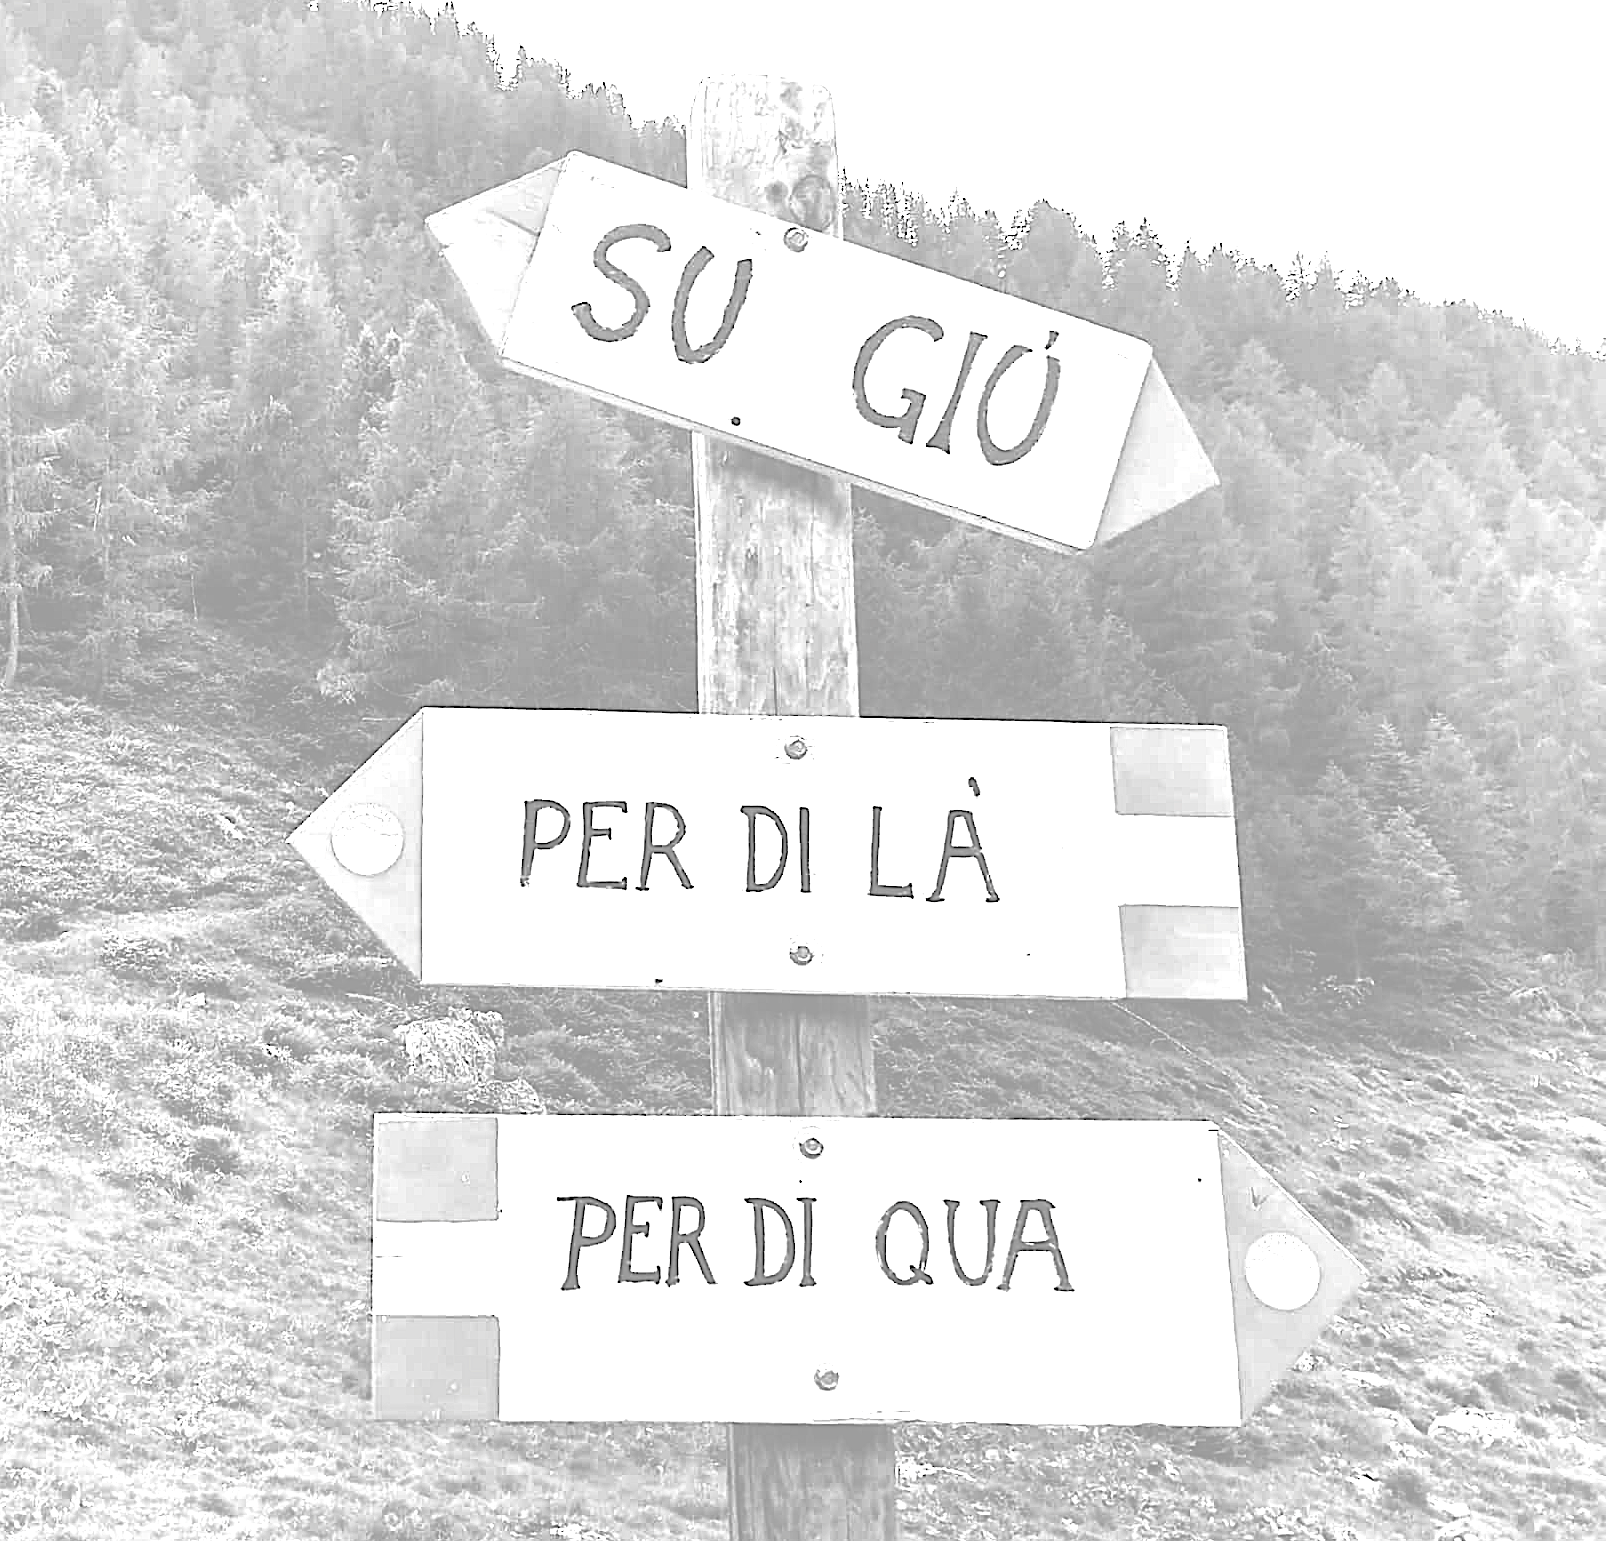
\includegraphics[scale=0.4]{../img/cartello.png}
\end{center}

Signification \(\rightarrow\) as the examples just given, we are constantly surrounded by a multiplicity of unconsciously produced signs.

All these signs have the potential to become signifier expressions if interpreted by a recipient in the general act we can define as signification.

Communication \(\rightarrow\) the sign is voluntarily produced by the emitter to convey a message, such as the signs in the previous image or the same images within this text.

Listen (\href{http://www.musicaecodice.it/gitmedia/emc/1_media/annuncio.mp3}{exemple 1}, \href{http://www.musicaecodice.it/gitmedia/emc/1_media/pubbli.mp3}{exemple 2}, \href{http://www.musicaecodice.it/gitmedia/emc/1_media/ligeti.mp3}{exemple 3}) and answer.

\begin{itemize}
\tightlist
\item what is the practical effect of the three sound texts?
\item is sound information contained in the acoustic properties of the sound texts?
\end{itemize}

Sounds can be both signification and communication.

Music can be only comunication.

In the performing arts of non-oral traditions (such as the western musical tradition), things get even more complicated because several actors play in the communication process:

\begin{itemize}
\tightlist
\item composer \(\rightarrow\) usually thinks of a composition in his mind (symbolic musical language) and then represent it through some kind of notational code on a score.
\item score \(\rightarrow\) the coded instructions needed by an interpreter to reproduce the composer's ideas in the physical world in the form of sound waves.
\item interpreter \(\rightarrow\) must know both the musical language used by the composer and the symbolic language through which it was codified (semiography).
\item listener \(\rightarrow\) receiver that interprets an interpretation.
\end{itemize}

In acoustic music it is always like this, while in electroacoustic music things can change.

\subsection{Do you know this music? }\label{do-you-know-this-music}

\begin{center}
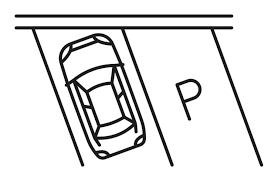
\includegraphics[scale=0.4]{../img/parcheggio.png}
\end{center}

What is the relationship between signifiers and signifieds activated bythe receiver based  on?

Is this relationship always valid and somehow implicit in the signifier, or does it depend on context and conditions?

Let's consider the example of clouds and rain.

There is no an universal law that says that every time there are clouds in the sky, it will rain.

The relationship is established through `a posteriori' inductive generalization codified in an interpretative rule \(\rightarrow\) it often rained after observing clouds in the sky, and therefore, whenever we encounter clouds, we associate them with the phenomenon.

Does this also apply to the example of cars parked on the side of the road?

In this case:

\begin{itemize}
\tightlist
\item there isn't an universal law according to which every time we observe parked cars, a mountain path is nearby.
\item there isn't an interpretative rule established by inductive generalization, since parked cars rarely indicate the start of a trail.
\end{itemize}

The way of reasoning that led to the signification (inference) was induced:

\begin{itemize}
\tightlist
\item by the contingent dimension \(\rightarrow\) place and context.
\item by the affective dimension \(\rightarrow\) enthusiasm for the hike, desire to find the trail to start walking, etc.
\item by the reference culture, or that set of knowledge, value systems, habits, and behaviors within which we live and which have almost naturally led us to that conclusion and not another.
\end{itemize}

The cognitive inferences used daily in our interpretations are not entirely personal or subjective \(\rightarrow\) are based on precise codes.

These codes:

\begin{itemize}
\tightlist
\item are formal systems that transcend individual choices, often imposing the use of certain mental categories.
\item are not universal.
\item are more or less lasting stabilizations of collective ways of thinking, acting, desiring, and preferring.
\item are dictated, maintained, and modified by social pressure.
\item are social and cultural customs, interpretative habits that take on the appearance of a law (without actually being one).
\end{itemize}

If we hadn't shared the same culture and been part of the same society with the many people who parked their cars on the day of the excursion, that sign simply wouldn't exist.

The sign isn't in things or ideas, but in the forms of their relationship.

Listen (\href{http://www.musicaecodice.it/gitmedia/emc/1_media/miles.mp3}{exemple 1}, \href{http://www.musicaecodice.it/gitmedia/emc/1_media/rameau.mp3}{exemple 2}, \href{http://www.musicaecodice.it/gitmedia/emc/1_media/gamelan.mp3}{exemple 3}) and answer.

Describe the differences between the three sound texts: 

\begin{itemize}
\tightlist
\item what is the first information that comes to mind when you listen? 
\item what kind of information is? 
\item are there differences between the linguistic systems used in the three sound texts? \item if there are any, what information do they influence?
\end{itemize}

Some of these arguments lead us to understand sound signs as a cultural phenomenon and not merely acoustic since from this point of view the signifier coincides with the signified.

\subsection{Do you like this music?}\label{do-you-like-this-music}

\begin{center}
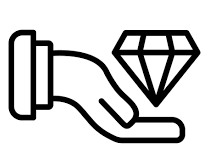
\includegraphics[scale=0.4]{../img/valore.png}
\end{center}

The above codes are anthropological conventions.

The relationships between expressions and content are connected to values, preferences, and tastes, all of which are extremely complex and are:

\begin{itemize}
\tightlist
\item arbitrary \(\rightarrow\) when viewed from the outside.
\item undisputed \(\rightarrow\) when viewed from the inside.
\end{itemize}

A sign arises through difference when a sensorial discontinuity materializes, such as when, while driving along a mountain road, we encounter parked cars.

The perceptual gap brings to the surface something significant, important, which we value by distinguishing it from other signs encountered along the way.

We value it in two ways:

\begin{itemize}
\tightlist
\item we are happy because we have found what we were looking for, namely, the opportunity to embark on a beautiful hike in the mountains.
\item we have achieved what we were seeking through a journey of knowledge that has kept our attention high (observing signs, the environment, other signs, etc.) and evaluating by comparing things (would it be better to stop at a restaurant or go for an hike?).
\end{itemize}

Social codes do not completely transcend individual choices but are linked to the ways in which the individual assumes them by mediating between collective and individual values.

In summary:

\begin{itemize}
\tightlist
\item value is what we aim for and what directs our series of actions and passions, giving precise meaning to each of them according to an implicit path.
\item value arises from the evaluative comparison of things, objects, and from the recognition of differences; the greater the evaluative comparisons along the path, the greater the value.
\item the continuous mediation between collective and individual values \hspace{0pt}\hspace{0pt}generates changes in anthropological codes.
\end{itemize}

Let's see a \href{http://www.musicaecodice.it/gitmedia/emc/1_media/sordi1.mp4}{video}.

\subsection{Texts and narratives}\label{texts-and-narratives}

\begin{center}
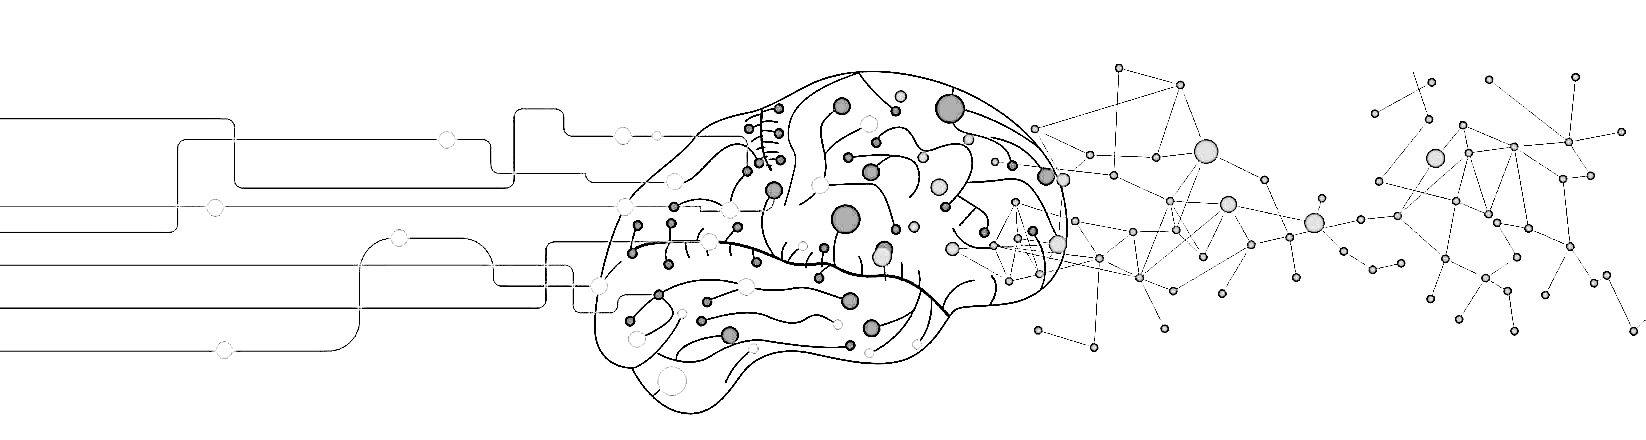
\includegraphics[scale=0.75]{../img/neuro.png}
\end{center}

The sign is just an iceberg tip.

It works because:

\begin{itemize}
\tightlist
\item it breaks down into many small, interrelated elements.
\item it composes larger entities by relating to other similar signs.
\end{itemize}

The parked cars signify the discovery of the path because:

\begin{itemize}
\tightlist
\item their unusual number in that place.
\item the way they are parked on the edge.
\item they thicken as they approach the path and then thin out.
\item they are in that place and not somewhere else.
\item they take on value thanks to differential relationships with other signs.
\item we are looking for the beginning of the path and not something else.
\item all these and other elements are part of a story that unfolds in a precise period of time.
\item this narrative is seen through a specific value-based, cultural, and anthropological perspective (a mountain hike).
\item we are in a specific emotional state (positive tension generated by the anticipation of being able to begin something we enjoy).
\item
  \ldots{}
\end{itemize}

The relationships established between these elements in a narrative generate the code through which that signifier refers to that probable meaning and not to another, forming what we might call a dynamic text.

Signs function because they are intertwined in texts.

The words of a language are like signs:

\begin{itemize}
\tightlist
\item the variable result of constant relationships between smaller elements (morphemes, phonemes, sound features),
\item themselves entities that compose larger structures (sentences, texts, speeches).
\end{itemize}

Every larger element capable of meaning transcends the smaller elements.

The meaning of a sentence transcends the meaning of the individual words that compose it, as well as the individual phonemes.

Texts are not just books, documents, etc., but any portion of the world with:

\begin{itemize}
\tightlist
\item determined limits (context).
\item precise internal articulation (code).
\end{itemize}

that carries some configuration of meaning, or better yet, a signification.

Do you remember the puzzle?

In order for meaning to:

\begin{itemize}
\tightlist
\item be produced.
\item be circulated.
\item be received.
\item be transformed.
\end{itemize}

it must refer to texts or units of meaning that various societies, historical periods, and cultures use to define their core values.

Let's see a \href{http://www.musicaecodice.it/gitmedia/emc/1_media/storia1.mp4}{video}.

\section{Forms of human expression}\label{forms-of-human-expression}

We can summarize the concepts just presented by following the thoughts of the musicologist J.J.Nattiez set out in his text `Music and discourse'.

Forms of human expression (including music) can be defined as symbolic forms only if we recognize three levels:

\begin{itemize}
\tightlist
\item poietic dimension (emitter) \(\rightarrow\) the set of strategies activated by the author that lead to the creation of the work (something that did not exist before).
\item aesthesic dimension (receiver) \(\rightarrow\) the set of strategies activated by the listener during the perception of the work.
\item the work itself (neutral) \(\rightarrow\) the text with its own internal organization that can be analyzed independently from the poietic and aesthesic dimensions.
\end{itemize}

\begin{center}
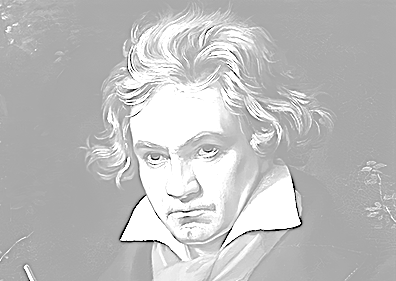
\includegraphics[scale=0.45]{../img/beethoven.png}
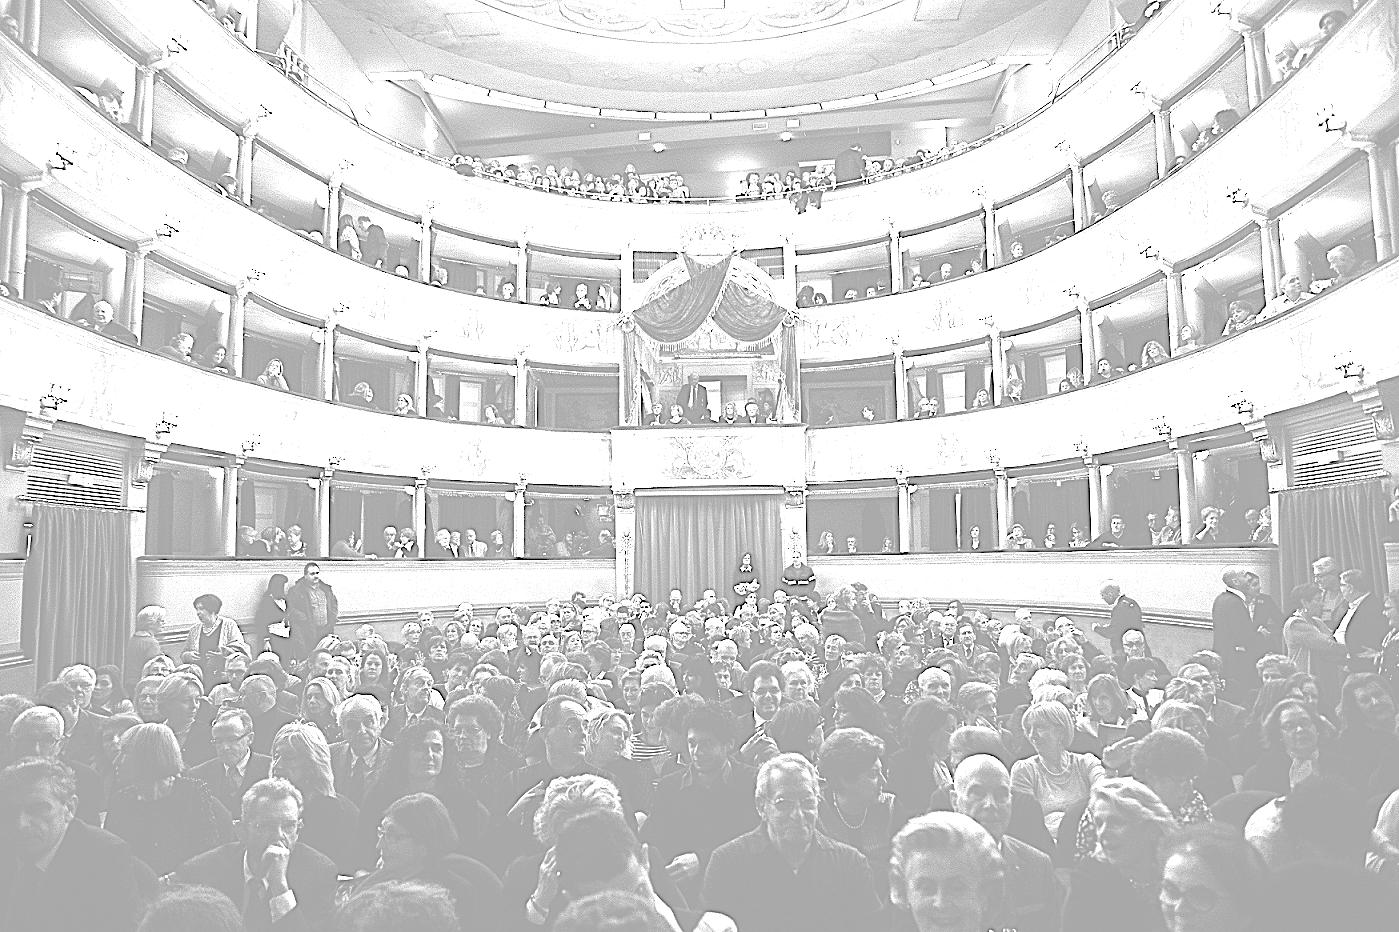
\includegraphics[scale=0.4]{../img/pubblico.png}
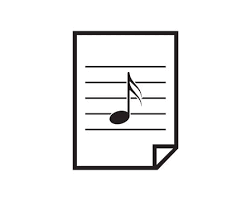
\includegraphics[scale=0.4]{../img/score.png}
\end{center}

\subsection{Poietic dimension}\label{poietic-dimension}

Active process of construction by the emitter (composer) of interpretant signs.

Each sign does not refer directly to an object but makes use of the intermediary action of a second sign which is its interpretant in a process of multiple references.

\begin{center}
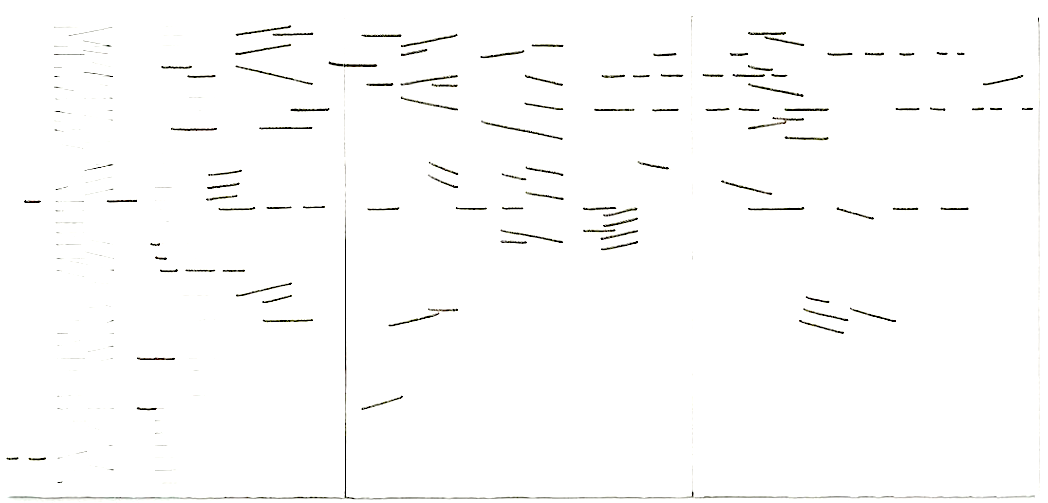
\includegraphics[scale=0.45]{../img/rimandi.png}
\end{center}

For example, in verbal language, if we write a word like table, we have:

\begin{itemize}
\tightlist
\item created a graphic sign (grapheme - formed by a sequence of letters and defined by its own rules) that, if
\item correctly interpreted by the reader, will cause him or her to pronounce the corresponding word (morpheme - sequence of phonemes defined by its own rules). If
\item correctly interpreted by the hearer, it will refer to a general idea of a table (an abstract concept defined by conventions derived from collective experience). If
\item correctly interpreted by someone, it will connect it to a real, meaningful table (object - defined by subjective experience).
\end{itemize}

This is true for a single word.

The interpretative signs become infinite when individual words are organized into a language.

Ognuno sta solo sul cuor della terra trafitto da un raggio di sole: ed è subito sera

Let's try to imagine the same process in music and the amount of control the composer can have over the \href{http://www.musicaecodice.it/gitmedia/emc/1_media/goldberg.mp3}{sound information} he wants to transmit.

\subsection{Aesthesic dimension}\label{aesthesic-dimension}

Active process of construction by the interpretant.

Process of understanding that can be defined as sharing information on cultural operations typical of a human social group.

In the case of artistic languages, the interpretative signs attributed to the work by the emitter are not necessarily the same as those projected by the receiver because:

\begin{itemize}
\tightlist
\item they are modulated by the context in which the interprete perceives the work.
\item they are modulated by any discrepancy in period or cultural context between the emitter and the receiver.
\item the perception of a sonata in the Baroque era is presumed to be totally different from the perception of the same work today, as the historical, social, technological, and cultural contexts are significantly different.
\end{itemize}

\begin{center}
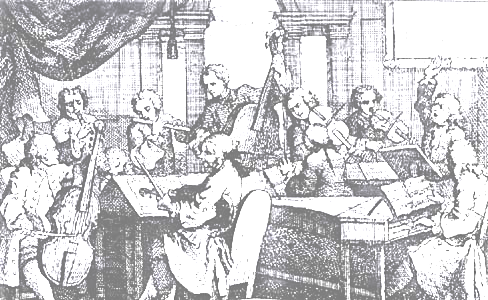
\includegraphics[scale=0.45]{../img/barocca.png}
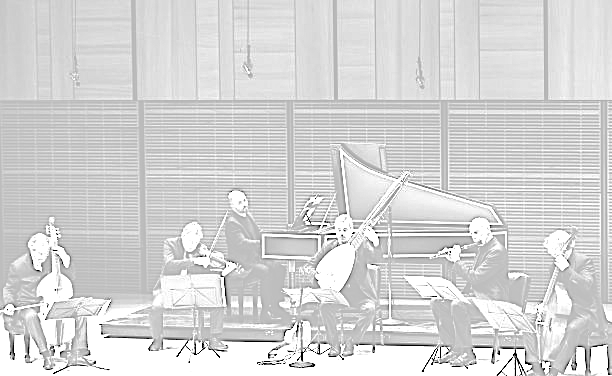
\includegraphics[scale=0.65]{../img/moderna.png}
\end{center}

The perception of a Beethoven symphony by an Amazonian native is totally different from ours, as is our perception of the microtones present in the \href{http://www.musicaecodice.it/gitmedia/emc/1_media/muezzin.mp3}{muezzin chants}.

\begin{center}

\includegraphics[scale=0.6]{../img/indigeni.png}
\end{center}

Let's also think about the technological dimension: the perception of the same sound text in a live concert is different from the perception of its reproduction recorded by an electroacoustic system perhaps while we wait for the subway.

\begin{center}
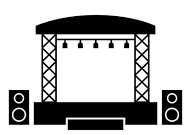
\includegraphics[scale=0.5]{../img/acousma.png}

\includegraphics[scale=0.5]{../img/sony.png}
\end{center}

\subsection{The work itself}\label{the-work-itself}

Regarding the understanding of the sound text itself Nattiez advocates the need to analyze: 

\begin{itemize}
\tightlist
\item works and styles as cultural and anthropological objects. 
\item harmony, rhythm, meter and all aspects that have a similar function in the grammar of natural language (comparison).
\end{itemize}

When we speak of grammars of musical parameters we are not referring exclusively to the analysis of the formal and structural characteristics of a specific musical text. We must also take into consideration the grammars of musical parameters generalized and historicized in styles and forms.

\begin{center}
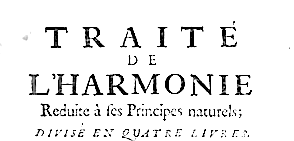
\includegraphics[scale=0.45]{../img/trattato.png}
\end{center}

Nattiez borrows from the study of verbal language the semantic exercise of breaking down meaning according to the use of words, which in music corresponds to the analysis of a melodic profile or a rhythmic system, or the distribution of harmonic fields in a tonal system or twelve-tone series, etc.

\begin{center}
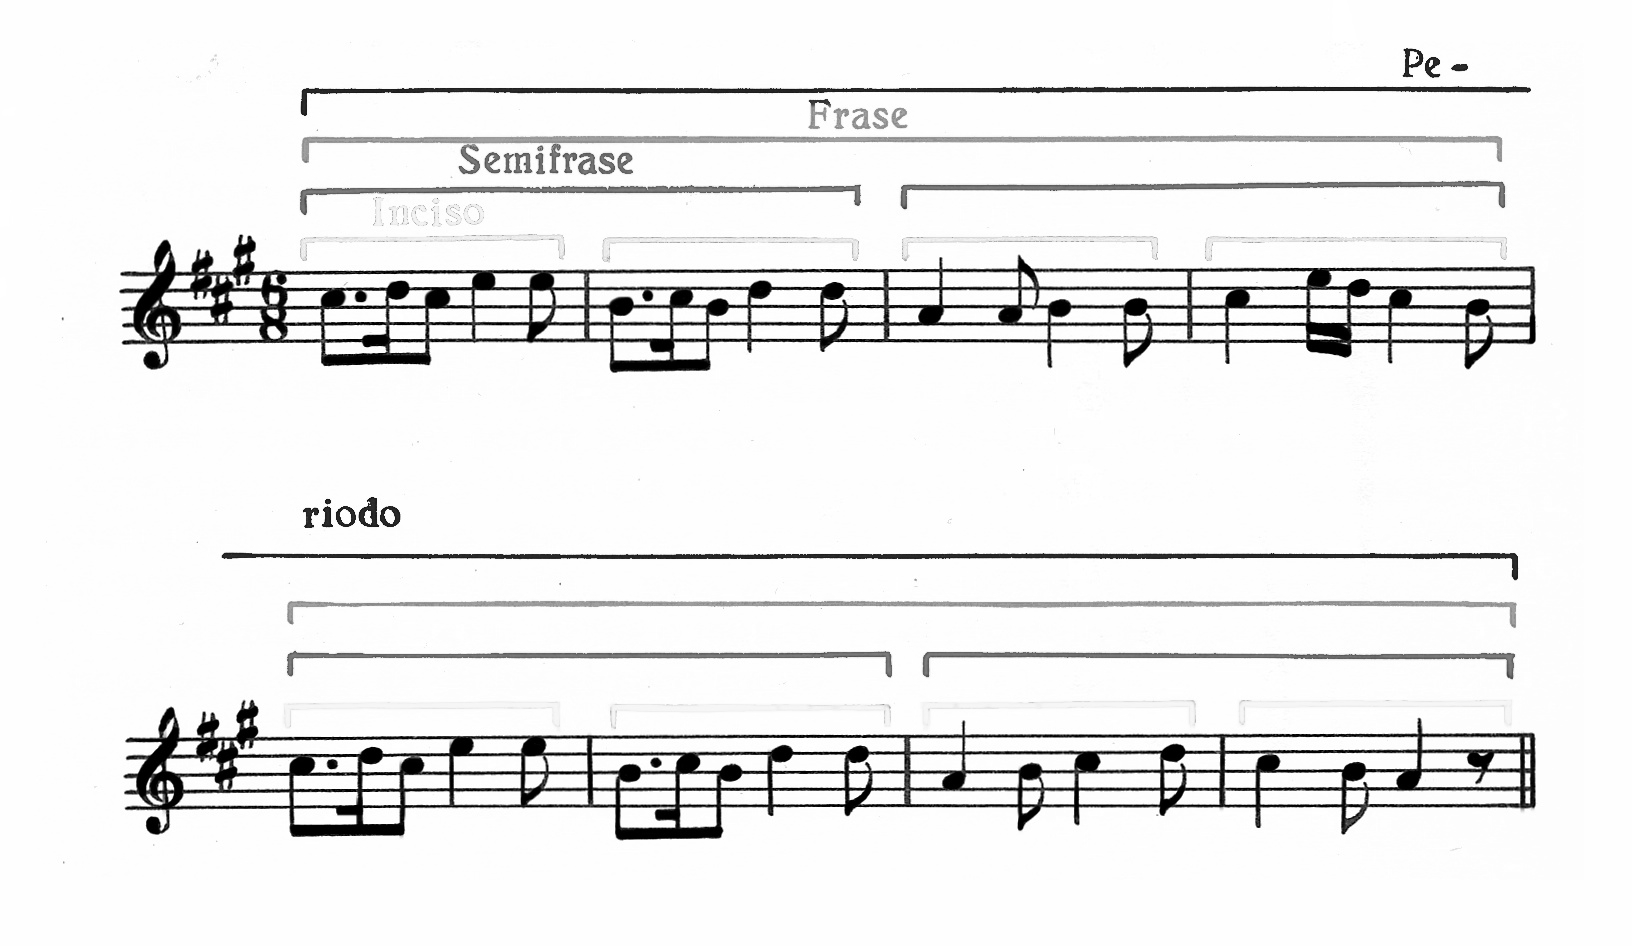
\includegraphics[scale=0.85]{../img/frasemus.png}
\end{center}

Each musical element (pitch, intensity, duration, timbre) can be separated and taken as a strategic variable in the production of a \href{http://www.musicaecodice.it/gitmedia/emc/1_media/quinta.mp4}{musical work}.

Ending, for Nattiez constructing a musical theory is the organization of a selection of interpretants adopted within an anthropological context.

Anyone who wants to invent a new musical grammar (a practice that has been widespread among art music composers since the 1950s) must take this into account and not just the definition of rules internal to the text.

Works do not exist in isolation since it is their place in history that provides their meaning and possible interpretations over time.

\begin{center}
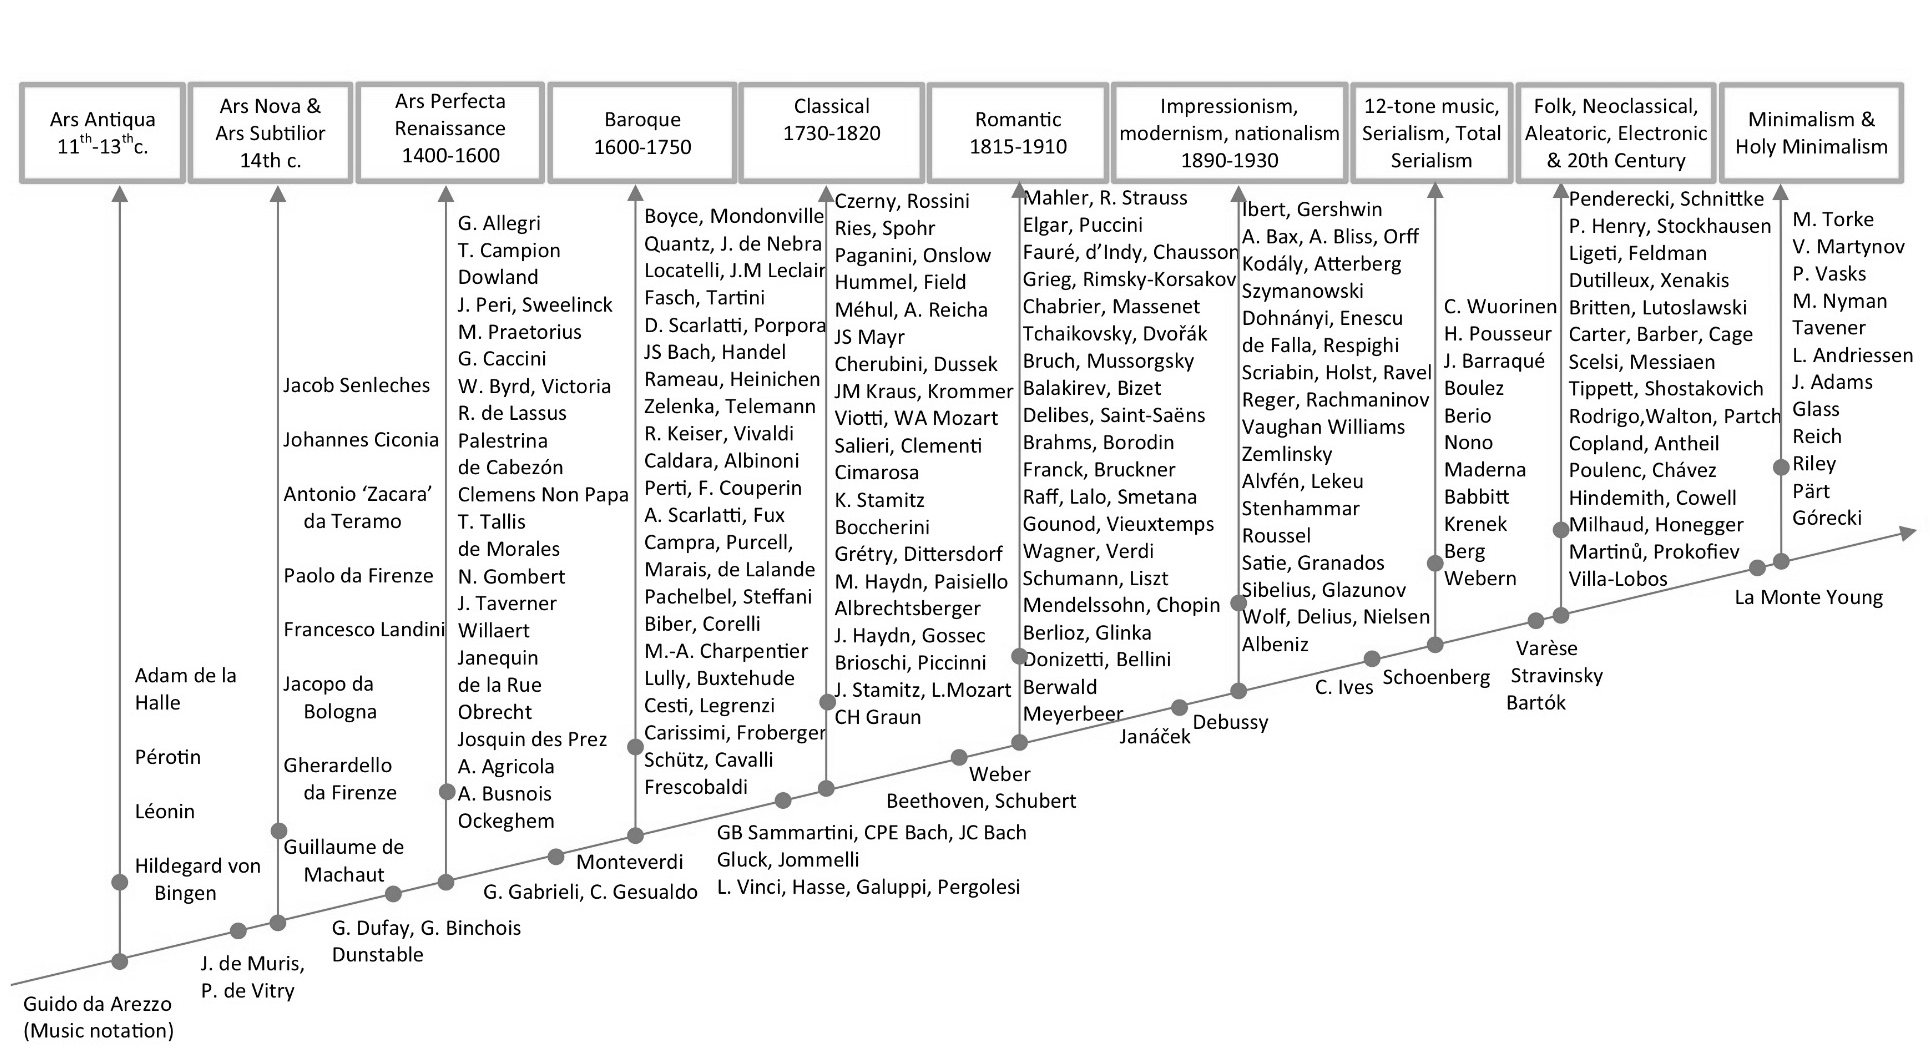
\includegraphics[scale=1]{../img/lineatempo.png}
\end{center}

The sound text can live a life of its own and be isolated from the the emitter but not from the anthropological context in which it was created and/or reproduced.

\subsection{Final reflections}\label{final-reflections}

Everyday life is filled with more or less voluntary signification.

Signification is the amniotic fluid within which human beings live.

We can highlight it and clarify its mechanisms.

This task is often hidden in everyday life.

For example, if we ask someone why they like a piece of music or a dress they will probably answer:

\begin{itemize}
\tightlist
\item because it's beautiful.
\item because it excites me.
\item because it's right.
\item because\ldots{}
\end{itemize}

Meaning often hides behind other motivations that tend to suppress it.

Let's think about written and spoken language.

In using it, we put into practice extremely complex knowledge that we tend to be unable to explain.

We would hardly be able to fully explain all the grammatical, phonetic, morphological, and syntactic rules we apply daily.

Language is practical knowledge that we almost never reason about (unless we are professional linguists).

Our daily experience works the same way: it appears random, spontaneous, and immediate.

In reality it is based on a dense and constantly changing network of relationships between things, people, places, etc.

Also the act of composing a piece of music should develops in the continuous passage from awareness of linguistic mechanisms (intelligence) to creativity.

Let'see a \href{http://www.musicaecodice.it/gitmedia/emc/1_media/senso1.mp4}{video}.
\chapter{Genres, instruments and tools}

\section{Genres}\label{genres}

Before starting to write an electroacoustic piece we should:

\begin{itemize}
\tightlist
\item define the instrumentation to be used which can include acoustic instruments, electroacoustic instruments, virtual instruments or a mix of these types.
\item define the sound amplification and diffusion system.
\end{itemize}

%\begin{center}
%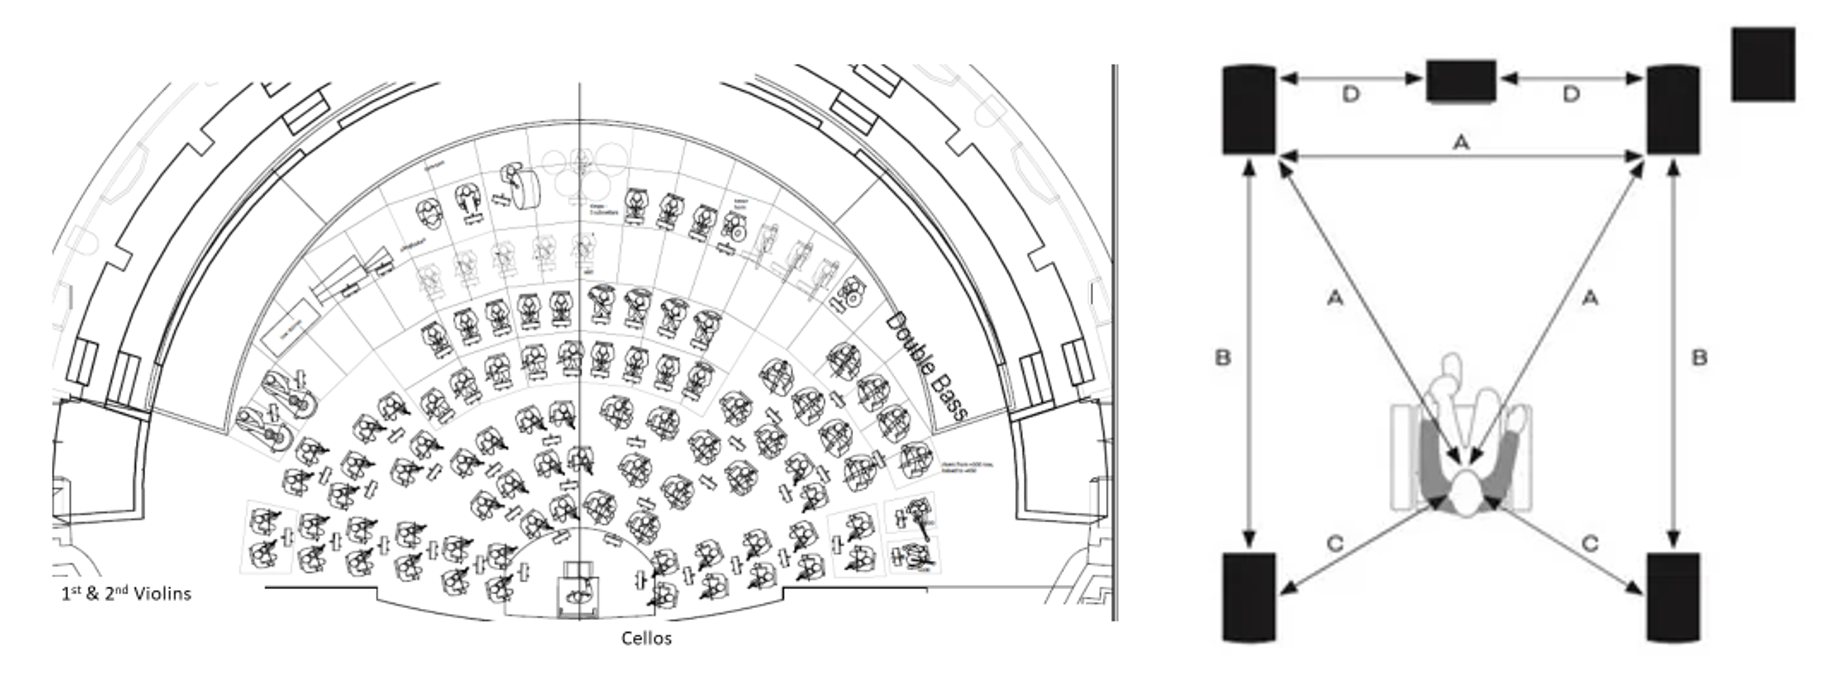
\includegraphics[scale=0.9]{img/dispo.png}
%\end{center}

For this reason here we categorize the different types and genres of electroacoustic music by dividing them into two macro areas defined by the way of controlling sounds and musical parameters.

\begin{itemize}
\tightlist
\item non interactive systems.
\item interactive systems.
\end{itemize}

We will explore the compositional strategies of each in dedicated chapters.

\section{Non interactive systems}\label{non-interactive-systems}

This category includes genres that:

\begin{itemize}
\tightlist
\item don't involve any human interaction during the performance.
\item involve interactions that don't influence the musical or sound text in any way.
\end{itemize}

According with the reflections of the previous chapter we can affirm:

\begin{itemize}
\tightlist
\item interactions may influence the listener's perception of the sound text (mainly through the different characteristics of the diffusion systems used).
\item interactions don't change the sound text.
\end{itemize}

This category can be divided into two further subcategories:

\begin{itemize}
\tightlist
\item fixed media music.
\item live sequencing.
\end{itemize}

The image shows the possibles audio chains in this category.

\begin{itemize}
\tightlist
\item non-real-time sound processing.
\item non-real-time synthesis.
\item real-time synthesis.
\end{itemize}

\begin{center}
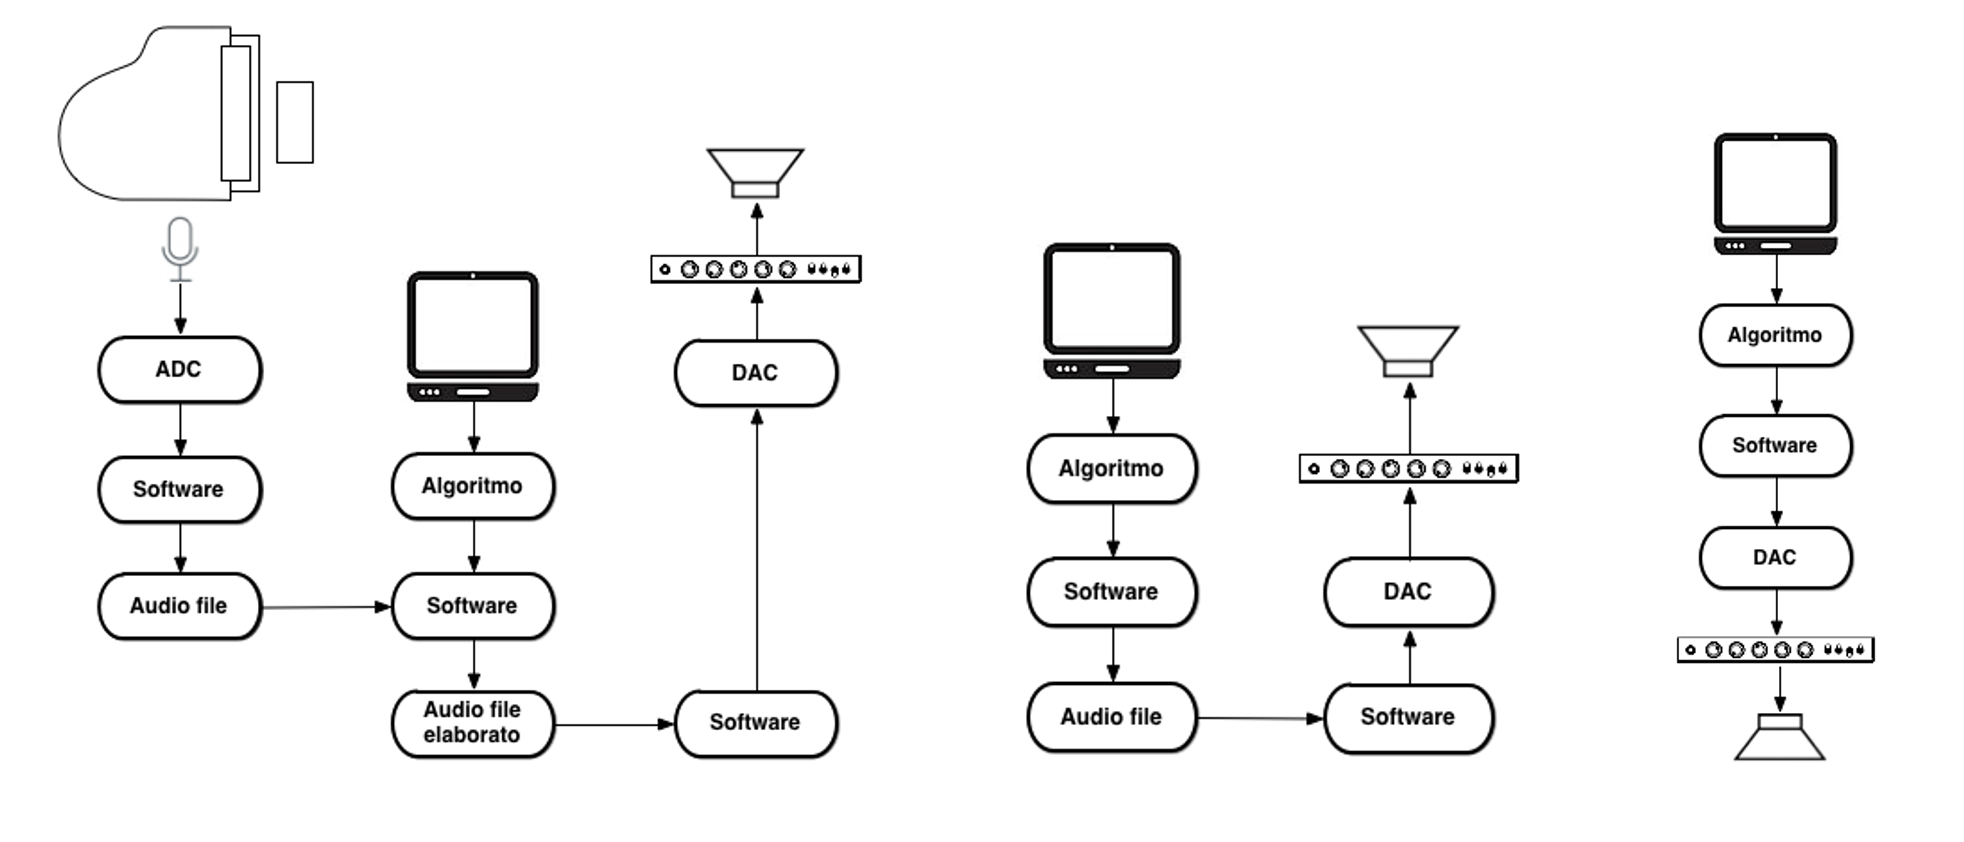
\includegraphics[scale=1]{../img/chains.png}
\end{center}

\subsection{Fixed media music }\label{fixed-media-music}

This subcategory denotes music or video that is played back from a recording.

This used to be called `tape music' but tapes are no longer used.

The entire work is stored on a single medium and reproduced from beginning to end.

We can identify three main genres:

\begin{itemize}
\tightlist
\item acousmatic music.
\item wallpaper music, ambient music and soundscapes.
\item radiodrama.
\end{itemize}

\subsubsection{Acousmatic music }\label{acousmatic-music}

\begin{center}
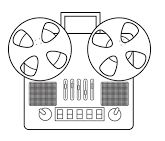
\includegraphics[scale=0.5]{../img/tape.png}
\end{center}

We can start from \textit{musique concrète}.

In the 1940s Pierre Schaeffer began composing with the sound (acoustic world).

After applying various sound elaborations (editing, filtering, reversal, etc.) he began to apply musical techniques to their combinations (repetition, transposition, reordering, etc.) inventing new musical structures (symbolic world).

In doing so, he reversed the compositional practice that had been in force for centuries in the Western musical tradition.

The listeners could not make the cognitive associations illustrated in the first chapter.

They activating exclusively the basic cognitive mechanisms common to all human beings.

This listening mode has been called \textit{reduced listening}.

All listeners of this new music are comparable to the aborigine who listens to a Beethoven symphony.

P.Shaeffer - \href{http://www.musicaecodice.it/gitmedia/emc/2_media/shaeffer.mp3}{Etude aux chemins de fer} for tape (1948) - extract.

\begin{itemize}
\tightlist
\item mono analog tape.
\item recorded and processed train sounds.
\item sounds from the acoustic environment.
\item we can recognize the sound source and its processing.
\item perceived as a distortion of reality.
\end{itemize}

Acousmatic music is the modern evolution of musique concrète.

By the mid-1970s a number of composers felt a need to designate their conception clearly in terms of specific methodology, syntax, and tools.

François Bayle suggested adopting the term acousmatique.

This term comes from the Greekakousma: what is heard.

Students of Pythagoras listened to his teachings from behind a screen unable to see him.

He believed that the lack of visual cues would force his students to focus all their attention on his message.

After his death his followers split into:

\begin{itemize}
\tightlist
\item acousmatics (practitioners of the mystic doctrine)
\item mathematics (scientists).
\end{itemize}

The loudspeaker was the modern equivalent of the screen partition.

\textit{"From an esthetical point of view acousmatic music concentrates on the poetical and spectral richness of sounds, and plays with this very particular characteristic of sound hearing in which the perception of anacoustic phenomena is associated with its cause; hence the perception of a sound whose cause is unknown or unrecognizable for our perception, induces the listener to imagine non-existing causes and to perceive
music as a complex creative phenomena in which musical sense and musical sounds have to be interpreted simultaneously, with generally very little relation with our perceptive reality. The question is not to find out how sounds are made but how their combination will generate imaginary perceptions of imaginary realities in our mind."}

Teruggi, D. 1995. What about acousmatics? In Journal of Electroacoustic
Music. Vol. 7. London: Sonic Arts Network

\href{http://www.musicaecodice.it/gitmedia/emc/2_media/teruggi.pdf}{More info}

B.Parmegiani - \href{http://www.musicaecodice.it/gitmedia/emc/2_media/parmegiani.mp3}{De Natura Sonorum} for tape (1975) - extract.

\begin{itemize}
\tightlist
\item stereo digital tape.
\item recorded and processed sounds plus synthetic sounds.
\item sounds from an imaginary environment.
\item we cannot recognize the sound source.
\item perceived as an alternative or virtual reality.
\end{itemize}

Another characteristic of acousmatic music is that it is performed live on loudspeaker orchestras (acousmonium).

Indeed Bayle referred to acousmatic musica as \textit{"art of projected sounds which is shot and developed in the studio, projected in a hall, like cinema".}

H.Vaggione - \href{http://www.musicaecodice.it/gitmedia/emc/2_media/vaggione.mp3}{Consort}. for convolved violins (2011) - extract.

\begin{itemize}
\tightlist
\item multitrack digital file.
\item recorded and processed instrumental sounds.
\item sounds from music environment.
\item we can recognize the sound source and its avatars.
\item perceived as a piece of music.
\end{itemize}

\href{http://www.musicaecodice.it/gitmedia/emc/2_media/space.pdf}{More info} about acousmatic works interpretation.

\subsubsection{Wallpaper music, ambient music and soundscapes }\label{wallpaper-music-ambient-music-and-soundscapes}

\begin{center}
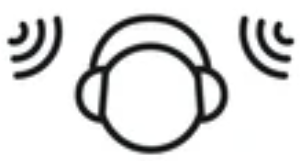
\includegraphics[scale=0.4]{../img/ambi.png}
\end{center}

We can start from Eric Satie (non-electroacoustic composer).

He was a precursor of minimalism, muzak, and many other 20th-century musical genres.

Satie conceived this musical genre as a backdrop to everyday activities (passive listening).

Satie was familiar with this idea due to its role as role as a Montmartre café pianist in the late 19th and early 20th century.

E.Satie - \href{http://www.musicaecodice.it/gitmedia/emc/2_media/satie.mp3}{Musique d'ameublement} (1917) for ensemble - extract.

\begin{itemize}
\tightlist
\item acoustic instruments.
\item pattern iteration.
\item music environment.
\item time dilation (psychological time).
\item passive and non immersive listening.
\item perceived as a piece of music.
\end{itemize}

We know well how nowadays we are bombarded daily by this type of music in a totally involuntary motion.

Let us recall what was stated in the first chapter on the basic cognitive mechanisms of human beings.

In the 1950s a visionary composer like J.Cage took this idea to its extreme with the piece 4'33'\,' whose sonic and musical content consists of the background noise of a finite time.

Later in 1978 another composer Brian Eno coined the term ambient as a musical genre.

A Sunday morning in the Cologne airport while waiting for a flight he tought: \textit{The light was beautiful, everything was beautiful, except they were playing awful music. They spend hundreds of millions of pounds\ldots on everything. Except the music.}

It was this that compelled him to begin composing music for public environments.

We must consider that the diffusion of sounds and/or music in environments not designed for active listening can change the perception of that environment in a subconscious way.

It is time that through sound redraws the boundaries of a space.

B.Eno - \href{http://www.musicaecodice.it/gitmedia/emc/2_media/eno.mp3}{Music for Airports} (1978) for tape - extract.

\begin{itemize}
\tightlist
\item stereo vynil. 
\item pattern iteration.
\item music environment. 
\item time dilation (psychological time). 
\item passive and semi immersive listening. 
\item perceived as a piece of music.
\end{itemize}

\href{http://www.musicaecodice.it/gitmedia/emc/2_media/eno.pdf}{More info}

Soundscape composition can represent a meeting point between musique concrete and ambient music because:

\begin{itemize}
\tightlist
\item it uses sound materials recorded from the real world or synthesized.
\item does not recompose them according to symbolic rules and principles into a musical form.
\item its purpose is to construct or reconstruct a real or virtual soundscape.
\end{itemize}

It's essentially based on the studies and works of Canadian musicologist and composer Raymond Murray Schafer.

To put it simply, we can say that different types of sounds coexist in a sound environment and we can identify three types:

\begin{itemize}
\tightlist
\item geophony \(\rightarrow\) all the sounds of nature of non-biological origin.
\item biophony \(\rightarrow\) all the sounds of nature of biological origin but not caused by humans.
\item anthrophony \(\rightarrow\) all sounds generated by humans.
  \begin{itemize}
  \tightlist
  \item language.
  \item music.
  \item mechanical sound.
  \end{itemize}
\end{itemize}

Schafer also divides the sounds of a soundscape into two categories:

\begin{itemize}
\tightlist
\item hi-fi \(\rightarrow\) all sounds that have an hight signal-to-noise ratio (they are distinguishable from the background noise).
\item lo-fi \(\rightarrow\) all sounds that have a low signal-to-noise ratio (they are indistinguishable from the background noise).
\end{itemize}

Three main elements in a soundscape:

\begin{itemize}
\tightlist
\item keynote \(\rightarrow\) sounds that most characterize an environment, analogous to the tonality in tonal music.
\item sound signals \(\rightarrow\) all the foreground sounds that do not necessarily characterize an environment but may appear occasionally.
\item soundmark \(\rightarrow\) The unique sounds of a given soundscape.
\end{itemize}

N.Barret - \href{http://www.musicaecodice.it/gitmedia/emc/2_media/soundwalk.mp3}{Soundwalk} (1998) - extract.

\begin{itemize}
\tightlist
\item stereo digital tape. 
\item no pattern. 
\item acoustic environment. 
\item time as in real life (clock time). 
\item passive and immersive listening. 
\item perceived as an acoustoc environment.
\end{itemize}

\href{http://www.musicaecodice.it/gitmedia/emc/2_media//schafer.pdf}{More info}

\subsubsection{Radiodrama }\label{radiodrama}

\begin{center}

\includegraphics[scale=0.5]{../img/radio.png}
\end{center}

Radio drama can use only four kinds of signs:

\begin{itemize}
\tightlist
\item speech.
\item sound effects.
\item music.
\item silence.
\end{itemize}

Any one of these by itself can be a very slippery client to deal with.

Silence cane a listener suspect a transmission failure and switch off or tune over to another on.

Sound effects are notoriously misleading - a sneeze can be taken for a bomb explosion!

An unfamiliar music will sound irritatingly like cacophony.

And speech says nothing to someone who doesn't know what you mean by the words.

But if you hit on harmonious combination of the right choies of these four kinds you can move mountains, deploy infantry battalions with Air Force support, immerse a soul in the joys of paradise.

In short do anything you please, all in few minutes one after another.

The main focus is narrativity and a continuous balance in the construction of meaning between explicit sounds (both in natural and auditory language) and perceptual hints and/or allusions.

O.Wells - \href{http://www.musicaecodice.it/gitmedia/emc/2_media/wells.mp3}{War of the worlds} (1938) - extract.

\begin{itemize}
\tightlist
\item mono radio signal.
\item natural language.
\item didactic sound design to simulate the real acoustic environment.
\item time as in real life (clock time).
\item active listening non immersive.
\item perceived as a representation of reality.
\end{itemize}

\href{http://www.musicaecodice.it/gitmedia/emc/2_media/radio.pdf}{More info}

\subsubsection{Computer music - algorithmic composition}\label{computer-music---algorithmic-composition}

\begin{center}
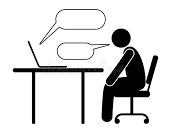
\includegraphics[scale=0.5]{../img/comp.png}
\end{center}

The birth of computer music is naturally linked to the invention of the electronic calculator and the subsequent spread of personal computers as well as the invention of new (formal) languages that allow humans to communicate with these machines.

Starting from the second half of the 1950s, two orientations emerged:

\begin{itemize}
\tightlist
\item the first one (developed mainly in Europe) deals with the digital coding of musical parameters (assisted composition, assisted musical analysis, etc.).
\item the second one (developed mainly in USA) deals with the digital coding of sound parameters (synthesis and processing).
\end{itemize}

In 1957 MUSIC I was created by Max Mathews in Bell Laboratories.

It was the first software for playing music from mathematical functions.

After MUSIC I, there were: MUSIC II, III, IV, V, MUSIC 360, and then C-sound and SuperCollider languages still used today.

The main sound synthesis and processing techniques used are:

\begin{itemize}
\tightlist
\item additive synthesis.
\item subctractive synthesis (filters).
\item FM (Frequency Modulation) synthesis.
\item granular synthesis.
\item analysis and resynthesis (FFT).
\item generative algorithms for:

  \begin{itemize} 
  \tightlist
  \item musical structures.
  \item timbres.
  \item pitches.
  \end{itemize}
\item remote control of computers (MIDI, OSC, HID).
\end{itemize}

As we all know, nowadays computer is the main musical instrument, like piano in the 19th century.

The term \textit{computer music} as an aesthetic category identifies the musical genre adopted by the pioneers from the mid-50s to the late 90s

J.Chowning - \href{http://www.musicaecodice.it/gitmedia/emc/2_media/chowning%20.mp3}{Stria}. (1977) - extract.

\begin{itemize}
\tightlist
\item stereo digital tape.
\item sonic environment.
\item sounds from imaginary environment (only synthetic sounds - FM).
\item time dilation (psychological time).
\item active listening.
\item perceived as a piece of computer music.
\end{itemize}

\href{http://www.musicaecodice.it/gitmedia/emc/2_media/max.pdf}{More info}

\subsection{Live sequencing}\label{live-sequencing}

This subcategory is almost identical to the previous one except for two aspects: 

\begin{itemize}
\tightlist
\item works can be generated in real time through algorithms (computer music). 
\item tracks are divided into different sound files triggered in real time (sound design for theatre and gaming).
\end{itemize}

\subsubsection{Sound design for performing arts or video }\label{sound-design-for-performing-arts-or-video}

\begin{center}
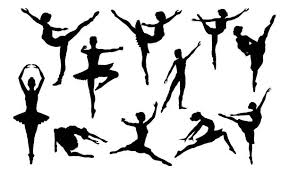
\includegraphics[scale=0.4]{../img/danza.png}
\end{center}

Works on fixed media which differ from the works illustrated in the previous section essentially for:

\begin{itemize}
\tightlist
\item sound does not have an absolute value but must be functional to dramaturgy.
\item divised into more or less short fragments.
\item open form \(\rightarrow\) fragments can be triggered in non-linear sequences (slightly different than what was said about random generation).
\item differenze musicali rispetto ai brani acusmatici.
\end{itemize}

Anonymous - \href{http://www.musicaecodice.it/gitmedia/emc/2_media/dance.mp3}{Dance!} (2010) - extract.

\begin{itemize}
\tightlist 
\item stereo digital tape. 
\item music functional to movement or dramatic timing.
\item secondary sensitive plane. 
\item passive listening. 
\item perceived as a complement to visual information.
\end{itemize}

\subsubsection{Sound design for gaming}\label{sound-design-for-gaming}

\begin{center}

\includegraphics[scale=0.3]{../img/game.png}
\end{center}

In this case too the sound must be functional to the game

It should:

\begin{itemize}
\tightlist
\item suggest a mood, evoke a feeling.
\item indicate a geographical locale.
\item define a character.
\item mirror or exaggerate how things sound in real life.
\item clarify the narrative
\end{itemize}

To simplify there are five sounds categories:

\begin{itemize}
\tightlist
\item dialogue \(\rightarrow\) any verbal speech in the game (player talk).
\item music \(\rightarrow\) any non-diegetic music (orchestral music).
\item sound Effects (Hard Effects) \(\rightarrow\) any sound from an real-life object (sounds of rocks falling).
\item foley \(\rightarrow\) any sound effect that the player makes (footsteps, etc.).
\item backgrounds (ambience) \(\rightarrow\) noise from the environment (wind, rain, etc.).
\end{itemize}

Procedural audio:

\begin{itemize}
\tightlist
\item sounfiles triggered by user actions.
\item real time shynthesis by internal oscillators.
\end{itemize}

Artistically we could merge game music, soundscape composition, acousmatic music and radiodrama.

Various - \href{http://www.musicaecodice.it/gitmedia/emc/2_media/gaming.mp3}{8 bit music}(1990) - extracts.

\begin{itemize}
\tightlist
\item stereo digital samples or real time oscillators.
\item music functional to gamer emotions.
\item also called procedural music.
\item pattern iteration.
\item music environment.
\item time dilation (psychological time).
\item non-immersive audio diffusion but immersive psychological function.
\item passive listening.
\end{itemize}

\href{http://www.musicaecodice.it/gitmedia/emc/2_media/gaming.pdf}{More info}

\section{Interactive systems }\label{interactive-systems}

This category includes genres that:

\begin{itemize}
\tightlist
\item involve human interaction during the performance as happens with acoustic instruments.
\item these interactions influence the musical or sound text at different levels.
\end{itemize}

Compared to the previous typology the presence of one or more performers significantly influences:

\begin{itemize}
\tightlist
\item the anthropological and contextualised perception of the musical action.
\item its representative nature.
\end{itemize}

This category can be divided into three further subcategories:

\begin{itemize}
\tightlist
\item hyper-instruments.
\item live set.
\item live coding.
\end{itemize}

The image shows the possibles audio chains in this category.

\begin{itemize}
\tightlist
\item real-time processing of pre-recorded or pre-synthesized sounds (parameters can be controlled through various types of devices - MIDI, OSC, HID, sensors).
\item real-time processing of signals captured through microphones or sensors (parameters can be controlled (parameters can be controlled in the previous modes but also through control signals derived in some way from the incoming audio signal).
\end{itemize}

\begin{center}
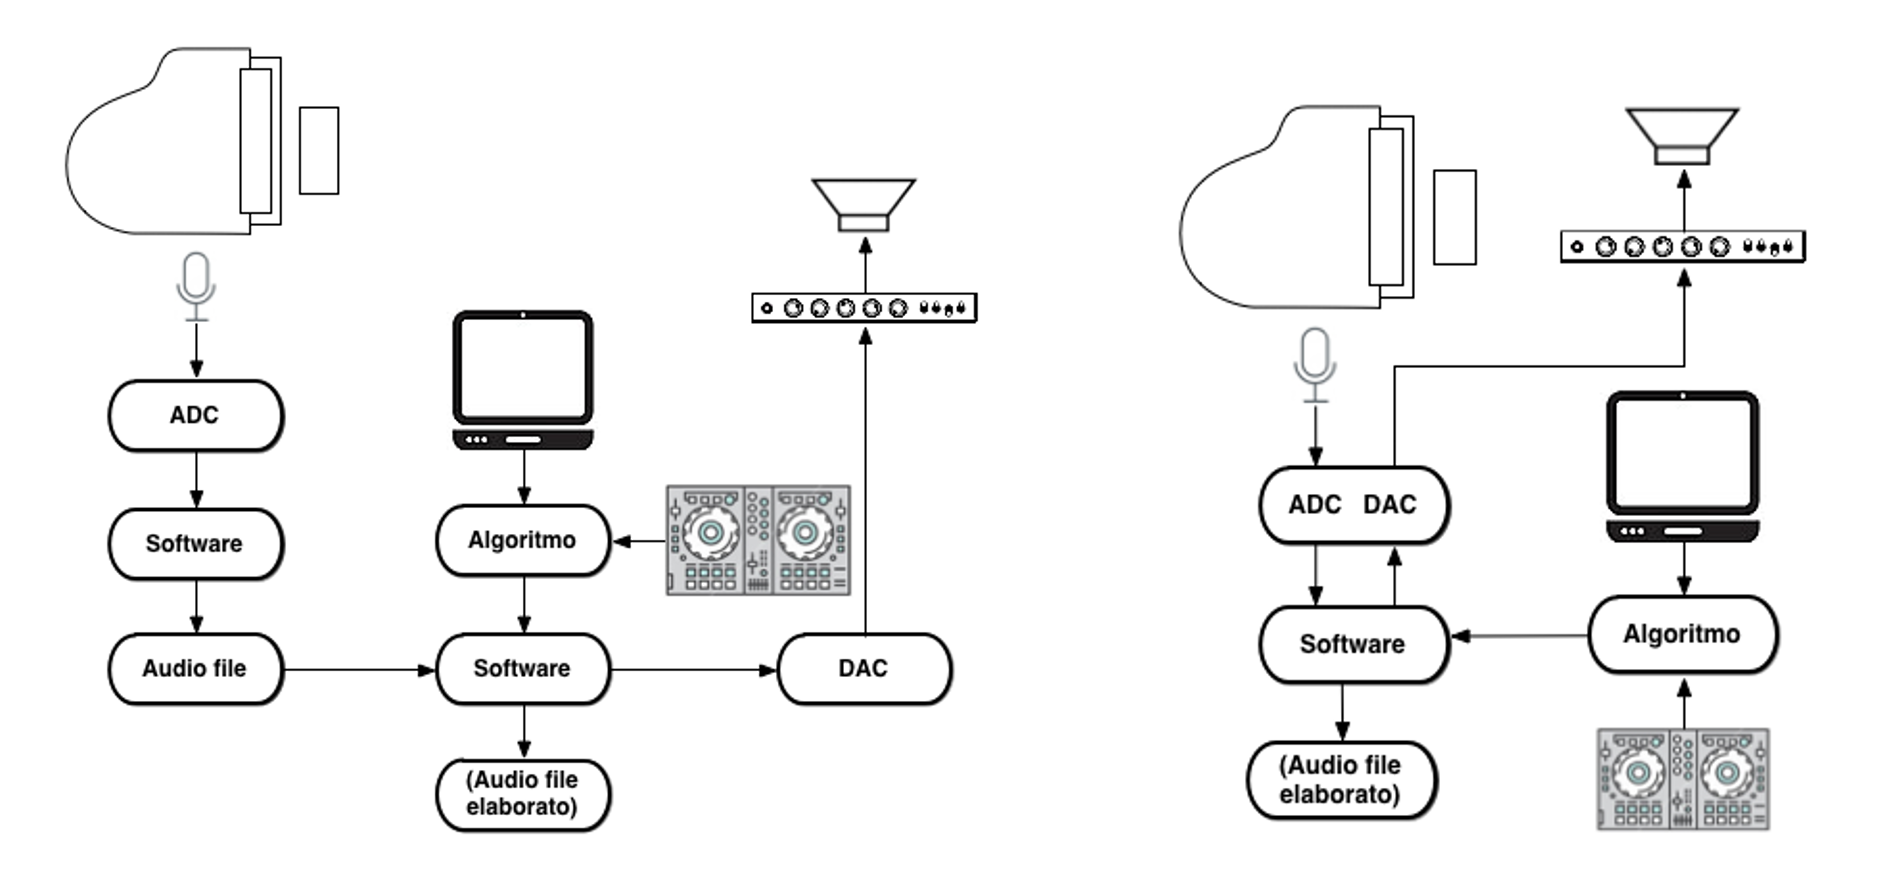
\includegraphics[scale=1]{../img/chain2.png}
\end{center}

\subsection{Hyper-instrument}\label{hyper-instrument}

\begin{center}

\includegraphics[scale=0.6]{../img/lel.png}\\
P.Boulez - \href{http://www.musicaecodice.it/gitmedia/emc/2_media/boulez1.mp4}{Anthèmes 2} (1994) - extract.
\end{center}

Augmented musical instrument that uses technology to extend the capabilities of a traditional instrument and enhance the performer's expressiveness.

Two types:

\begin{itemize}
\tightlist
\item real-time augmented instrumental techniques \(\rightarrow\) sound processes are controlled by:

  \begin{itemize}
  \tightlist
  \item an electronic performer who interacts with different types of controllers.
  \item by information extracted from the audio signal produced by the instrument itself (feature extraction as control signals).
  \end{itemize}
\item cyborg luthiery \(\rightarrow\) sound processing is controlled by movements and/or gestures of the performer captured by different types of sensors.
\end{itemize}

Three main goals:

\begin{itemize}
\tightlist
\item respond to the performer's input in a dynamic and expressive way allowing for a deeper connection between the musician and the music.
\item produce sounds and musical effects that are impossible to achieve with traditional instruments alone.
\item expanding musical forms.
\end{itemize}

\subsection{Live set }\label{live-set}

\begin{center}
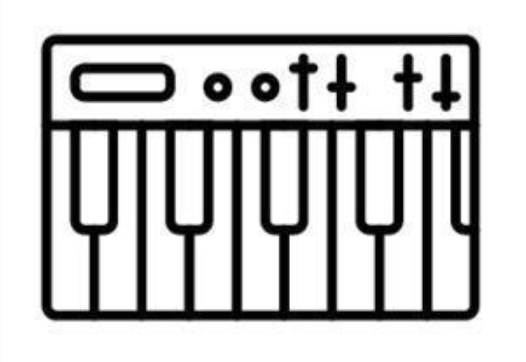
\includegraphics[scale=0.3]{../img/lset.png}\\
Slork - \href{http://www.musicaecodice.it/gitmedia/emc/2_media/slork1.mp4}{Twilight} (2013) - extract.
\end{center}

Live performance where songs are performed using analog or digital electronic musical instruments.

Often musicians improvise in a live set, making each performance unique.

Can be a solo performance or a laptop ensemble.

One of the most important aspects of this genre is to think about and assemble original performance environments which leads to the search for new human/machine interfaces dedicated to the generation of new sounds in the musical field.

\subsection{Live coding}\label{live-coding}

\begin{center}

\includegraphics[scale=0.4]{../img/lcod.png}\\
SuperCollider \href{http://www.musicaecodice.it/gitmedia/emc/2_media/livec1.mp4}{Live Coding} - extract.
\end{center}

Also called:

\begin{itemize}
\tightlist
\item on-the-fly programming.
\item just in time programming.
\item conversational programming.
\end{itemize}

Search for new musical forms, new places for performance and new audiences.

It is part of a larger artistic movement called creative coding.

If channeled into the Western musical tradition, we can think of it as a new version of organ improvisations in the Baroque era.

From a semiographic point of view the most interesting aspect is that the score is the code and is created and manipulated in real time.

The compositional process which has always belonged to the author's private sphere becomes public and an integral part of the performance itself (do you remember the first paragraphs of the previous chapter?).

\section{The virtual instrument paradigm}\label{the-virtual-instrument-paradigm}

In this section we define a virtual instrument model that will be useful in next chapters.

If anyone is unfamiliar with SuperCollider, they can download an introductory text at
\href{https://ccrma.stanford.edu/~ruviaro/texts/A_Gentle_Introduction_To_SuperCollider.pdf}{this
link}.

In the chapter on live electronics we'll make some small modifications to allow signal input.

\subsection{Software installation }\label{software-installation}

Download and install:

\begin{itemize}
\tightlist
\item \href{https://github.com/capital-G/sc_kernel}{sc\_kernel} (if you want to execute supercollider code in this notebook)
\item \href{https://supercollider.github.io/}{SuperCollider}
\end{itemize}

If you want to play SuperCollider from this notebook you have to select the textit{sc\_kernel}.

Instead, I recommend copying and pasting the code into the SuperCollider IDE Interpreter.

\subsection{Instrumental model}\label{instrumental-model}

Let's create a computer model that contains functions common to most virtual instruments (sound generators).

\begin{itemize}
\tightlist
\item an oscillator.
\item an amplitude envelope (with or without sustain).
\item a stereo panner.
\item a signal output.
\end{itemize}

We also establish the basic parameters we want to control dynamically (they will increase depending on the synthesis algorithm chosen).

\begin{itemize}
\tightlist
\item frequency (Hz).
\item general amplitude (0.0 to 1.0).
\item duration (seconds).
\item pan position (-1.0 to +1-0).
\item pan interpolation time (movements)
\item output bus.
\item trigger.
\item kind of voice allocation (doneAction:0 or 2).
\end{itemize}

\begin{center}
\includegraphics[scale=0.35]{../img/modello.png}
\end{center}

\begin{lstlisting}[frame=single] 
s.boot;
s.meter;
s.scope;
s.plotTree;
\end{lstlisting}

In SuperCollider we can define it with the `SynthDef' (synthesis definition) class.

This class contains the instructions (algorithms) needed to build multiple copies (instances) derived from the model.

\begin{lstlisting}[frame=single, caption=Instrument model] 
SynthDef.new(\model, {arg freq=500, amp=0, dur=1, pan=0, pantime(0.0), 
                          out=0, t_gate=0, done=2;
                      var sig, env;
                          sig = SinOsc.ar(freq);
                          env = Env.new([0.0,1.0,0.5,0.7,0],                
                                        [0.1,0.1,0.3,1.0].normalizeSum * dur,
                                        -4    
                                        );
                          env = EnvGen.kr(env, t_gate, doneAction:done);
                          sig = sig * env * amp;
                          sig = Pan2.ar(sig, pan.varlag(pantime));
                      Out.ar(out, sig)
                      }).add;        
\end{lstlisting}
Now we can generate as many instances as we want.

We have two ways to control the instance parameters.

They vary depending on the voice allocation we want.

\textbf{Dynamic voice allocation (poliphonic)} 

Instance self-destructs when the amplitude envelope expires (doneAction:2).

In this case we pass parameters at instantiation time (array of \textbackslash key, value).

\begin{lstlisting}[frame=single,caption=Dynamic voice allocation] 
Synth.new(\model, [\freq, rrand(890,1234), 
                   \amp, 0.5, 
                   \dur, rrand(0.1,2), 
                   \pan, rand2(1.0), 
                   \pantime, 0.1, 
                   \done, 2, 
                   \t_gate,1 ])
\end{lstlisting}

\textbf{Static voice allocation (monophnic)}

Two passages: 

\begin{itemize}
\tightlist
\item create instance and assign it to a variable.
\item send one or multiple parameter changes by \textit{set} method.

\begin{lstlisting}[frame=single, caption=Static voice allocation] 
a = Synth.new(\model, [\done, 0]);
a.set(\freq, rrand(890,1234), 
      \amp, 0.5, 
      \dur, rrand(0.1,2), 
      \pan, rand2(1.0), 
      \pantime, 0.1, 
      \t_gate,1)
\end{lstlisting}
\end{itemize}

Then we can kill it.

\begin{lstlisting}[frame=single] 
a.free;
\end{lstlisting}
Or kill all Synths on the Server.

\begin{lstlisting}[frame=single] 
s.freeAll;
\end{lstlisting}
The type of voice allocation is strictly linked to the type of amplitude envelope.

\textbf{With sustain (as in keyboards)}

There isn't a total duration.

In this case we must send a message of \textit{gate 1} (noteon) and then textit{gate 0} (noteoff).

\begin{lstlisting}[frame=single, caption=Instrument model with sustain] 
SynthDef.new(\sust, {arg freq=500, amp=0, pan=0, pantime(0.0), 
                     out=0, gate=0, done=2;
                     var sig, env;
                         sig = SinOsc.ar(freq);
                         env = Env.adsr;         
                         env = EnvGen.kr(env, gate, doneAction:done);
                         sig = sig * env * amp;
                         sig = Pan2.ar(sig, 0);
                     Out.ar(0, sig)
                     }).add;       
                                                
a = Synth.new(\sust, [\done, 0]); 
\end{lstlisting}
Send \textit{gate 1} (noteon)
\begin{lstlisting}[frame=single] 
a.set(\amp, 0.5, \gate, 1);
\end{lstlisting}
Send \textit{gate 0} (noteoff)
\begin{lstlisting}[frame=single] 
a.set(\gate, 0);
\end{lstlisting}
Kill the Synth.
\begin{lstlisting}[frame=single] 
a.free;
\end{lstlisting}

\textbf{Without sustain (as in percussion or plucked intruments)}

There is a total duration.

In this case we must send a gate message preceded by \textit{t\_}.

This produce an automatic \textit{gate 0} message after a time calculated on the specified duration

\begin{lstlisting}[frame=single, caption=Instrument model without sustain] 
SynthDef.new(\nosust,  {arg freq=500, amp=0, dur=1, pan=0, pantime(0.0), 
                            out=0, t_gate=0, done=2;
                        var sig, env;
                            sig = SinOsc.ar(freq);
                            env = Env.perc(0.1*dur,0.9*dur);                     
                            env = EnvGen.kr(env, t_gate, doneAction:done);
                            sig = sig * env * amp;
                            sig = Pan2.ar(sig, 0);
                        Out.ar(0, sig)
                        }).add;                                                   
a = Synth.new(\nosust, [\done, 0]);    // Create the Synth
\end{lstlisting}

Send \textit{t\_gate 1} (noteon + noteoff)

\begin{lstlisting}[frame=single] 
a.set(\amp, 0.5, \t_gate,1);
\end{lstlisting}

You can also trigger and kill it automatically.

\begin{lstlisting}[frame=single] 
a.set(\amp, 0.5, \done, 2, \t_gate,1);
\end{lstlisting}

Modifications to this model will be addressed in specific chapters.
\chapter{Fixed media}

\section{Historical framework}\label{historical-framework}

The first musical works recorded on media were created in the 1950s in the Radio France studios in Paris by composers belonging to the Groupe de recherches musicales (GRM) by Pierre Schaeffer.

Composers such as Pierre Henry, François Bayle, Bernard Parmegiani, Christian Zanési and Daniel Teruggi have collaborated with this institute.

These composers, more or less, referred to Schaeffer’s sound theories about "musique concrete" later outlined in his book  \textit{Traité des Objects Musicaux}.

The design of the studio followed strict Schaefferian theory and was completely centered around tape manipulation, recording and editing.

Two main electroacoustic instruments:

\begin{itemize}
\tightlist
\item phonogène \(\rightarrow\) a multi-headed tape instrument in three versions:
    \begin{itemize}
    \tightlist
    \item Chromatic phonogène. Tape loop at varied speeds. It produced short bursts of tape sounds at varying pitches defined by a small one-octave keyboard.
    \item Sliding phonogène. It produced continuous tone by varying the tape speed via a control rod.
    \item Phonogène Universal. It allowed time stretching without transposing the pitches and vice versa obtained through a rotating magnetic head.
    \end{itemize}
\item morphophone \(\rightarrow\)  a type of tape loop-delay mechanism. The sound was picked up at varying points on the tape by ten magnetic heads (one recording, one erasing and ten playback heads) then passed through ten bandpass fileters (one for each head).
\end{itemize}

Theories of musique concrète are based on the concept of a \textit{sound object}.

\section{Elements and strategies}\label{elements-and-strategies}

In this section we outline some concepts underlying any compositional process.

They are valid in subsequent chapters where we will explore the
specifics.

They are some of the main tools of composing electronic music.

\subsection{Sound objects}\label{sound-objects}

\begin{center}
\includegraphics[scale=0.4]{../img/sound.png}
\end{center}

Let's explore the concepts of sound object.

Pierre Schaeffer in his \textit{Traité des objets musicaux} (1966) wrote:

\textit{Let's assume a single microphone:}

\begin{itemize}
\tightlist
\item \textit{it is the point of convergence of all the soundwaves arriving from the sound points in the surrounding space.}
\item \textit{all the sound points in the initial space will be condensed into the microphone's membrane.}
\item \textit{the initial surrounding space is replaced by a sound point.}
\item \textit{if we play back it, it generates a new sound distribution in a new surrounding space.}
\item \textit{the diffusion medium (loudspeaker) is neutral favoring an acousmatic sound perception.}
\item \textit{we can consider this sound point as a word, a representation, not a recording of reality.}
\item \textit{we can call this representation a \textit{sound object}.}
\end{itemize}

A sound object is any sound phenomenon perceived:

\begin{itemize}
\tightlist
\item as a coherent whole.
\item heard in an acousmatic situation, regardless of its origin and meaning.
\end{itemize}

P.Henry - \href{https://github.com/musicaecodice/EMC/blob/main/3_fixed/suoni/henry.mp3}{Futuriste} for tape (1975)

\subsection{Objects, structure and form }\label{objects-structure-and-form}

\begin{center}
\includegraphics[scale=0.3]{../img/struc.png}
\end{center}

Schaeffer argues also that the object/structure pair is at the basis of our perceptual activity.

What is a structure?

A structure is a model the skeleton of a form.

What is a form?

General concept exposed by A.Lalande (Vocabulaire technique et critique de la philosophie):

\textit{Forms are sets, which constitute autonomous units, manifest an internal solidarity, and have their own laws.}

The nature of each element depends on the structure of the whole and the laws that govern it.

Neither psychologically nor physiologically does the element (object) pre-exist the whole.

The concept of form is therefore more complex than that of structure

Schaeffer illustrates this concept with two examples from western musical tradition:

\begin{itemize}
\tightlist
\item a melody cannot be reduced to the sequence of notes that compose it.
  \begin{itemize}
  \tightlist
  \item if when we listen to a melody we focus our attention on a single note, the perception of the melody vanishes.
  \item if we focus our attention on the entire melody (melodic profile) the perception of the individual notes vanishes.
  \end{itemize}
\item if the melody is in G major and we play an F natural we perceive a discordant note.

  \begin{itemize}
  \tightlist
  \item the musical scale is a structure that influences the encoding and decoding of the notes.
  \end{itemize}
\end{itemize}

Let us remember the continuous reference of the signs discussed in the paragraph about musical meaning.

Structure provides the relevant features that enable members of a musical tradition to encode and decode sounds.

In music, these structures are usually organized according to coherent variations of characterizing models (major, minor, etc.).

Schaeffer then aims to define a new sound vocabulary based on the intrinsic sound characteristics (morphosyntax) of sound objects.

Sound objects become musical objects.

\subsection{Musical objects}\label{musical-objects}

\begin{center}
\includegraphics[scale=0.2]{../img/texture1.png}
\end{center}

When we start to write a sound or musical work on a fixed media we should define few procedures:

\begin{enumerate}
\tightlist
\item choose and/or define the sound material (recorded or synthetic) to be used in the piece (sound objects).

  This choice should be made by:

  \begin{itemize}
  \tightlist
  \item recorded sound objects \(\rightarrow\) analysis of their morphological characteristics (perception).
  \item synthesized sound objects \(\rightarrow\) definition of their morphological characteristics (idea of a sound).
  \end{itemize}

  In both cases (analysis or definition) we can employ some simple strategies derived from the much more complex theories of composers and musicologists such as P.Schaeffer, M.Chion, D.Smalley and others.

  We should think about:

  \begin{itemize}
  \tightlist
  \item mass \(\rightarrow\) (spectral) quality that describes its perceived consistency, density, or \textit{weight}.
    \begin{itemize}
    \tightlist
    \item pure sound (sinusoid).
    \item tonic sound - defined pitch harmonic spectra (instrument).
    \item tonic group (chord or melodic pattern whitin a range).
    \item mixed sound (ambiguos).
    \item node (tremolo or ribattuto).
    \item nodal group (texture of inharmonic sounds).
    \item noise (white, pink, etc.).
    \end{itemize}
  \item
    matter \(\rightarrow\) grain - texture - object surface.

    \begin{itemize}
    \item smooth (static).
      \begin{center}  
      \includegraphics[scale=0.1]{../img/linea.png}
      \end{center}
    \item harmonica (trembling).
      \begin{center}
      \includegraphics[scale=0.45]{../img/tremore.png}
      \end{center}
    \item compact harmonica (fluctuating).
      \begin{center}
      \includegraphics[scale=0.1]{../img/scricchiolio.png}
      \end{center}
    \item compact (rustling).
      \begin{center}
      \includegraphics[scale=0.1]{../img/fruscio.png}
      \end{center}
    \item compact discontinuous (rhombus).
      \begin{center}
      \includegraphics[scale=0.2]{../img/rombo.png}
      \end{center}
    \item discontinuous (crackling).
      \begin{center}
      \includegraphics[scale=0.22]{../img/crepitio.png}
      \end{center}
    \item discontinuous harmonic (squeak).
      \begin{center}
      \includegraphics[scale=0.22]{../img/cigolio.png}
      \end{center}
    \item rhytmic (measured pattern).
      \begin{center}
      \includegraphics[scale=0.3]{../img/morse.png}
      \end{center}
    \end{itemize}
  \item dynamic.

    \begin{itemize}
    \tightlist
    \item global (dynamic profile) - if a sound object is fortissimo or piano or\ldots{}
    \item
      internal (grain envelopes) - dynamic evolution or contrast in internal parts.
    \end{itemize}
  \end{itemize}
  
  \begin{center}
  \includegraphics[scale=0.33]{../img/dyno.png}
  \end{center}

  Each of these parameters may or may not evolve over the course of the sound object in different ways:

  \begin{itemize}
  \item static (-) \(\rightarrow\) no evolution or small small fluctuations (tremolo, vibrato, beting, etc.).
    \begin{center}
    \includegraphics[scale=0.2]{../img/static.png}
    \end{center}
  \item opening (\textless) \(\rightarrow\) up glissando, crescendo, increase in density, etc.
    \begin{center}
    \includegraphics[scale=0.1]{../img/open.png}
    \end{center}
  \item closing (\textgreater) \(\rightarrow\) down glissando, diminuendo, decrease in density, etc.
    \begin{center}
    \includegraphics[scale=0.15]{../img/close.png}
    \end{center}
  \item alternated (\textless\textgreater) \(\rightarrow\) open and close like a pendoluum.
    \begin{center}
    \includegraphics[scale=0.22]{../img/alternate.png}
    \end{center}
  \item variated \(\rightarrow\) variation in pattern (rhythmic or melodic or spactral, etc.).
    \begin{center}
    \includegraphics[scale=0.35]{../img/varia.png}
    \end{center}
  \item random \(\rightarrow\) non evolutive.
    \begin{center}
    \includegraphics[scale=0.2]{../img/random.png}
    \end{center}
  \end{itemize}

  All these evolution can be fast or slow.
  
\item build a sound vocabulary (a sound palette) that includes one or more sets of sounds elaborated from those chosen in the previous point.

  The criteria adopted in generating this sound palette can be varied, including:

  \begin{itemize}
  \tightlist
  \item a set of coherent sound objects with morphological similarity to the original.
  \item a set of sound objects with gradual differentiation (direction, interpolation, etc.).
  \item a set of incoherent sound objects where the sound processing distort the original morphology.
  \end{itemize}

  The sound objects included in these sets become \textit{musical objects}  because they have acquired a semantic function within a system (such as the division of the octave into intervals of a scale in Western music theory).

\item order (compose) these sounds over time into different types of sound textures and paths, designing a musical form.

  The criteria we can adopt in doing so can include among others:

  \begin{itemize}
  \tightlist
  \item staticity - evolution - variation.
  \item continuity - discontinuity.
  \item contrast - uniformity.
  \item etc.
  \end{itemize}
\end{enumerate}

In this way we can construct and formalize an abstract thought.

Let's try to recognize musical objects, their characteristics and how they evolve over time in these extracts from B.Parmegiani works (\href{http://www.musicaecodice.it/gitmedia/emc/3_media/parme1.mp4}{extract1}, \href{http://www.musicaecodice.it/gitmedia/emc/3_media/parme2.mp3}{extract2}, \href{http://www.musicaecodice.it/gitmedia/emc/3_media/parme3.mp3}{extract3}).

\subsection{Time courses and musical forms}\label{time-courses-and-musical-forms}

Some further thoughts regarding time courses and musical forms.

In the figurative arts (architecture, painting, sculpture) forms exist in the dimension of space.

\begin{center}
\includegraphics[scale=0.4]{../img/scultura.png}
\end{center}

Musical forms are created over time.

\begin{center}
\includegraphics[scale=0.2]{../img/metronomo.png}
\end{center}

We cannot think of time in forms but only as events with different temporal courses.

\begin{center}
\includegraphics[scale=0.3]{../img/corsie.png}
\end{center}

A musical form can be defined as a thought that thinks about the course of events.

\begin{center}
\includegraphics[scale=0.7]{../img/pianoroll.png}
\end{center}

In the temporal domain (and therefore in the musical domain) there are two main formal typologies:

\begin{itemize}
\tightlist
\item teleo-logical.
\item circular.
\end{itemize}

\textbf{Teleo-logical time}\label{teleo-logical-time}

This time-course is goal-oriented and plays a dominant role in Western music.

The mode of a \href{http://www.musicaecodice.it/gitmedia/emc/3_media/finalis.mp3}{medieval melody} is determined by the finalis which is the last event of the course.

In tonal harmony a dissonance tends toward \href{http://www.musicaecodice.it/gitmedia/emc/3_media/risolvi.mp3}{resolution} just as a cadence moves toward the closing tonic.

Over a longer time an opera or the movements of a symphony gravitate towards the Finale (micro and macro structure).

Tonality based on \href{http://www.musicaecodice.it/gitmedia/emc/3_media/aggregati.mp3}{harmonic functions} has a teleo-logical nature as the sound aggregates are constantly moving towards reference points.

A point-to-point movement.

Only at the end when we reach the final cadence \href{http://www.musicaecodice.it/gitmedia/emc/3_media/forma1.m4v}{the process of the whole} being formed into a figure temporally accomplished.

\textbf{Circular time}\label{circular-time}

Movement returns incessantly to itself; it has no goal, no beginning, and no end.

In Western music, it appears:

\begin{itemize}
\tightlist
\item in the dissolution of functional harmony (early 1900) - \href{http://www.musicaecodice.it/gitmedia/emc/3_media/mal.mp3}{exemple}.
\item in phenomena of the serial or stochastic pointillistic form (mid 1900) - \href{http://www.musicaecodice.it/gitmedia/emc/3_media/web.mp3}{exemple}.
\item in phenomena of the anvantgarde and experimental music (after 1950) - \href{http://www.musicaecodice.it/gitmedia/emc/3_media/mont.mp3}{exemple}.
\end{itemize}

Music is de-teleologized and de-temporalized, eliminating any defined profile.

Thought that considers the process frees itself from the chains that bind it to hierarchies and the need to strive toward a goal.

A typical position of Eastern philosophies, thought seeks to free itself from all limitations to achieve the unity of being.

The concept of time in music has always historically stemmed from a general reflection.

For this reason, today we can choose which temporal typology to adopt to best construct the desired musical form.

\subsection{The poietic dimension: determinism}\label{the-poietic-dimension-determinism}

In the previous chapter we saw that the musicologist J.J.Nattiez defines the poietic dimension as the set of strategies activated by the author that lead to the creation of the work (something that did not exist before).

As for the simple organization of sounds over time, stripped of all other components that contribute to their creation, the processes we can employ in design and implementation are essentially two types:

\begin{itemize}
\tightlist
\item deterministic procedures.
\item stochastic procedures.
\end{itemize}

We will deal with the first type in this paragraph while the second in the next chapter on computer music.

In philosophical and scientific language, determinism is a conception according to which the events of metaphysical, physical, or moral reality are necessarily and invariably connected to each other.

If we make this choice when composing a piece, we face two options:

\begin{itemize}
\tightlist
\item use our \textit{libero arbitrio} and choose all the parameters at our own discretion (not randomly, but according to a specific intention).
\item follow or create systems of rules to generate or transform some or all of the parameters.
\end{itemize}

\textbf{Libero arbitrio}\label{libero-arbitrio}

This procedure may seem the simplest.

In reality it is the most complex because it cannot be formalized.

Its success depends exclusively on the composer's determination and experience.

It requires a high level of consciousness.

It presupposes a full awareness of oneself and the external world with which we interact, our identity and the complexities of our internal activities.

This is because the conveyance of the musical idea cannot by definition be governed by rules shared by:

\begin{itemize}
\tightlist
\item composer. 
\item performer. 
\item listener.
\end{itemize}

If we choose this procedure we must be careful to avoid any mnemonic reference to any musical systems.

It is a-thematic and a-motivic in the form of an infinite ever-changing continuous line.

Without developments, perceptible variations, or repetitions.

It is perhaps the procedure closest to pure unmediated expression.

We can consider it the ultimate point of arrival in the historical development of a musical civilization, absolute freedom understood not as a void but as a container of all possible rules.

\textbf{Rules and theories}\label{rules-and-theories}

The second option is to:

\begin{itemize}
\tightlist
\item choose a system of rules from a past or present musical tradition.
\item define our own system of rules that can be valid only for a single piece or a distinctive feature of our poetics.
\end{itemize}

The main difference is that in the first case the codes of meaning are shared within a reference culture while in the second they are not, or not yet.

Unlike in the past, today we can choose the system that best conveys our musical thinking because never before have our ears and senses been bombarded as continuously by every type of sound and language from the most disparate media as we are in our daily lives.

This idea is masterfully expressed in the appendix to some editions of I. Calvino's American Lessons, entitled \textit{Beginning and Ending}.

\textit{  {[}\ldots{]} Start writing a novel. }

\textit{And this is the moment of choice: we are offered the possibility of saying everything, in every possible way; and we must arrive at saying one thing, in a particular way.}

\textit{The starting point {[}\ldots{]} will therefore be this decisive moment for the writer: the detachment from the unlimited and multifaceted potentiality to encounter something that does not yet exist but that can exist only by accepting limits and rules.}

\textit{Up until the moment before we begin to write, we have the world at our disposal, a sum of information, experiences, values -- the world given as a whole, without a before or an after, the world as individual memory and as implicit potentiality; and we want to extract from this world a discourse, a story, a feeling: or perhaps more precisely we want to
perform an operation that allows us to situate ourselves in this world.}

\textit{We have all the languages at our disposal: those developed by literature, the styles in which civilizations and individuals have expressed themselves over the centuries and countries, and also the languages developed by the most varied disciplines, aimed at achieving the most varied forms of knowledge: and we want extract from it the
language suitable for saying what we want to say, the language that is what we want to say. {[}\ldots{]} }   

\section{Sound processing techniques in SuperCollider}\label{sound-processing-techniques-in-supercollider}

In this section we implement in SuperCollider some historical sound processing techniques controlled through deterministic procedures (scoring and sequencing).

Through these sound processing techniques we can define the sound palette (vocabulary) illustrated in point 2 of the previous paragraph.

We can divide them into two categories based on the characteristics of the oscillator type used:

\begin{itemize}
\tightlist
\item sampling. 
\item scratching.
\end{itemize}

In both cases we need to load the soundfiles into one or more buffers.

\subsection{Buffers}\label{buffers}

When we want to process a sounfile I suggest to use mono files.

Boot the audio system with few GUI.

\begin{lstlisting}[frame=single] 
s.boot;
s.meter;
s.plotTree;
\end{lstlisting}

Load a single soundile in one buffer.

\begin{lstlisting}[frame=single, caption=Load one sound file in a Buffer] 
b = Buffer.read(s, "/absolute/path/to/file.wav"); 
\end{lstlisting}

A best practice it's to include all the soundfiles in one folder providing the relative path.

It work only in SuperCollider IDE, not in Jupyter sc\_kernel.

\begin{lstlisting}[frame=single] 
"sounds/bach.wav".resolveRelative;
\end{lstlisting}

Some utility.

\begin{lstlisting}[frame=single] 
b.normalize; 
b.plot;      
b.play;      
\end{lstlisting}

Delete Buffer(s) from Server's memory.

\begin{lstlisting}[frame=single] 
b.free;     // one specific Buffer
s.freeAll;  // all Buffers
\end{lstlisting}

Load many sounfiles from a folder.

One soundfile \(\rightarrow\) one Buffer.

\begin{lstlisting}[frame=single,caption=Load many sounfiles from a folder] 
~paths = ("/absolute/path/to/folder" ++ "/*.wav").pathMatch; 
~bufs  = ~paths.collect{arg i; Buffer.read(s, i)};
\end{lstlisting}

We can then recall them by index (uditive monitor).

\begin{lstlisting}[frame=single] 
~bufs[1].play; 
\end{lstlisting}

Stopping audio:

\begin{itemize}
\tightlist
\item SuperCollider \(\rightarrow\) cmd + .
\item Jupyter sc\_kernel \(\rightarrow\) execute the cell below.
\end{itemize}

\subsection{Sampling }\label{sampling}

Let's define an instrument and the parameters we want to control:

\begin{itemize}
\tightlist
\item buffer to play.
\item start position.

  \begin{itemize}
  \tightlist
  \item absolute (0 to Buffer duration in seconds).
  \item relative (0 to 1).
  \end{itemize}
\item duration (seconds).
\item amplitude (0 to 1).
\item trasposition in semitones (float \(\rightarrow\) cents).
\item direction (1 \(\rightarrow\) recto -1 \(\rightarrow\) verso).
\item pan (-1 to 1).
\item trigger (without sustain).
\item doneAction (voice allocation type).
\end{itemize}

\begin{lstlisting}[frame=single, caption=Sampler model] 
SynthDef(\smp, {arg buf=0, pos=0, dur=0.2, amp=0, trsp=0, dir=1,p an=0,
                    t_gate=0,done=2;
                var sig, env;
                    sig = PlayBuf.ar(1, buf,     
                                     BufRateScale.kr(buf)*trsp.midiratio*dir,           
                                     t_gate,                                
		          BufSampleRate.kr(buf)* pos); // Absolute start position (frames) 
	         // BufFrames.kr(buf) * pos);    // Relative start position (0 to 1)
                    env = Env.linen(0.01,dur-0.02,0.01);                  
                    env = EnvGen.kr(env, t_gate, doneAction:done);
                    sig = Pan2.ar(sig * env * amp, pan);
                Out.ar(0,sig)
                }).add;
\end{lstlisting}

Test it.

\begin{lstlisting}[frame=single] 
Buffer.freeAll;
b = Buffer.read(s, "/absolute/path/to/file.wav");

Synth(\smp,[\buf, b, 
            \pos, 2.3, 
            \dur, 0.2, 
            \amp, 1, 
            \trsp, 0, 
            \dir, 1, 
            \pan, 0, 
            \done, 2, 
            \t_gate, 1])
\end{lstlisting}

\subsubsection{Sequencing}\label{sequencing}

We can define a sequence of parameter changes in the form of an Array and then dynamically recall it over time.

Next exemple has to do with \textit{libero arbitrio}: we can set all the parameters as we want.

\begin{lstlisting}[frame=single, caption=Deterministic sequencing] 
~tstr = 4.01; // Time stratching factor
~pos = [5.82, 9.11, 9.76, 0.39, 9.21, 2.85, 2.31, 0.05];       
~amp = [0.40, 0.65, 0.85, 1.00, 0.70, 0.50, 0.30, 0.10];
~dur = [1.40, 0.46, 1.18, 2.39, 0.69, 1.15, 3.41, 1.55]* ~tstr;
~trs = [1.40, 0.46, 2.18,-2.39, 3.69, 2.15,-3.41, 1.55];
~del = [1.48, 0.54, 2.41, 1.26, 3.07, 0.89, 1.16, 0.89]* ~tstr;
~dir = [1,      -1,   -1,    1,    1,   -1,    1,   1 ];
~pan = [-1,   -0.8, -0.6, -0.4,    0,  0.4,  0.6,   1 ];
~evt = ~del.size.postln; // Number of sonic events (notes)

r = Routine({ ~evt.do({arg id;                           
                         Synth(\smp,[\buf,b,
                                     \pos, ~pos[id], // index call
                                     \amp, ~amp[id],
                                     \dur, ~dur[id],
                                     \trsp,~trs[id],
                                     \dir,~dir[id],
                                     \pan,~pan[id],
                                     \done,2,
                                     \t_gate,1]);
		                 ~del[id].wait })
             }).play
\end{lstlisting}

Next example has to do with setting up deterministic rules.

The rule is cutting the soundfile in a defined number of cues and play it back with a defined time stratching.

\begin{lstlisting}[frame=single] 
~nfrag = 80;                // choose a number of cues
~dur   = b.duration/~nfrag; // compute fragment duration
~pos   = 0;                 // start position
~stch  = -0.08; // if > 0 = rest elif < 0 = superimposion (poliphony)

r = Routine({
            ~nfrag.do({
                    Synth(\smp,[\buf,b,
                                \pos, ~pos.postln,
                                \dur, ~dur,
                                \amp, 1, \trsp, 0, \dir, 1, \pan, 0,
                                \done, 2, \t_gate, 1 ]);
                    ~pos = ~pos+~dur; s// position increases at each step
                    (~dur+~stch).wait
	                })
            }).play
\end{lstlisting}

\subsubsection{Enveloping}\label{enveloping}

This technique consists in modifying the type of amplitude envelope of the original fragment.

We can do it in two ways:

\begin{itemize}
\tightlist
\item uniform \(\rightarrow\) one envelope type for all sonic events (grain).

  Here a percussive envelope.

\begin{lstlisting}[frame=single, caption=Percussive grain model] 
SynthDef(\grain, {arg buf=0, pos=0, dur=0.2, amp=0, trsp=0, dir=1, pan=0,
	                  t_gate=0, atk=0.1, done=2;
                  var sig,env;
                      sig = PlayBuf.ar(1, buf,
                               BufRateScale.kr(buf) * trsp.midiratio * dir,
                               t_gate,
                               BufSampleRate.kr(buf)* pos );
                     env = Env.perc(atk, dur-atk);
                     env = EnvGen.kr(env,t_gate,doneAction:done);
                     sig = Pan2.ar(sig * env * amp, pan);
                Out.ar(0,sig)
                }).add;
\end{lstlisting}

We can change dynamically attack time (0.01 to 0.99).

\begin{lstlisting}[frame=single] 
~durs = [0.79,0.68,0.57,0.46,0.25,0.14,0.23,0.32,0.41];       
~pos  = [1.1,2.3,0.5,3.7,1.9,2.1,0.3,3.5,2.7];
~atk  = [0.01,0.02,0.43,0.04,0.35,0.06,0.57,0.08,0.89];      

r = Routine({
            inf.do({arg item,id;  
                        Synth(\grain, [\buf, b, \amp, 1,
                                       \pos, ~pos.foldAt(id), // foldAt()
                                       \done,2, 
                                       \atk, ~atk.foldAt(id),
                                       \t_gate, 1]);
		                ~durs.foldAt(id).wait})
            }).reset.play
\end{lstlisting}

\item dynamic \(\rightarrow\) a choice of different envelopes from a set at each event.

New SynthDef with envelope set dinamically by argument.

\begin{lstlisting}[frame=single,caption=Dynamic envelope model] 
SynthDef(\envi,{arg buf=0,pos=0,amp=0,trsp=0,dir=1,pan=0,t_gate=0,done=2;
                var sig,env;
                    sig  = PlayBuf.ar(1,buf,
                             BufRateScale.kr(buf) * trsp.midiratio * dir,
                             t_gate,
                             BufSampleRate.kr(buf)* pos );
                    env = Env.newClear(4); // New Envelope with 4 nodes
                    env = \env.kr(env.asArray); // read from argument
                    env = EnvGen.kr(env, t_gate, doneAction:done);
                    sig = Pan2.ar(sig * env * amp, pan);
                Out.ar(0,sig)
                }).add;
\end{lstlisting}

Here a sequence with different envelope at each event.

\begin{lstlisting}[frame=single] 
d = 0.2;                           // Duration
f = [Env.perc(0.1,1).duration_(d), // Different types of envelopes 
     Env.triangle(d),              // (all same duration)
     Env.sine(d),
     Env.linen(0.1,1,0.7).duration_(d)
     ];

~env = [f[0],f[1],f[2],f[3],f[2],f[4],f[1],f[2],f[0],f[2],f[3],f[1]];   

r = Routine({
          inf.do({arg id;                               
                      Synth(\envi,[\buf,b, \amp,1, \pos,1, \done,2,
                                   \env, f.wrapAt(id), // wrapAt()
                                   \t_gate, 1]); 
		            d.wait;                  
	               })
          }).reset.play;
\end{lstlisting}

\end{itemize}

\subsection{Scratching}\label{scratching}

This second category allows us to illusinvestigate two other ways of controlling parameters:

\begin{itemize}
\tightlist
\item interaction.
\item control signals.
\end{itemize}

N.B. In this case the interaction is to be considered as preparation of the material to be fixed on the support not in the performance.

We need:

\begin{itemize}
\tightlist
\item one Synth that generate different types of control signals.
  \begin{itemize}
  \tightlist
  \item mouse x position scaled from -1 to +1.
  \item mouse y position scaled from -1 to +1.
  \item random signal at sub audio frequency.
  \end{itemize}
\item one control bus $\rightarrow$ SuperCollider have a lot of control and audio buses and we can:
  \begin{itemize}
  \tightlist
  \item write signal on it.
  \item read signal from it.
  \end{itemize}
\item one Synth that play the buffer. Here the parameters we want to control:
  \begin{itemize}
  \tightlist
  \item buffer to play
  \item pointer signal (dynamic movement of position (phase) in the Buffer)
  \item smoothing time factor (seconds) - interpolation time
  \item amplitude (0 to 1)
  \item pan (-1 to 1)
  \end{itemize}
\end{itemize}

Here a simple flow diagram:

\begin{center}
\includegraphics[scale=0.7]{../img/kbus.png}
\end{center}

Let's define a SynthDef that generate different types of control signals and a control Bus:
\begin{itemize}
\tightlist
\item 0 $\rightarrow$ MouseX position.
\item 1 $\rightarrow$ MouseY position.
\item 2 $\rightarrow$ random values at a determined frequency.
\end{itemize}

For each we can set the range (min, max).

\begin{lstlisting}[frame=single, caption=Control signals model,label=control] 
SynthDef(\ksig,{arg type=0, range=#[0,1], freq=1, busOut=0;
                var sig;
	                sig = Select.kr(type,
                                [MouseX.kr(range[0], range[1]),
                                 MouseY.kr(range[0], range[1]),
                                 LFNoise1.kr(freq).range(range[0], range[1])
                                ]);
	            Out.kr(busOut,sig)
        }).add;

x = Bus.control(s, 1);   // a control bus (server, n_canali)
\end{lstlisting}

The SynthDef

\begin{lstlisting}[frame=single, caption=Scratcher model] 
SynthDef(\sch, {arg buf=0, smooth=0.02, amp=0, pos=0, pan=0;
                var pnt, sig;
                    pnt = Lag.kr(pos.linlin(0,1,0,BufFrames.kr(buf)),smooth);
                    sig = BufRd.ar(1, buf, K2A.ar(pnt));
                    sig = Pan2.ar(sig * amp, pan);
                Out.ar(0, sig)
        }).add;
\end{lstlisting}

The Synths.

\begin{lstlisting}[frame=single] 
Buffer.freeAll;
b = Buffer.read(s,"/absolute/path/to/file.wav");

k = Synth(\ksig, [\type,0, \range, [0, 1], \busOut, x]);   // Synth per ksig
a = Synth(\sch, [\buf,b, \amp,1, \pos, x.asMap, \smooth,0.02, \pan,0]);
\end{lstlisting}

Change the smoothing time.

\begin{lstlisting}[frame=single] 
a.set(\smooth,0.2);
\end{lstlisting}

Apply a random control signal and change its sub audio freuency.

\begin{lstlisting}[frame=single] 
p.set(\type, 2, \freq, 2);
\end{lstlisting}

\subsection{Structures, DAW and scoring}\label{structures-daw-and-scoring}

In the previous paragraph we saw some tools for generating the sound palette with which to create the composition.

Now we need to string them together into a formal structure.

Two options:

\begin{itemize}
\tightlist
\item record the musical objects into soundfiles and edit them in a DAW.

\begin{enumerate}
\def\labelenumi{\arabic{enumi}.}
\tightlist

\item create the soundfile.
\begin{lstlisting}[frame=single] 
s.prepareForRecord("/absolute/path/to/prova.wav", 2); // path, channels
\end{lstlisting}

\item start recording and sound.
\begin{lstlisting}[frame=single] 
s.record;
a = Synth(\ksig, [\buf,b, \amp,1, \pan,0, \freq, 3, \gate, 1])
\end{lstlisting}

\item fade out and stop recording.
\begin{lstlisting}[frame=single, caption=Recording sound] 
r = Routine({
            a.set(\fOut, 2, \gate,0); // Trig fade out
            3.wait;                   // Wait for fadeout end
            s.stopRecording;          // Stop recording
            }).play
\end{lstlisting}
\end{enumerate}

You can now open it in a DAW and mix with others in a structure.


\item compose the entire structure directly in SuperCollider (scoring).

\begin{enumerate}
\def\labelenumi{\arabic{enumi}.}
\tightlist

\item define all the SynthDefs.
\begin{lstlisting}[frame=single] 
SynthDef(\grain, {arg buf=0, pos=0, dur=0.2, amp=0, trsp=0, dir=1, pan=0,
	                  t_gate=0, atk=0.1, done=2;
                  var sig,env;
                      sig = PlayBuf.ar(1, buf,
                            BufRateScale.kr(buf) * trsp.midiratio * dir,
                            t_gate,
                            BufSampleRate.kr(buf)* pos );
                      env = Env.perc(atk, dur-atk);
                      env = EnvGen.kr(env,t_gate,doneAction:done);
                      sig = Pan2.ar(sig * env * amp, pan);
                Out.ar(0,sig)
                }).add;
SynthDef(\ksig,{arg buf=0, amp=0,frq=0.1,fIn=0.2,fOut=0.2,pan=0,
                    gate=0,done=2;
                var punta,sig,fade;
                    punta = LFCub.ar(frq).range(0,BufFrames.kr(buf));   
                    sig   = BufRd.ar(1, buf, K2A.ar(punta));
                    fade  = Linen.kr(gate,fIn,1,fOut,done);
                    sig   = Pan2.ar(sig*amp.lag(0.2)*fade,pan);
                Out.ar(0, sig);
        }).add;
\end{lstlisting}

\item define the different sound objects within Routines or Synths or functions.
\begin{lstlisting}[frame=single] 
Buffer.freeAll;
b = Buffer.read(s, "/absolute/path/to/file.wav");

~durs = [0.9,0.8,0.7,0.6,0.5,0.4,0.3,0.2,0.1];       
~pos  = [0.1,0.3,0.5,0.7,0.9,1.1,1.3,1.5,1.7];
~atk  = [0.01,0.02,0.43,0.04,0.35,0.06,0.57,0.08,0.89];    
~pan  = 1;  
~obj1 = Routine({
                inf.do({arg id;                              
                        Synth(\grain, [\buf, b, 
                                       \amp, 0.4, 
                                       \pos, ~pos.foldAt(id), 
                                       \done, 2, 
                                       \atk, ~atk.foldAt(id), 
                                       \t_gate, 1]);
		                    ~durs.foldAt(id).wait;                 
                        });
                });

~amps = [0.01, 0.4, 0.1, 0.6];
~pos  = [0.5, 1.4, 3.1, 2.6, 0.5, 2.8];
~obj2 = Routine({
                inf.do({arg id;             
                        ~pan = ~pan * -1;        // flip flop                 
                        Synth(\grain, [\buf, b, 
                                       \amp, ~amps.foldAt(id),
                                       \dur, 0.2, 
                                       \pos, ~amps.wrapAt(id),
                                       \done, 2, 
                                       \atk, 0.01, 
                                       \pan, ~pan,
                                       \t_gate, 1]);
		        0.3.wait;                 
                       });
                });
\end{lstlisting}

\item arrange it in a score (we can specify the temporal events or bars as comments).
\begin{lstlisting}[frame=single] 
~score = Routine({
                  2.do({                    // Ritornello (loop)
                        ~obj2.reset.play(t);         // 0 Start obj2
                        3.wait;
                        3.do({                       // 3 Ritornello 
                              ~obj1.reset.play(t);   // Start obj1
                              4.wait;
                              ~obj1.stop;            // Stop obj1
                              1.wait});
                        ~obj3 = Synth(\ksig,[\buf,b, // 18 Start obj3
                                             \amp,0.1,
                                             \fIn,3,
                                             \frq,2,
                                             \gate,1]); 
                        2.wait;
                        ~obj2.stop;                // 20 Stop obj1
                        1.wait;
                        ~obj1.reset.play(t);       // 21 Start obj2
                        ~obj3.set(\fOut, 4, \gate, 0); // Fout obj3
                        3.wait;
                        ~obj1.stop;                // Stop obj1
                        1.wait;                    // 25 End obj2                                        
                        })
                })
\end{lstlisting}

\item play the score.
\begin{lstlisting}[frame=single, caption=Scoring] 
~bpm = 100;                         
t    = TempoClock.new(~bpm/60); // Set bpm tempo

~score.reset.play(t);
\end{lstlisting}
\end{enumerate}
\end{itemize}

Through this modular procedure, we can define the structure of: 
    
\begin{enumerate}
\tightlist
\item the entire piece. 
\item individual tracks. 
\item sections and fragments.
\end{enumerate} 

We can represent it in a graphic score.

\begin{center}
\includegraphics[scale=1]{../img/scores.png}
\end{center}

Link to an example of a graphic score of a historical piece by J.C.Risset - \href{http://www.musicaecodice.it/gitmedia/emc/3_media/risset1.mp4}{Sud} (1984-85).

\subsection{Composition sketches proposal}\label{composition-sketches-proposal}


\textbf{Sound palette}

\begin{enumerate}
\def\labelenumi{\arabic{enumi}.}
\tightlist
\item design and create a sound palette starting from a short soundfile (2-10 seconds).
\item group the different sets of musical objects made by morphological characteristics.
\end{enumerate}

\textbf{Fixed media work or sound design}

Two different strategies:

\begin{itemize}

\item bottom to top.

   \begin{enumerate}
   \def\labelenumi{\arabic{enumi}.}
   \tightlist
   \item choose one to three short sound texts (soundfiles). 
   \item analyze the morphological structure of the sound files (microform) 
   \item starting from a musical object begin to compose the general structure (macroform) step by step in a DAW or through scoring techniques. At each step creating new musical objects and their development into microstructures. Idea of the macroform will not be clear until the end of the process.
  \end{enumerate}
    Macroform develops from microstructure.

\item Top to bottom.

  \begin{enumerate}
  \def\labelenumi{\arabic{enumi}.}
  \tightlist
  \item define a global formal structure in a graphical sketch.
  \item design and create a sound palette based on the types of sounds described in the sketch according to the principles set out in the chapter (rules or \textit{libero arbitrio}).
  \item realize the sketch in a DAW or through scoring techniques.
  \end{enumerate}

  Microstructures fill the macroform.
\end{itemize}
\chapter{Computer music}

\section{Historical framework}\label{historical-framework}

First experiments in sound synthesis belong to the analogue era.

In the 1950s the study of the Cologne Radio (WDR) was in contrast to the GRM both in:

\begin{itemize}
\tightlist
\item terms of sound generation and manipulation techniques. 
\item terms of aesthetic positions.
\end{itemize}

The reference figure in this study was the composer Karheinz Stockhausen.

At that time his compositional ideas brought the strict rules of serialism into the sound synthesis.

Every parameter of sound (pitch, spectrum, intensity, envelope, duration, etc.) was governed by rigid numerical rules.

The electroacoustic instruments available in the Cologne studio (oscillators, filters and ring modulators) and the possibility of recording the resulting sound on magnetic tape were the ideal tools for developing these ideas.

Karlheinz Stockhausen - \href{http://www.musicaecodice.it/gitmedia/emc/4_media/studio2.mp3}{Elektronische Studie II} for tape (1954) - extract.

Still in the electroacoustic field a mix of the technical equipment of the two studios was found in the RAI Musical Phonology Studio in Milan where the composers of reference were Luciano Berio, Bruno Maderna and later Luigi Nono.

Their aesthetic positions were also less rigid than those of their French and German colleagues, mixing together different compositional techniques.

Bruno Maderna - \href{http://www.musicaecodice.it/gitmedia/emc/4_media/maderna.mp3}{Musica su due dimensioni} for flute and tape (1958) - extract.

Computer music was born later for reasons obviously linked to the birth and development of digital technologies but it takes its cue from these (and other) electroacoustic experiences.

The first computer used for playing music was the CSIR Mk1 developed in Sydney in the late 1940s and presented at a public concert in 1951 where
it performed \href{http://www.musicaecodice.it/gitmedia/emc/4_media/colonel.mp3}{Colonel Bogey March}.

Alan Turing was also working on primeval computer music in the summer of 1951 at the Computing Machine Laboratory in Manchester.

He and his collaborators produced three short \href{http://www.musicaecodice.it/gitmedia/emc/4_media/godsave.mp3}{melodic sequences} played by the computer.

In the late 1950s Max Mathews was the most important computer scientist working at Bell Telephone Laboratories in New Jersey.

He worked primarily with mainframe computers made by IBM on several series of their MUSIC X program, a musical programming language that was upgraded over the next twenty years.

An early piece created in these studios was \href{http://www.musicaecodice.it/gitmedia/emc/4_media/canon.mp3}{Beat Canon} (1960) by J.R.Pierce (director of studio).

In 1963 a \href{http://www.musicaecodice.it/gitmedia/emc/4_media/speech.mp3}{human voice} was synthesized for the first time (speech synthesis).

Later musicians and engineers alike began to collaborate more on the making of music with computers creating more sophisticated work.

Aa example an exrept from \href{http://www.musicaecodice.it/gitmedia/emc/4_media/violin.mp3}{Lyric Variations} for Violin and Computer (1965-1968) by J.K.Randall - extract.

In USA starting from the 60s artistic currents began to develop linked to the Studios and cultural environment where they arose.

\begin{itemize}
\tightlist
\item west coast \(\rightarrow\) \textit{Experimantal Music Studio MIT Media
  Laboratory} - Boston.

  Founded by Barry Vercoe in 1971, it develops software derived from the Music IV series on IBM 360 computers.

  In this studio Curtis Road created Computer Music Journal the world's leading computer music magazine.

  Composers such as James Dashow, Miller Puckette, Charles Dodge worked there, whose approach to composition was characterised by a strong structural rigor derived from the ideas developed by Stockhousen in Cologne.

  Three exemples:

  \begin{itemize}
  \tightlist
  \item James Dashow - \href{http://www.musicaecodice.it/gitmedia/emc/4_media/dashow.mp3}{Conditional Assemblies} for computer generated sounds (1980)
  \item Charles Dodge - \href{http://www.musicaecodice.it/gitmedia/emc/4_media/dodge.mp3}{The Waves} for voice and electronics (1984)
  \item Curtis Road - \href{http://www.musicaecodice.it/gitmedia/emc/4_media/roads.mp3}{Granule} for computer generated sounds (1999)
  \end{itemize}
  
\item california two main poles:

  \begin{itemize}
  \tightlist
  \item Stanford University CCRMA (Karma) \(\rightarrow\) music production.
  \item San Diego University (CARU) and Lucas film studios \(\rightarrow\) software and hardware research.
  \end{itemize}

  The CCRMA was founded and directed by John Chowning, the inventor of FM synthesis and a leading figure in computer music.

  A figure of synthesis between technology and music, he addressed in each of his compositions a specific problem linked both to the synthesis of sound and to musical language.

  Through his work, which also took place in important European production centers such as IRCAM in Paris, he created a bridge between the two continents.

  An \href{http://www.musicaecodice.it/gitmedia/emc/4_media/turenas.mp3}{audio extract} from his work Turenas for computer generated sounds (1972) and a \href{http://www.musicaecodice.it/gitmedia/emc/4_media/turenas.pdf}{paper} about it.
\end{itemize}

\href{https://smcnetwork.org/centers.html}{Here} we can find a comprehensive list of computer music research and production centers.

\section{Randomness}\label{randomness}

Following or pursuing an random procedure means generating or transforming musical or acoustic material by integrating random choices into the decision-making process.

The concept of indeterminism affirms the denial of any determination of the will by external motives.

In our case a sequence of sonic events must be governed in whole or in part by chance or by a set of probabilities, regardless of the author's experience, taste, knowledge, and personality.

This makes it inevitable to rethink the composer's role in the creative act.

A reflection of this kind plays an important role in the poetics of American composer J. Cage who has often stated that his compositional principle is a departure from unity and a movement toward multiplicity:

\textit{ {[}\ldots{]} to abdicate one's subjectivity, to abandon one's own judgment to move toward the multiplicity that is life itself, of which man is but a small component, in the sea of constant variation
{[}\ldots{]}}

In Western musical tradition three different indeterministic procedures have been theorized and used.


\subsection{Chance }\label{chance}

The musical or sonic materials of the piece are:

\begin{itemize}
\tightlist
\item generated through random processes. 
\item fixed in symbolic form to allow a performance where the random elements fall within the limits of deterministic musical interpretation.
\end{itemize}

Two examples:

\begin{itemize}
\tightlist
\item the musical games in Europe between the second half of the 18th century and the beginning of the 19th century (C.Ph.E. Bach, F.J. Haydn, W.A. Mozart, etc.).

  \begin{itemize}
  \tightlist
  \item a set of musical bars that follow a harmonic scheme indexed and arranged by the composer in any order.
  \item use of a pair of dice to determine the order of performance (recomposition).
  \item the game allowed anyone even those with no musical knowledge to create harmonious and original pieces.
  \end{itemize}
  
  \begin{center}
  \includegraphics[scale=0.7]{../img/mozart_tables.png}
  \includegraphics[scale=0.7]{../img/mozart_tables_1.png}
  \end{center}
  
\item music of Changes by J.Cage for piano (1951) in which the formal structure, compositional method and choice of musical materials (pitches, dynamics and tempos) are determined by the roll of the dice of the I-Ching.

  \begin{itemize}
  \tightlist
  \item the collection consists of eight \textit{books} of music.
  \item to compile the score Cage used 8x8 grids (two-dimensional matrices) to facilitate correspondence with the 64 hexagrams of the I Ching.
  \item a first roll of the dice determines which sound event to write among those included in the sound grid, after which the next two rolls are dedicated to durations and dynamics.
  \end{itemize}
  
  \begin{center}
  \includegraphics[scale=0.75]{../img/Music_O_C.png}
  \end{center}
\end{itemize}

\subsection{Indeterminacy}\label{indeterminacy}

It seeks the variable multiplicity of possible performances not chance.

Indeterminacy is the opposite of chance which adopts a method.

Chance relies on the logic of the method.

Indeterminacy relies on the performer's sensitivity.

It excludes the precise determination of certain parameters (pitch, duration, intensity, timbre) to give the performer a wide margin of freedom.

When taken to its extreme limits it ideally coincides with the opposite deterministic extreme: total improvisation or \textit{libero arbitrio}.

The concept of indeterminacy in music can be developed in two different ways:

\begin{enumerate}
\def\labelenumi{\arabic{enumi}.}
\tightlist
\item free choice of performance mode or form

  \begin{itemize}
  \tightlist
  \item Missa Cuiusvis Toni (1539) by Johannes Ockeghem.

    \begin{itemize}
    \tightlist
    \item the composer did not specify the clefs at the beginning of the staff.
    \item it can be performed in all four modes (Dorian, Phrygian, Lydian,  Mixolydian).
    \item the choice of which clef to use for reading (and therefore the mode) is left to the performers.
    \end{itemize}
    
    \begin{center}
    \includegraphics[scale=0.7]{../img/Cuiusvis_toni.png}
    \end{center}
  \item Serenata per un satellite (1969) by B. Maderna

    \begin{itemize}
    \tightlist
    \item It can be played by violin, flute (including piccolo), oboe (including oboe d'amore, even musette), clarinet (transposing the part, of course), marimba, harp, guitar, and mandolin (playing what they can), all together, individually, or in groups, improvising, in short, with the written notes.
    \item the whole piece should last between 4 and 12 minutes.
    \end{itemize}

    \begin{center}
    \includegraphics[scale=1]{../img/maderna_1.png}
    \end{center}
  \end{itemize}
\item graphic scores or verbal indications that suggest to the performer how the piece can be performed.

  \begin{itemize}
  \item 4 Systems by Earle Brown.
    \begin{center}
    \includegraphics[scale=0.8]{../img/brown1.png}
    \end{center}

  \item Intersection 3 by Morton Feldman (1964).
    \begin{center}
    \includegraphics[scale=0.8]{../img/feld.png}
    \end{center}
    
  \item Intuitive Musik (1968) by K.Stockhausen
    \begin{center}
    \includegraphics[scale=0.8]{../img/intu.png}
    \end{center}
  \item expressive need - \href{http://www.musicaecodice.it/gitmedia/emc/4_media/maderna1.mp4}{Bruno Maderna} at Venice Biennale
  \end{itemize}
\end{enumerate}

\subsection{Alea}\label{alea}

Aleatoric strategies became common among composers of the European avant-garde.

Acousticist Werner Meyer-Eppler during the Darmstadt summer courses defined it this way:

\textit{A process can be defined as "aleatory" {[}\ldots{]} if its development
is established in general terms but depends on chance in the details}.

Let's explore random procedures in SuperCollider using a SynthDef from previous chapter.

\begin{lstlisting}[frame=single] 
s.boot;
s.meter;
{s.plotTree}.defer(5);
\end{lstlisting}

One Buffer and a SynthDef.

\begin{lstlisting}[frame=single] 
Buffer.freeAll;
b = Buffer.read(s, "/absolute/path/to/file.wav");

SynthDef(\smp, {arg buf=0,pos=0,dur=0.2,amp=0,trsp=0,dir=1,pan=0,
                    t_gate=0,done=2;
                var sig,env;
                    sig = PlayBuf.ar(1, buf,          
                                     BufRateScale.kr(buf) * trsp.midiratio  
                                                          * dir, t_gate,
                                     BufSampleRate.kr(buf)* pos);                  
                    env = Env.linen(0.01,dur-0.02,0.01);                   
                    env = EnvGen.kr(env, t_gate, doneAction:done);
                    sig = Pan2.ar(sig * env * amp, pan);
                Out.ar(0,sig)
        }).add;
\end{lstlisting}

We can obtain random numbers in several ways, here the main objects.

\begin{itemize}
\tightlist
\item boolean \(\rightarrow\) 0.5.coin (0.0 = false, 1.0 = true, 0.x = probability). \\
For example we can use it in a control structure to define the percentage of rests in a sequence.
\pagebreak
\begin{lstlisting}[frame=single, caption=coin(0.5)] 
~rest = 0.8;      // probability of rests in sequence
r = Routine({
            20.do({
                  if(0.8.coin==true) 
                        {Synth(\smp,[\buf,b, \pos,0.23, \amp,1, \dur,0.08,
                                     \pan,0, \t_gate, 1])};
                  0.1.wait;
                  })
                }).reset.play;
\end{lstlisting}

\item within a range (linear distribution) \(\rightarrow\) rrand(min, max). \\
For example we can use it to define random positions in a Buffer.

\begin{lstlisting}[frame=single, caption=rrand(min\,max)] 
~rest = 0.8;        // probability of rests in sequence
~posi = [0.5,3.4];  // start-end position points
r = Routine({
             20.do({
                  if(0.8.coin==true) 
                     {Synth(\smp,[\buf,b, 
                                 \pos, rrand(~posi[0], ~posi[1]), 
                                 \amp, 1, \pan,0, \dur,0.08, \t_gate,1])};
                     0.1.wait})
             }).reset.play;
\end{lstlisting}

\item between 0 and max (linear distribution) \(\rightarrow\) rand(max). \\
For example we can use it to define random amplitude.

\begin{lstlisting}[frame=single, caption=rand(max)] 
~rest = 0.8;       // probability of rests in sequence
~posi = [0.5,3.4]; // start-end position points
r = Routine({
             20.do({
                    if(0.8.coin==true) 
                     {Synth(\smp,[\buf,b, 
                                  \pos, rrand(~posi[0], ~posi[1]),
                                  \amp, rand(1.0),
                                  \pan, 0, \dur,0.08, \t_gate,1])};
                    0.1.wait})
             }).reset.play;
\end{lstlisting}

\item bipolar (linear distribution) \(\rightarrow\) rand2(+/- max)). \\
For example we can use it to define random pan.

\begin{lstlisting}[frame=single, caption=rand2(+/-max)] 
~rest = 0.8;       // probability of rests in sequence
~posi = [0.5,3.4]; // start and end position points
r = Routine({
             20.do({
                    if(0.8.coin==true) 
                     {Synth(\smp,[\buf,b, 
                                  \pos, rrand(~posi[0], ~posi[1]), 
                                  \amp, rand(1.0),
                                  \pan, rand2(1.0),
                                  \dur, 0.08, \t_gate,1])};
                    0.1.wait})
             }).reset.play;
\end{lstlisting}

\item choose in a finite set with a linear distribution \(\rightarrow\)
  {[}3,5,67,89{]}.choose. \\
  For example we can use it to define random choice among a set of durations.

\begin{lstlisting}[frame=single, caption=choose(Array)] 
~rest = 0.8;                 // probability of rests in sequence
~posi = [0.5,3.4];           // start and end position points
~durs = [0.08,0.04,0.2,0.5]; // duration set
r = Routine({
             20.do({
                    if(0.8.coin==true) 
                     {Synth(\smp,[\buf,b, 
                                  \pos, rrand(~posi[0], ~posi[1]),
                                  \amp, rand(1.0),
                                  \dur, ~durs.choose,
                                  \pan, rand2(1.0),
                                  \t_gate, 1]
                    )};
                    0.1.wait;
                    })
             }).reset.play;
\end{lstlisting}
\end{itemize}

There are other objects dedicated to nonlinear distributions but the principles on which they are based are the same as those just illustrated.

\section{Sound synthesis}\label{sound-synthesis}

In this paragraph we will not delve into all the aspects of the individual synthesis techniques.

Only their main sonic and expressive possibilities related to composing music are focused.

Before starting let's define some utility:

\begin{itemize}
\tightlist
\item one SynthDef \(\rightarrow\) set of source signals. 
  \begin{itemize}
  \tightlist
  \item 0 \(\rightarrow\) Live input.
  \item 1 \(\rightarrow\) WhiteNoise.
  \item 2 \(\rightarrow\) Impulse.
  \item 3 \(\rightarrow\) Dust.
  \item 4 \(\rightarrow\) Sawtooth wave.
  \item 5 \(\rightarrow\) Soundfiles player.
  \end{itemize}

  \begin{lstlisting}[frame=single, caption=Source signals model, label=sources] 
SynthDef(\srcs,{arg type=0, freq=400, amp=0, buf=b, busOut=2, gate=0;
                var sig,env;
                    sig =  Select.ar(type,
                                   [SoundIn.ar(0),             // 0
                                    WhiteNoise.ar,             // 1
                                    Impulse.ar(freq),          // 2
                                    Dust.ar(freq),             // 3
                                    Saw.ar(freq),              // 4
                                    PlayBuf.ar(1, buf, loop:1) // 5
                                    ]);
	                env = Linen.kr(gate,doneAction:2);
	                sig = sig * env * amp;
	            Out.ar(busOut, sig)
        }).add;
  \end{lstlisting}

\item one SynthDef \(\rightarrow\) set of control signals (mouse, continuos). 
  \begin{lstlisting}[frame=single] 
SynthDef(\ksig,{arg type=0, range=#[0,1], freq=1, busOut=0;
	            var sig;
	                sig = Select.kr(type,
                                [MouseX.kr(range[0], range[1]),
                                 MouseY.kr(range[0], range[1]),
                                 LFNoise1.kr(freq).range(range[0], range[1])
                                ]);
	            Out.kr(busOut,sig)
        }).add;
  \end{lstlisting}
\item two audio bus to connect the source Synths with filters and FFT Synth. 
\item two control buses to control dynamically parameters (x, y and random signal values). 
\item one spectroscope.

\begin{lstlisting}[frame=single] 
x     = Bus.control(s, 1);   
y     = Bus.control(s, 1);  

s.freqscope;       // a spectroscope
\end{lstlisting}
\end{itemize}

\subsection{Additive}\label{additive}

With additive synthesis techniques we can realize: 

\begin{itemize}
\tightlist
\item harmonic spectra (pitched sounds). 
\item inharmonic spectra (non-pitched sounds).
\end{itemize}

Both categories can have:

\begin{itemize}
\tightlist
\item fixed spectrum.
\item variable spectrum.
\item spectral envelope.
\end{itemize}

There are different ways to do that.

\subsubsection{Wavetables}\label{wavetables}

Harmonic spectra. 

Periodic noises.

Fixed spectrum.

Procedure:
\begin{enumerate}
\tightlist
\def\labelenumi{\arabic{enumi}.}
\item draw a single waveform period.
\item store it in a Buffer.
\item play it back at a defined frequency by an oscillator.
\end{enumerate}

\begin{lstlisting}[frame=single, caption=Wawtable lookup synthesis model] 
SynthDef(\wts, {arg buf=b, freq=500, amp=0, dur=1, t_gate=0, pan=0, done=2;
                var sig,bpf,env;
                    sig = Osc.ar(buf,freq);
                    env = Env.triangle(dur); // change envelope and list
                    env = EnvGen.ar(env,t_gate,doneAction:done);
                    sig = Pan2.ar(sig*amp*env,pan);
	            Out.ar(0,sig)
         }).add;
\end{lstlisting}

We can play it as in previous exemples.

\begin{itemize}
\tightlist
\item deterministic.
\begin{lstlisting}[frame=single] 
Buffer.freeAll;
b = Buffer.alloc(s, 2048);
// Draw Partial_number, magnitudes
b.sine2([1,3,4,6,8,9],[20,30,10,6,7,3].normalizeSum);  
b.plot; 
~pitch = [60,64,65,68,72,73,68,67,60].midicps;
~amps  = [0.3,0.5,0.7,0.3,0.9,0.1]*0.2;
~pans  = [-1,0,1];
~durs  = [0.1,0.5,0.2,0.8,0.4];
~delta = [0.1,0.3,0.1,0.2];

r = Routine({
             20.do({arg i;
                    Synth(\wts,[\buf,b,
			                    \freq, ~pitch.wrapAt(i),
			                    \amp,  ~amps.foldAt(i),
			                    \dur,  ~durs.wrapAt(i),
			                    \pan, ~pans.foldAt(i),
			                    \done,2,
			                    \t_gate,1]); 
                    ~delta.foldAt(i).wait;        
                    })
             }).reset.play;
\end{lstlisting}

\item random.
\begin{lstlisting}[frame=single] 
v = Routine({
	         inf.do({
                     Synth(\wts,[\buf,b,
			                 //  \freq,rrand(50,100).midicps,         // Atonal
			                     \freq, [68,72,75,80].midicps.choose, // Triade
			                     \amp,rand(0.2), 
			                     \dur,rrand(4,8),
			                     \fade,rrand(0.2,8),
			                     \pan, rand2(1.0),
			                     \done,2,
			                     \t_gate,1]);
			         rrand(0.1,2).wait;
			         })
            }).reset.play
\end{lstlisting}
\end{itemize}

\subsubsection{Vectorial}\label{vectorial}

This technique is a variant of wavetable lookup synthesis.

Harmonic spectra.  

Periodic noises.

Variable spectrum.

\begin{enumerate}
\def\labelenumi{\arabic{enumi}.}
\tightlist
\item define an array of different waveforms.
\begin{lstlisting}[frame=single] 
Buffer.freeAll;
b = Buffer.allocConsecutive(4,           // Number of Buffer
                            s, 1024);  
b[0].sine2([1,3,5,7], [1,0.3,0.5,0.7]); // Fill the buffers
b[1].sine2([2,4,6,8], [0.2,0.4,1.3,0.6]);
b[2].sine2([2,3,10,12,13,14], [1,0.2,0.5,0.6,1.3,0.5]);
b[3].sine2([1,3,4,7,8,9,13,18], [1.3,0.3,0.5,0.7,0.8,0.9,0.2,0.3]);
\end{lstlisting}
\item during playback interpolate the reading dynamically with a control parameter.

\begin{lstlisting}[frame=single, caption=Vetorial synthesis model] 
SynthDef(\vec, {arg bufn=4,freq=400,amp=0,pos=0,pan=0,gate=0,done=2;
                var sig,env;
                    sig  = VOsc.ar(pos.linlin(-1,1,0,bufn), freq);
                    env  = Linen.kr(gate,doneAction:done);
                    sig  = Pan2.ar(sig*amp*env,pan);
                Out.ar(0, sig)
                }).add;
\end{lstlisting}
\end{enumerate}

As usual we can change timbre parameter in four different ways.

\begin{enumerate}
\def\labelenumi{\arabic{enumi}.}
\tightlist
\item by sending single values (o to number of buses - 1).
\begin{lstlisting}[frame=single] 
a = Synth(\vec, [\bufn,b.size-1, \freq,400, \amp,0.5, \pan,0, \gate,1]);            
r = Routine({
             5.do({
                   rrand(2,20).do({
                                   a.set(\pos,rand2(1.0));
                                   0.1.wait});
                   rrand(0.2,1).wait});
                   a.free;
             }).reset.play;
\end{lstlisting}

\item by mapping a control signal on a control bus as argument.
\begin{lstlisting}[frame=single] 
k = Synth(\ksig, [\type,0, \range,[-1, 1], \busOut, x]); // Mouse x  
a = Synth(\vec,  [\bufn,b.size-1, \freq,400, \pos, x.asMap, 
                  \amp,0.5, \pan,0, \gate,1]);
\end{lstlisting}

Change the control signal type and sub-audio frequency.

\begin{lstlisting}[frame=single] 
k.set(\type,2, \freq,1);
\end{lstlisting}
\end{enumerate}

Another classic technique in digital synth design is to map the amplitude envelope with spectral modification.

A simulation of acoustic natural sounds.

\begin{lstlisting}[frame=single,caption=Envelope mapping parameter] 
SynthDef(\vmap, {arg buf=0,bufn=4,freq=400,dur=1,amp=0,pan=0,t_gate=0,done=2;
                 var sig,bpf,env;
                     bpf   = Env.sine(dur);
                     env   = EnvGen.ar(bpf,t_gate,doneAction:done);
                     sig   = VOsc.ar(env.linlin(0,1,buf,bufn-1), freq);
                     sig   = Pan2.ar(sig*amp*env,pan);
                 Out.ar(0, sig)
         }).add;
\end{lstlisting}

Play it.

\begin{lstlisting}[frame=single] 
r = Routine({
             10.do({
                    Synth(\vmap, [\buf,b, \bufn,3,
                                  \freq,rrand(40, 76).midicps,
                                  \dur,rrand(4,12),
                                  \amp,rand(1.0),
                                  \pan,rand2(1.0),
                                  \t_gate,1]);
                    rrand(3,5).wait;
                    })
             }).reset.play;
\end{lstlisting}

\subsubsection{PWM}\label{pwm}

Pulse Width Modulation.

This technique is a variant of wavetable lookup synthesis and allows the generation of variable spectra.

Harmonic spectra.

Variable spectrum.

It is based on the concept of duty cycle.

\begin{center}
\includegraphics[scale=0.7]{../img/pwm.png}
\end{center}

By changing this parameter we modify the timbre.

\begin{lstlisting}[frame=single, caption=Pulse Width Modulation model] 
SynthDef(\pwm, {arg freq=300,duty=0.5,amp=0,gate=0,pan=0,done=2;
                var sig, env;
                    sig  = Pulse.ar(freq, duty);
                    env  = Linen.kr(gate,doneAction:done);	               
                    sig  = Pan2.ar(sig * amp * env,pan);
                Out.ar(0,sig)
         }).add;
\end{lstlisting}

The Synth.

\begin{lstlisting}[frame=single] 
a = Synth(\pwm, [\amp,0.5,\duty,1/2,\gate,1]);
\end{lstlisting}

We can change the duty cycle from 0.0 to 0.5.

Let's observe how the spectrum changes by set 1/3, 1/4, 1/5 etc.

\begin{lstlisting}[frame=single] 
a.set(\duty, 1/4);
\end{lstlisting}

Duty cycle and other parameter control methods are the same as those illustrated previously.

Some variations of this technique.

Blip \(\rightarrow\) classic pulse train derived from MusicN languages
(buzz) implemented in commercial synthesizers of the 90s.

We can define the number of harmonics as an argument.

\begin{lstlisting}[frame=single, caption=Blip model] 
SynthDef(\blip,{arg freq=300,nharm=20,amp=0,gate=0,pan=0,done=2;
                var sig,env;
                    sig   = Blip.ar(freq, nharm); 
                    env   = Linen.kr(gate,doneAction:done);
                    sig   = Pan2.ar(sig*amp*env,pan);
                Out.ar(0,sig)
         }).add;
\end{lstlisting}

The sequence.

\begin{lstlisting}[frame=single] 
a = Synth(\blip, [\amp,0.5,\gate,1]);                   
r = Routine({
             10.do({
                    rrand(2,10).do({
                                    a.set(\freq, [50,57,62].midicps
                                                           .choose
                                          \nharm,rrand(1,30));
                                    0.1.wait;
                                    });
                    0.2.wait;
                    });
             a.set(\gate,0);
             }).reset.play;
\end{lstlisting}

Control signal.

\begin{lstlisting}[frame=single] 
k = Synth(\ksig, [\type,2, \range, [1, 20], \freq,1, \busOut, x]);
a = Synth(\blip, [\amp,0.5, \nharm, x.asMap, \gate,1])
\end{lstlisting}

We can also realize PWM with different waveforms stored in a Buffer (timbre stretching).

\begin{lstlisting}[frame=single, caption=Timbre stretching model] 
SynthDef(\wsth,{arg buf=b, freq=500, sfact=1, amp=0,gate=0,pan=0,done=0;
                var p,f,c,sig,env;
                    p   = BufFrames.kr(buf);  
                    f   = sfact;
                    c   = LFSaw.ar(freq) *  0.5 * p * f + (p * 0.5);	               
                    sig = BufRd.ar(1,buf,c,1,4);
                    env = Linen.kr(gate,doneAction:done);
                    sig = Pan2.ar(sig*amp*env,pan);
                Out.ar(0,sig)
         }).add;
\end{lstlisting}

The Synths.

\begin{lstlisting}[frame=single] 
Buffer.freeAll;
b = Buffer.alloc(s, 2048);
b.sine2([1,3,4,6,8,9],                 // Draw Partial_number
        [20,30,10,6,7,3].normalizeSum, // magnitudes
        asWavetable: false); 
        
k = Synth(\ksig, [\type,0, \range, [1,10], \freq,1, \busOut, x]);
a = Synth(\wsth, [\buf,b,\freq,100,\amp,0.12,\sfact,x.asMap,\done,2,\gate,1]);
\end{lstlisting}

\subsubsection{Classic}\label{classic}

Harmonic spectra.

Inharmonic spectra.

Spectral envelope.

The techniques just described belong to the world of digital audio.

In the early electroacoustic music studios (Cologne and Milan), additive synthesis was achieved by recording each individual partial and then mixing it with the others.

Let's simulate this process defining a SynthDef that play only a single partial.

\begin{lstlisting}[frame=single, caption=Partial model] 
SynthDef(\par, {arg freq=500,amp=0,pha=0,dur=1,pan=0,t_gate=0;
                var sig, env;
                    sig = SinOsc.ar(freq, pha, amp);      
                    env = Env.perc(0.1*dur,0.9*dur);
                    env = EnvGen.ar(env, t_gate, doneAction:2);
                    sig = sig * env;
                    sig = Pan2.ar(sig, pan);
         Out.ar(0, sig)
         }).add;
\end{lstlisting}

Then we can define spectra as Arrays and play it through a loop structure.

\begin{lstlisting}[frame=single] 
//~freqs = [1,   3,   4,   5,    8]* 52.midicps;   // Harmonic
~freqs = [1169,1733,854, 1596, 1480];              // Inharmonic
~amps  = [10,  100,  80,   30,  171].normalizeSum; // Amplitudes (sum=1)
~dur   = 3;                                        // Overall duration
~durs  = [0.1, 0.8,  0.5, 0.3,  1.0] * ~dur;       // Partials durations              

~freqs.size.do({arg i;      // loop without .wait
                Synth(\par, [\freq, ~freqs[i],
                      \amp,  ~amps.at(i),
                      \dur,  ~durs[i],
                      \t_gate,1])
                })
\end{lstlisting}

Deterministic sequence.

\begin{lstlisting}[frame=single] 
~seq = [60,  64, 67, 68, 71, 72].scramble.midicps;
~amp = [0.9,0.7,0.5,0.3,0.2,0.1].scramble;
~dur = [0.1,0.4,0.2,0.8,0.5,  1].scramble;
g    = ~seq.size;

u = Routine({var parz, pamp, pdur;
                 parz = [ 1,   3,  4,  5,  8];  // Spectrum
                 pamp = [10, 100, 80, 30,171].normalizeSum;
                 pdur = [0.1,0.8,0.5,0.3,1.0]; 
                 h    = parz.size;
             g.do({arg i;
                   var freq, amps, durs;
                       freq = parz * ~seq[i];   
                       amps = pamp * ~amp[i];
                       durs = pdur * ~dur[i];
                       h.do({arg i;
                             Synth(\par,[\freq, freq[i],
                                         \amp,  amps[i],
                                         \dur,  durs[i],
                                         \t_gate, 1])
                             });
                       0.1.wait;              
                   })
             }).reset.play;
\end{lstlisting}

Random sequence - difference between chords and spectra.

\begin{lstlisting}[frame=single] 
~bpm = 72;
t = TempoClock.new(~bpm/60); 
r = Routine({
             inf.do({var nharm;
                     if(0.2.coin==false) // Random rest percentage
                     {nharm = rrand(2,9);
                      nharm.do({arg i;
                                Synth(\par,[\freq, [70,74,75,78,82,86,90].midicps.choose, 
                                      \amp,  rand(1/nharm),
                                      \dur,  [0.05,0.2,0.4].choose,
                                      \pan, [-1,1].choose,
                                      \t_gate,1])
                                });
                      };
                      [0.125,0.25].choose.wait;              
                     })
             }).reset.play(t);
\end{lstlisting}

\subsection{Subtractive}\label{subtractive}

Sound source ranging from white noise to rich spectra filtered by one or more filter(s).

Main types:

\begin{enumerate}
\tightlist
\item Low Pass Filter (LPF) 
\item High Pass Filter (HPF) 
\item Band Pass Filter (BPF) 
\item Band Reject Filter (BRF) 
\item Resonant Filter (Resonz)
\end{enumerate}

In SuperCollider are all 2nd order \href{http://www.musicaecodice.it/gitmedia/emc/4_media/Butterworth_filters.pdf}{Butterworth filters} (-12 dB/oct).

We can control cut/central frequency (Hz).

In BPF, BRF and Resonz we can also control the bandwidth (reciprocal of Q).

\begin{itemize}
\tightlist 
\item low values \(\rightarrow\) narrow band. 
\item high values \(\rightarrow\) wide band.
\end{itemize}


Sources can be chosen with \textit{Source signals model} (\ref{sources}) already defined previously.

Filters can be defined with dedicated SynthDefs (one for each filter type).

\begin{itemize}
\tightlist 
\item the first we can set audio Bus out.
\item the second audio Bus in.
\end{itemize}

In SuperCollider there are many audio buses.

In a stereo system: 

\begin{itemize}
\tightlist 
\item public buses \(\rightarrow\) 0 and 1 (L and R) 
\item private buses \(\rightarrow\) 2 and up.
\end{itemize}

A simple signal flow.

\begin{center}
\includegraphics[scale=0.75]{../img/filt_1.png}
\end{center}

\begin{lstlisting}[frame=single, caption=Filters models] 
SynthDef(\lpf, {arg freq=500, amp=0, busIn=2, busOut=0, pan= -1;
                var sig;
                    sig = In.ar(busIn);
                    sig = LPF.ar(sig, freq) * amp;
                    sig = Pan2.ar(sig, pan);
                Out.ar(busOut, sig)
         }).add;
SynthDef(\hpf, {arg freq=500, amp=0, busIn=2, busOut=0, pan= -1;
                var sig;
                    sig = In.ar(busIn);
                    sig = HPF.ar(sig, freq) * amp;
                    sig = Pan2.ar(sig, pan);
                Out.ar(busOut, sig)
         }).add;
SynthDef(\bpf, {arg freq=500, amp=0, bw=1, busIn=2, busOut=0, pan= -1;
                var sig;
                    sig = In.ar(busIn);
                    sig = BPF.ar(sig, freq) * amp;
                    sig = Pan2.ar(sig, pan);
                Out.ar(busOut, sig)
         }).add;
SynthDef(\brf, {arg freq=500, amp=0,  bw=1, busIn=2, busOut=0, pan= -1;
                var sig;
                    sig = In.ar(busIn);
                    sig = BRF.ar(sig, freq) * amp;
                    sig = Pan2.ar(sig, pan);
                Out.ar(busOut, sig)
         }).add;
SynthDef(\res, {arg freq=500, amp=0,  bw=1, busIn=2, busOut=0, pan= -1;
                var sig;
                    sig = In.ar(busIn);
                    sig = Resonz.ar(sig, freq) * amp;
                    sig = Pan2.ar(sig, pan);
                Out.ar(busOut, sig)
         }).add;
\end{lstlisting}

The Synths (in right order).

\begin{enumerate}
\tightlist 
\item signal.
\item filter.
\end{enumerate}

Here we set creation order with \textit{addToTail} command.

\begin{lstlisting}[frame=single] 
Buffer.freeAll;
b = Buffer.read(s, "/absolute/path/to/file.wav"); // for source Synth

a = Synth(\srcs, [\type,1, \buf,b, \amp,1, \busOut,12, \gate,1]);
f = Synth(\lpf,  [\freq,1000, \amp,1, \busIn,12, \busOut,0, \pan, -1], 
          s, \addToTail);
\end{lstlisting}

Change the filter cutting frequency parameter in the usual ways.

\begin{lstlisting}[frame=single] 
f.set(\freq, rrand(200,2000).postln);
\end{lstlisting}

We can sculpt the spectrum using filter banks in two combinations:

\begin{enumerate}
\def\labelenumi{\arabic{enumi}.}
\tightlist
\item series \(\rightarrow\) output of one filter is the input of the next until the public output.
\begin{lstlisting}[frame=single] 
a = Synth(\srcs, [\type,5,\buf,b,\amp,1,\busOut,12,\gate,1]);
b = Synth(\lpf, [\freq,100,\amp,0.6,\busIn,12,\busOut,13,\pan,-1],
          s,\addToTail);
c = Synth(\brf, [\freq,800,\bw,2,\amp,0.6,\busIn,13,\busOut,14,\pan,-1],
          s,\addToTail);
d = Synth(\brf, [\freq,800,\bw,1,\amp,2.5,\busIn,14,\busOut,0,\pan,0],
          s,\addToTail);
                    
r = Routine({
            inf.do({
                    b.set(\freq, rrand(8000,12000)); 
                    c.set(\freq, rrand(200,1000));
                    d.set(\freq, rrand(800,3000));
                    0.25.wait;
                    })
            }).reset.play
\end{lstlisting}

\item parallel \(\rightarrow\) output of source is the input of all filters, ouputs of filters mix together.
\begin{lstlisting}[frame=single] 
~bw     = 0.1;    // Try to change
~amp    = 1;
~source = 5;
~rib    = 0.1;

a = Synth(\srcs, [\type,~source,\buf,b,\amp,1,\busOut,12,\gate, 1]);
b = Synth(\bpf, [\freq,100,\bw,~bw,\amp,~amp,\busIn,12,\busOut,0,\pan,-1],
          s,\addToTail);
c = Synth(\bpf, [\freq,800,\bw,~bw,\amp,~amp,\busIn,12,\busOut,0,\pan,-1],
          s,\addToTail);
d = Synth(\bpf, [\freq,800,\bw,~bw,\amp,~amp,\busIn,12,\busOut,0,\pan,0],
          s,\addToTail);
                    
r = Routine({
            inf.do({
                    b.set(\freq, rrand(100,700)); 
                    c.set(\freq, rrand(1700,2100));
                    d.set(\freq, rrand(3000,3100));
                    ~rib.wait;
                    })
            }).reset.play
\end{lstlisting}

\end{enumerate}

In SuperCollider there are also pre builded filterbanks which can be used to simulate an object's resonant modes.

We can set for each resonance:
\begin{itemize}
\tightlist
\item frequencies.
\item amplitudes.
\item duration.
\end{itemize}

\begin{lstlisting}[frame=single, caption=Resonators model] 
SynthDef(\reson, {arg freqs=#[800, 1071, 1153, 1723],
                      amps=#[0.1,0.1,0.1,0.1],
                      ringtimes=#[1, 1, 1, 1],
                      busIn=2,
                      busOut=0,
                      pan=0;
                  var in, sig;
                      in  = In.ar(busIn);
                      sig = DynKlank.ar(`[freqs, amps, ringtimes ], in);
                      sig = Pan2.ar(sig, pan); 
                  Out.ar(busOut, sig);
         }).add;
\end{lstlisting}

The Synths.

\begin{lstlisting}[frame=single] 
e = Synth(\srcs,  [\type, 2,\freq,3,\amp,0.5,\busOut,12,\gate,1]);
a = Synth(\reson, [\busIn,12, \busOut,0,\pan,0], s, \addToTail);
\end{lstlisting}

Change resonator parameter.

\begin{lstlisting}[frame=single] 
a.setn(\freqs, Array.rand(4, 500, 9000));
a.setn(\amps, Array.rand(4, 0.1, 1));
a.setn(\ringtimes, Array.rand(4, 0.2, 2.4) );
\end{lstlisting}

Change source. 

\begin{enumerate}
\def\labelenumi{\arabic{enumi}.}
\tightlist
\item \(\rightarrow\) White Noise. 
\item \(\rightarrow\) Impulse
\item \(\rightarrow\) Dust.
\end{enumerate}

\begin{lstlisting}[frame=single] 
e.set(\type,3,\amp,0.1);
\end{lstlisting}

Be careful with amplitude.

\subsection{FM}\label{fm}

In additive synthesis and in some cases in subtractive synthesis the signals are added together to obtain complex spectra.

The computational cost is high since for each partial or filter we have to generate a UGen.

Through the different basic modulation techniques (RM, AM, FM and PM) we can obtain equally rich spectra with only two signals: 

\begin{itemize}
\tightlist 
\item carrier. 
\item modular.
\end{itemize}

In this paragraph we explore characteristics of frequency modulation in its most basic form.

We use a rescaled sinusoidal control signal (modular) to vary the frequency of a sinusoid (carrier).

Three parameters:

\begin{itemize}
\tightlist 
\item  carrier frequency. 
\item modular frequency.
\item deviation from carrier frequency (ampitude of modular signal).
\end{itemize}

If the frequency of modular signal is sub audio and deviation is under \textasciitilde5 Hz \(\rightarrow\) \textit{vibrato effect}.

\begin{lstlisting}[frame=single, caption=Basic FM model] 
SynthDef(\fm_bas, {arg carf=440;
                   var modf, dev, mod, car;
                       modf = MouseX.kr(1,500);
                       dev  = MouseY.kr(1,500);
                       mod = carf + (SinOsc.ar(modf) * dev);
                       car = SinOsc.ar(mod);
                   Out.ar(0,car*0.3)
                 }).add;
\end{lstlisting}

The Synth.

\begin{lstlisting}[frame=single] 
a = Synth(\fm_bas);
\end{lstlisting}

We can already recognize the characteristic sound of this technique.

In classic FM algorithm we can control:

\begin{itemize}
\tightlist 
\item carrier frequency.
\item modulation index \(\rightarrow\) quantity of modulation. 
\item harmonicity index \(\rightarrow\) quality of modulation.
\end{itemize}

We can realize a lot of different sounds changing only these two parameters.

\begin{lstlisting}[frame=single, caption=Classic FM model] 
SynthDef(\fm, {arg freq=440, amp=0, hid=0, mid=0, smth=0.001, pan=0, gate=0;
               var fmod, mod, por, env, sig;
                   fmod = freq * hid.round(smth);
                   mod  = freq + (SinOsc.ar(fmod) * fmod * mid);
                   por  = SinOsc.ar(mod);
                   env  = Linen.kr(gate, doneAction:2);
                   sig  = por * amp * env;
                   sig  = Pan2.ar(sig, pan);
               Out.ar(0, sig)
         }).add;
\end{lstlisting}

Let's explore it with mouse position using the SynthDef already defined (\ref{control}).

\begin{lstlisting}[frame=single] 
k = Synth(\ksig, [\type,0, \range, [0, 15], \busOut, x]); // Harmonicity index
j = Synth(\ksig, [\type,1, \range, [0, 25], \busOut, y]); // Modulation index
a = Synth(\fm,   [\freq,200, \amp,0.4, \hid,x.asMap, \mid,y.asMap, \gate,1]);
\end{lstlisting}

I suggest exploring the sonic potential of this technique empirically through mouse controls.

\begin{enumerate}
\tightlist 
\item move the mouse. X and y positions can be dynamically reported in the Post window with \textit{.poll} method invoked on MouseX.kr and MouseY.kr UGens in \textit{ksig} SynthDef.

\item hear an intresting sound and write the values.

\item recall them in a deterministic way eventually interpolating them with other sounds through envelopes or other kind of controls.
\end{enumerate}

In this way we can realize different musical objects fixing deterministic values with an empirical interactive strategy.

An exemple. 

Let's define a SynthDef for envelope contol.

\begin{lstlisting}[frame=single, caption=Envelope control model] 
SynthDef(\env, {arg levels=#[0,1,0.5,0.7,0], times=#[1,1,1,1], dur=1, 
                    busOut=0, t_gate=0;
                var env;
                    env = Env.new(levels,times.normalizeSum * dur);
                    env = EnvGen.kr(env, t_gate);
                Out.kr(busOut,env)
         }).add;
\end{lstlisting}

The Synths.

\begin{lstlisting}[frame=single] 
h = Synth(\env,[\levels, [3.5,3.4,3.6,3.7,3.35],  // Harmonicity index
                \times,  [3,4,2,5],
                \dur, 40,
                \busOut, x]); // write on control bus
i = Synth(\env,[\levels, [0,1,0.5,1.2,0.7],       // Modulation index
                \times,   [1,4,9,5],
                \dur, 42,
                \busOut, y]); // write on control bus

a = Synth(\fm, [\freq,100, \amp,0.4, \hid,x.asMap, \mid,y.asMap]);
                
r = Routine.new({
                 a.set(\gate,1);
                 h.set(\t_gate,1); 
                 i.set(\t_gate,1);
                 50.wait; 
                 a.release(8);h.free;i.free;k.free;j.free;
                 }).reset.play
\end{lstlisting}

\subsection{FFT}\label{fft}

Some classical techniques related to the analysis and resynthesis via the Fast Fourier Transform.

We analyze a signal by transforming it from time to frequency domain obtaining values of:

\begin{itemize}
\tightlist 
\item magnitude.
\item phase.
\end{itemize}

of a set of equidistant frequencies (bins) within the spectrum (as teeth of a comb).

We can manipulate these values in various ways and then bring them back into the time domain.

Two main procedures:

\begin{itemize}
\tightlist 
\item analyze, process, and resynthesize a single signal. 
\item analyze two signals, combine the data in various ways and resynthesize the result.
\end{itemize}

In SuperCollider there ia a set of classes dedicated to Phase Vocoder which is a historical FFT analysis and resynthesis technique.

To use classes in these examples download and install \href{https://supercollider.github.io/sc3-plugins/}{sc3-plugins}.

Be careful because FFT processes are CPU expensive.

In all the exemples we use the previous defined \textit{source signal model} (\ref{sources}) and \textit{control signal model} (\ref{control}) SynthDefs.

\subsubsection{Spectral Delay}\label{spectral-delay}

Change delay time without pitch artefacts.

\begin{lstlisting}[frame=single,caption=Spectral Delay model] 
SynthDef(\sdel,{arg busIn=0,busOut=0,amp=0.5,fadeT=0.5,gate=0,pan=0,
                    maxdel=1,del= 0;
                var in,size,chain,env,sig;
                    in    = In.ar(busIn,1);
                    size  = 2048;
                    chain = FFT(LocalBuf(size), in); // analysis
                    chain = chain.pvcollect(size, {arg mag,fasi,bin;  
   [mag + DelayN.kr(mag, maxdel, del.linlin(0,1,0,maxdel)), // process 
    fasi] },0,256,-1);
                    env = Linen.kr(gate,fadeT,1,fadeT,doneAction:2);
                    sig = IFFT(chain) * env * amp;   // resyntesis
                    sig = Pan2.ar(sig, pan);
                Out.ar(busOut, sig);
         }).add;
\end{lstlisting}

The Synths.

\begin{lstlisting}[frame=single] 
Buffer.freeAll;
b = Buffer.read(s, "/absolute/path/to/file.wav");

k = Synth(\ksig, [\type, 0, \range, [0, 1], \busOut,x]); // Normalized
e = Synth(\srcs, [\type, 5, \amp,1, \buf,b, \busOut,12, \gate,1 ],
          s,\addToTail);
a = Synth(\sdel, [\busIn,12, \amp,1, \maxdel,5, \del,x.asMap, \gate,1],
          s,\addToTail);
\end{lstlisting}

\subsubsection{Brick Wall filter}\label{brickwall-filter}

Only bins above or below a threshold between +/-1 pass.

We can define ideal low and high pass filters.

\begin{lstlisting}[frame=single, caption=Brick Wall spectral filter model] 
SynthDef(\bwall, {arg busIn=0,busOut=0,amp=0.5,fadeT=0.5,gate=0,pan=0,
                      lpf=20000,hpf=20;
                      var in,size,chain,env,sig;
                      in    = In.ar(busIn,1);
                      size  = 2048;
                      chain = FFT(LocalBuf(size), in);
          chain = PV_BrickWall(chain, lpf.linlin(20,20000,-1,0)); // LPF
          chain = PV_BrickWall(chain, hpf.linlin(20,20000,0,1));  // HPF
                      env   = Linen.kr(gate,fadeT,1,fadeT,doneAction:2);
                      sig   = IFFT(chain) * env * amp;
                      sig   = Pan2.ar(sig, pan);
                  Out.ar(busOut, sig);
         }).add;
\end{lstlisting}

The Synths.

\begin{lstlisting}[frame=single] 
e = Synth(\srcs,  [\type, 5,  \amp,1, \buf,b, \busOut,12, \gate,1 ]);
a = Synth(\bwall, [\busIn,12, \amp,1, \lpf,6000, \hpf, 1000, \gate,1],
          s,'addToTail');
\end{lstlisting}

Change filter freqs.

\begin{lstlisting}[frame=single] 
a.set(\lpf, 500, \hpf,200);
\end{lstlisting}

Dynamically (mouse x and y).

\begin{lstlisting}[frame=single] 
k = Synth(\ksig, [\type,0, \range, [500,10000], \busOut,x]);
j = Synth(\ksig, [\type,0, \range, [200, 1000], \busOut,y]);
a.set(\lpf, x.asMap, \hpf, y.asMap);
\end{lstlisting}

\subsubsection{Rect Comb filter}\label{rect-comb-filter}

Make gaps in spectrum.

\begin{itemize}
\tightlist 
\item teeth \(\rightarrow\) number of teeth in the comb. 
\item fase \(\rightarrow\) starting phase of comb pulse. 
\item width \(\rightarrow\) pulse width of the comb.
\end{itemize}

\begin{lstlisting}[frame=single,caption=Rect Comb filter spectral model] 
SynthDef(\rcomb, {arg busIn=0,busOut=0,amp=0.5,fadeT=0.5,gate=0,pan=0,
                      teeth=10,fase=0,width=0.5;
                  var in,size,chain,env,sig;
                      in    = In.ar(busIn,1);
                      size  = 2048;
                      chain = FFT(LocalBuf(size), in);
                      chain = PV_RectComb(chain, teeth, fase, width);
                      env   = Linen.kr(gate,fadeT,1,fadeT,doneAction:2);
                      sig   = IFFT(chain) * env * amp;
                      sig   = Pan2.ar(sig, pan);
                  Out.ar(busOut, sig);
         }).add;
\end{lstlisting}

The Synths.

\begin{lstlisting}[frame=single] 
e = Synth(\srcs,  [\type, 5, \amp,1, \buf,b, \busOut,12, \gate,1 ]);
a = Synth(\rcomb, [\busIn,12, \amp,1, \gate,1],s,'addToTail');
\end{lstlisting}

Change phases.

\begin{lstlisting}[frame=single] 
a.set(\fase,rand(1.0).postln);
\end{lstlisting}

Change width and teeth dynamically.

\begin{lstlisting}[frame=single] 
k = Synth(\ksig, [\type,0, \range, [0.01, 0.5], \busOut,x]);
j = Synth(\ksig, [\type,0, \range, [1, 30], \busOut,y]);
a.set(\width, x.asMap, \teeth, y.asMap);
\end{lstlisting}

\subsubsection{Mag Smear}\label{mag-smear}

Average magnitudes across bins, we can set the number of bins to average on each side of bin.

\begin{lstlisting}[frame=single,caption=Mag Smear spectral model] 
SynthDef(\smear, {arg busIn=0,busOut=0,amp=0.5,fadeT=0.5,gate=0,pan=0,
                      bins=1;
                  var in,size,chain,env,sig;
                      in    = In.ar(busIn,1);
                      size  = 2048;
                      chain = FFT(LocalBuf(size), in);
                      chain = PV_MagSmear(chain, bins);
                      env   = Linen.kr(gate,fadeT,1,fadeT,doneAction:2);
                      sig   = IFFT(chain) * env * amp;
                      sig   = Pan2.ar(sig, pan);
                  Out.ar(busOut, sig);
         }).add;
\end{lstlisting}

The Synths.

\begin{lstlisting}[frame=single] 
k = Synth(\ksig,  [\type,0, \range, [0, 10], \busOut,x]);
e = Synth(\srcs,  [\type, 5, \amp,1, \buf,b, \busOut,12, \gate,1 ]);
a = Synth(\smear, [\busIn,12, \amp,1, \bins, x.asMap, \gate,1],s,'addToTail');
\end{lstlisting}

\subsubsection{Freeze}\label{freeze}

Freeze magnitudes when freeze argument \textgreater{} 0.

\begin{lstlisting}[frame=single,caption=Freeze spectral model] 
SynthDef(\frz, {arg busIn=0,busOut=0,amp=0.5,fadeT=0.5,gate=0,pan=0,
                    frz=0;
                var in,size,chain,env,sig;
                    in    = In.ar(busIn,1);
                    size  = 2048;
                    chain = FFT(LocalBuf(size), in);
                    chain = PV_MagFreeze(chain, frz);
                    env   = Linen.kr(gate,fadeT,1,fadeT,doneAction:2);
                    sig   = IFFT(chain) * env * amp;
                    sig   = Pan2.ar(sig, pan);
                Out.ar(busOut, sig);
         }).add;
\end{lstlisting}

The Synths and the sequence.

\begin{lstlisting}[frame=single] 
e = Synth(\srcs, [\type, 5, \amp,1, \buf,b, \busOut,12, \gate,1 ]);
a = Synth(\frz,  [\busIn,12, \amp,1, \gate,1],s,'addToTail');
                    
r = Routine({
             10.do({a.set(\frz,0);
                    rrand(0.2,2).wait;
                    a.set(\frz,1);
                    rrand(0.6,2).wait;
                    });
             e.set(\gate,0); a.set(\gate,0);    
             }).reset.play;
\end{lstlisting}

\subsubsection{Cross synthesys.}\label{cross-synthesys.}

There are several cross-synthesis techniques.

In this example the bins of signal A are replaced by those of signal B.

\begin{lstlisting}[frame=single,caption=Morphing spectral model] 
SynthDef(\cross, {arg busIn=#[0,1],busOut=0,amp=0.5,fadeT=0.5,gate=0,pan=0,
                      morph=0;
                  var inA,inB,size,chainA,chainB,chain,env,sig;
                      inA    = In.ar(busIn[0],1);
                      inB    = In.ar(busIn[1],1);
                      size   = 2048;
                      chainA = FFT(LocalBuf(size), inA);
                      chainB = FFT(LocalBuf(size), inB);
                      chain  = PV_Morph(chainA, chainB, morph);
                      env    = Linen.kr(gate,fadeT,1,fadeT,doneAction:2);
                      sig    = IFFT(chain) * env * amp;
                      sig    = Pan2.ar(sig, pan);
                  Out.ar(busOut, sig);
         }).add;
\end{lstlisting}

The Synths (two different sources).

\begin{lstlisting}[frame=single] 
k = Synth(\ksig,  [\type,0, \range, [0, 1.0],    \busOut,x]);
e = Synth(\srcs,  [\type, 5, \amp,1, \buf,b,     \busOut,12, \gate,1 ]);
g = Synth(\srcs,  [\type, 2, \amp,0.8, \freq, 8, \busOut,13, \gate,1 ]);
a = Synth(\cross, [\busIn,[12, 13], \amp,1, \morph, x.asMap, \gate,1],
          s,'addToTail');
\end{lstlisting}

\section{Algorithmic structures}\label{algorithmic-structures}

In this chapter we expanded our sonic vocabulary.

We can now design formal structures by adopting the same strategies illustrated in the previous chapter or through non-deterministic algorithms.

Let's give an example of this second case.

Suppose we want to create a piece with dreamlike feeling based on three musical objects:

\begin{enumerate}
\def\labelenumi{\arabic{enumi}.}
\tightlist
\item continuos changing crystal sounds (filter bank). 
\item short sequences of percussive brilliant sounds (vector synth). 
\item a strange piano (FFT filter).
\end{enumerate}

For each we define one SynthDef, a function and a score sequence.

\begin{enumerate}
\def\labelenumi{\arabic{enumi}.}
\tightlist
\item continuos changing crystal sounds.

\begin{lstlisting}[frame=single] 
SynthDef(\res, {arg freqs=#[800, 1071, 1153, 1723],
                    amps=#[0.1,0.1,0.1,0.1],
                    ringtimes=#[1, 1, 1, 1],
                    busOut=0, gate=0;
                var sig, amp, env, pan;
                    sig = WhiteNoise.ar;  
                    amp = LFNoise1.kr(0.2).range(0,0.07); 
                    sig = sig * amp;      
                    sig = DynKlank.ar(`[freqs, amps, ringtimes ], sig);
                    env = Linen.kr(gate, 3, doneAction:2);
                    pan = LFNoise1.kr(0.3);          
                    sig = Pan2.ar(sig * amp * env, pan); 
                Out.ar(busOut, sig);
}).add;
// Define the musical object
a = {Routine({var fqs, aps, rng, res; 
              fqs = Array.rand(4, 500, 9000);
              aps = Array.rand(4, 0.1, 1);
              rng = Array.rand(4, 0.2, 0.4);
              res = Synth(\res, [\freqs,fqs,
                                 \amps,aps,
                                 \ringtimes,rng,
                                 \gate,1]);
              rrand(0.5,4).wait;
              res.release(rrand(6,8)) 
              }).play;
    }
// Turns the musical object on and off randomly.  
~glass = Routine({
                  inf.do({
                          if(0.8.coin==true){a.value}; 
                          [0.2,3,8].choose.wait})
                  }).reset.play;
\end{lstlisting}

\item short sequences of percussive brilliant sounds.

\begin{lstlisting}[frame=single] 
Buffer.freeAll;
b = Buffer.allocConsecutive(4, s, 1024);  
b[0].sine2([1,2,5,7], [1,0.3,0.5,0.7]);   // Fill the buffers
b[1].sine2([2,3,8,9], [0.2,0.4,1.3,0.6]);
b[2].sine2([3,4,8,9,13,14], [1,0.2,0.5,0.6,1.3,0.5]);
b[3].sine2([1,3,4,7,8,9,12,15], [1.3,0.3,0.5,0.7,0.8,0.9,0.2,0.3]);

SynthDef(\pik, {arg bufn=4,freq=400,dur= 1,amp=0,pan=0,t_gate=0;
                var sig,env;
                    env = Env.perc(0.01,dur-0.01);
                    env = EnvGen.kr(env,t_gate,doneAction:2); 
                    sig = VOsc.ar(env.linlin(0,1,0,bufn), freq);
                    sig = Pan2.ar(sig * amp * env,pan);
                Out.ar(0, sig)
                }).add;
// Define the musical object
b = {Routine({
              rrand(2,10).do({ Synth(\pik,[\freq,
                             [90,94,95,97,100,104,105].choose.midicps,
                                          \dur, exprand(0.3,4.3),
                                          \amp, rrand(0.01,0.1),
                                          \pan, rand2(1),
                                          \t_gate,1,
                                          [0.15,0.1,0.2,0.25].choose.wait})
              }).play;
     }
// Turns the musical object on and off randomly. 
~plink = Routine({
                  inf.do({b.value; [3,6,8].choose.wait})
                  }).reset.play;
\end{lstlisting}

\item a strange Piano.

\begin{lstlisting}[frame=single] 
v = Buffer.read(s, "/absolute/path/to/file.wav");
SynthDef(\spy,{arg buf=v,busOut=0,amp=0.5,fadeT=4,gate=0,pan=0,
                   teeth=10,fase=0,width=0.5;
               var sig,size,chain,env;
                   sig   = PlayBuf.ar(1, buf, loop:1);
                   size  = 2048;
                   chain = FFT(LocalBuf(size), sig);
                   chain = PV_RectComb(chain, teeth, fase, width);
                   env   = Linen.kr(gate,fadeT,1,fadeT,doneAction:2);
                   sig   = IFFT(chain) * env * amp;
                   sig   = Pan2.ar(sig, pan);
               Out.ar(busOut, sig);
         }).add;
// Define the musical object       
c = {Routine({var piano = Synth(\spy, [\buf, v, 
                                       \amp,rrand(0.5,1), 
                                       \fadeT,rrand(1,5),
                                       \pan,rand2(1),
                                       \teeht,rrand(4,20),
                                       \width, rrand(0.1,0.4),
                                       \fase,rrand(0.4,0.7),
                                       \gate,1]);
                  rrand(0.5,4).wait;
                  piano.release(rrand(5,10)) // note off
              }).play
     };
// Turns the musical object on and off randomly. 
~piano = Routine({
                  inf.do({c.value; [3,6,8].choose.wait})
                  }).reset.play;
\end{lstlisting}

\end{enumerate}

We can now put it all together in a score that turns different combinations on and off randomly.

\begin{lstlisting}[frame=single] 
~sec = 10; // Number of sections
~score = Routine({
                ~sec.do({
                    if(0.6.coin==true){~plink.reset.play}{~plink.stop};
                    rrand(0.1,3).wait;
                    if(0.8.coin==true){~piano.reset.play}{~piano.stop};
                    rrand(0.1,3).wait;
                    if(0.4.coin==true){~glass.reset.play}{~glass.stop};
                    rrand(0.1,3).wait;
                });
                ~plink.stop;
                3.wait;
                ~piano.stop;
                5.wait;
                ~glass.stop
                }).reset.play
\end{lstlisting}

At each performance the piece will be a little different in its form but will always maintain the characteristics that we had set ourselves.

This is a simple example for explanatory reasons but it is clear how through this process we can arrive at designing extremely complex structures and forms.

\section{Composition sketches proposal}\label{composition-sketches-proposal}

Create a musical work using the instruments and the procedure just described.

Suggestions: 

\begin{itemize}
\tightlist
\item research other synthesis techniques or delve deeper into some of them. 
\item modify the contents of the proposed SynthDefs based on your musical parameter control needs. 
\item explore algorithms that dynamically modify the form through random control structures such as if, case, and switch (search for help files). 
\item verify how and how much random parameters can influence the realization of the initial musical idea.
\end{itemize}

\end{document}